\documentclass{class}

\usepackage[table]{xcolor}% http://ctan.org/pkg/xcolor
\usetikzlibrary{positioning}
\usepackage{adjustbox}
\usepackage{bbm}
\usepackage{mathrsfs}  
\usepackage{amsmath}% http://ctan.org/pkg/amsmath
\usepackage{tcolorbox}
\setbeamerfont{itemize/enumerate subbody}{size=\normalfont}
\setbeamerfont{itemize/enumerate subsubbody}{size=\normalfont}
\setbeamertemplate{itemize item}{$\bullet$}
\setlength{\leftmargini}{0.25cm}


\title{Self-Selection in Retail Electricity Contracts}
\subtitle{Competition, Regulation, and Welfare Implications}

\author{Léopold Monjoie, Julien Duc}
\institute{Aalto University \and Nantes University}


\apptocmd{\frame}{}{\justifying}{}
\newcommand{\sign}{\text{sign}}
% Conference on Economic Design

\bibliographystyle{apalike}





\begin{document}


\newlength{\tempb}

\frame{\titlepage}

\newcommand{\commentedbox}[2]{%
  \mbox{
    \begin{tabular}[t]{@{}c@{}}
    $\boxed{\displaystyle#1}$\\
    #2
    \end{tabular}%
  }%
}

\newcommand\Wider[2][3em]{%
\makebox[\linewidth][c]{%
  \begin{minipage}{\dimexpr\textwidth+#1\relax}
  \raggedright#2
  \end{minipage}%
  }%
}

\newcommand*\circled[1]{\tikz[baseline=(char.base)]{
            \node[shape=circle,draw,inner sep=2pt] (char) {#1};}}

%%%%%%%%%%%%%%%%%%%%%%%%%%%%%%%%%%%%%%%%%%%%%%%%%%%%%%%%%%%%%%%%%%%%%%%%%%%%%%%%%%%%%%%%%%%%%%%%%%%%%%%%%%%%%%%%%%%%%%%%%%%%%%%%%%%%%%%%%%%%%%%%%%%%%%


\section{Introduction and motivation}

\begin{frame}{Motivation}\label{Motivations}

\begin{mainbox}{Questions}
\begin{itemize}
\vspace{0.15 cm}
    \item  How do heterogeneous consumers self-select into different contracts?
        \vspace{0.15 cm}
    \item How does this sorting interact with retail market equilibrium?
    \vspace{0.15 cm}
\end{itemize}
\end{mainbox}

\vfill

\begin{itemize}    

    \item \textbf{Context}: Fixed Price vs. Dynamic Price contracts. 

    \vfill
   
    \item \textbf{Welfare problem}: Uptake of Dynamic-Price contracts increases \boldrblue{allocative efficiency} by reducing the \boldrblue{moral hazard} created by Fixed-Price contracts. \vfill
    
    \item Can welfare loss emerge due to firms reacting to consumers sorting into different contracts? - \boldrblue{adverse selection}
    
    \vfill

    \item How does it depend on consumer characteristics and market structure? 
\end{itemize}

       
\end{frame}


% %%%%%%%%%%%%%%%%%%%%%%%%%%%%%%%%%%%%%%%%%%%%%%%%%%%%%%%%%%%%%%%%%%%%%%%%%%%%%%%%%%%%%%%%%%%%%%%%%%%%%%%%%%%%%%%%%%%%%%%%%%%%%%%%%%%%%%%%%%%%%%%%%%%%%%

% \begin{frame}{Evidence of (diverse) self-selection in electricity contract  }\label{UptakeContract1}

% \begin{figure}
%     \centering
%     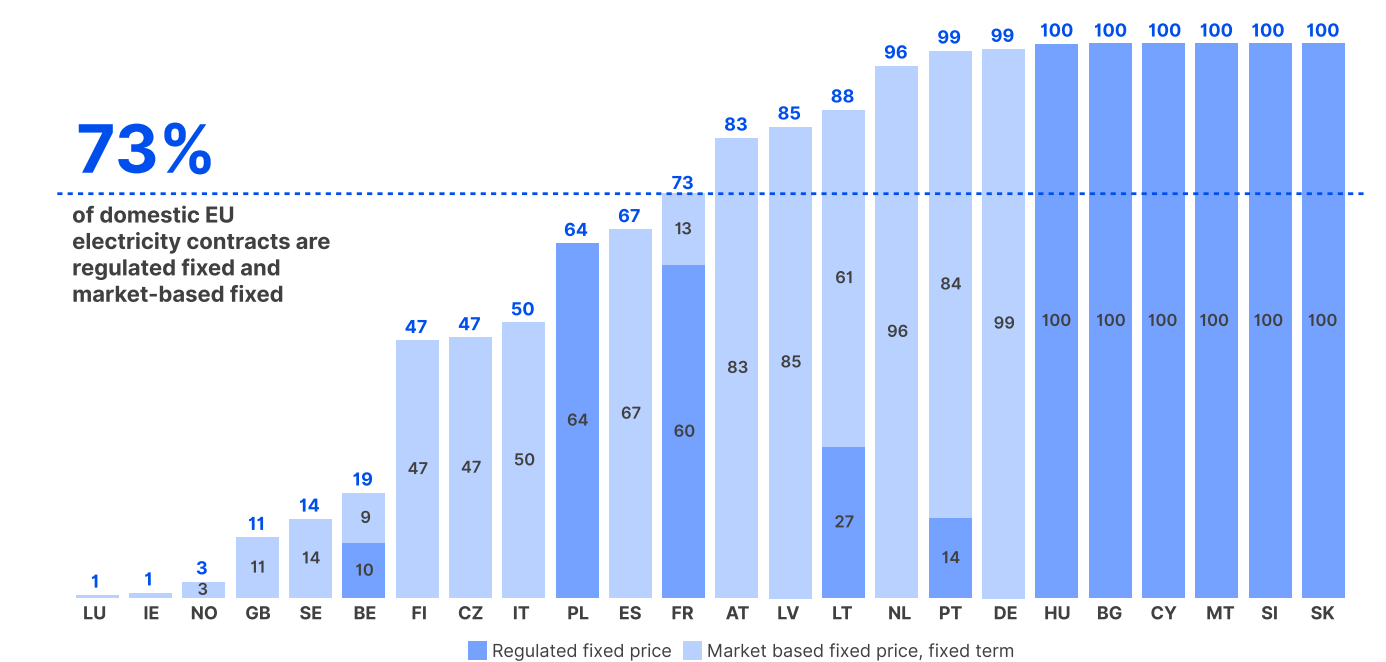
\includegraphics[width=1\linewidth]{figure/FP_EU.PNG}
%     \caption{Share of household fixed-contract contract uptake in Europe \cite{ACER2024} \hyperlink{options1}{\beamergotobutton{Options}}} 
%     \label{fig:FP_EU}
% \end{figure}

% \end{frame}

%%%%%%%%%%%%%%%%%%%%%%%%%%%%%%%%%%%%%%%%%%%%%%%%%%%%%%%%%%%%%%%%%%%%%%%%%%%%%%%%%%%%%%%%%%%%%%%%%%%%%%%%%%%%%%%%%%%%%%%%%%%%%%%%%%%%%%%%%%%%%%%%%%%%%%

\begin{frame}{Private contracts coexist with regulated options }\label{UptakeContract2}

\begin{figure}
    \centering
    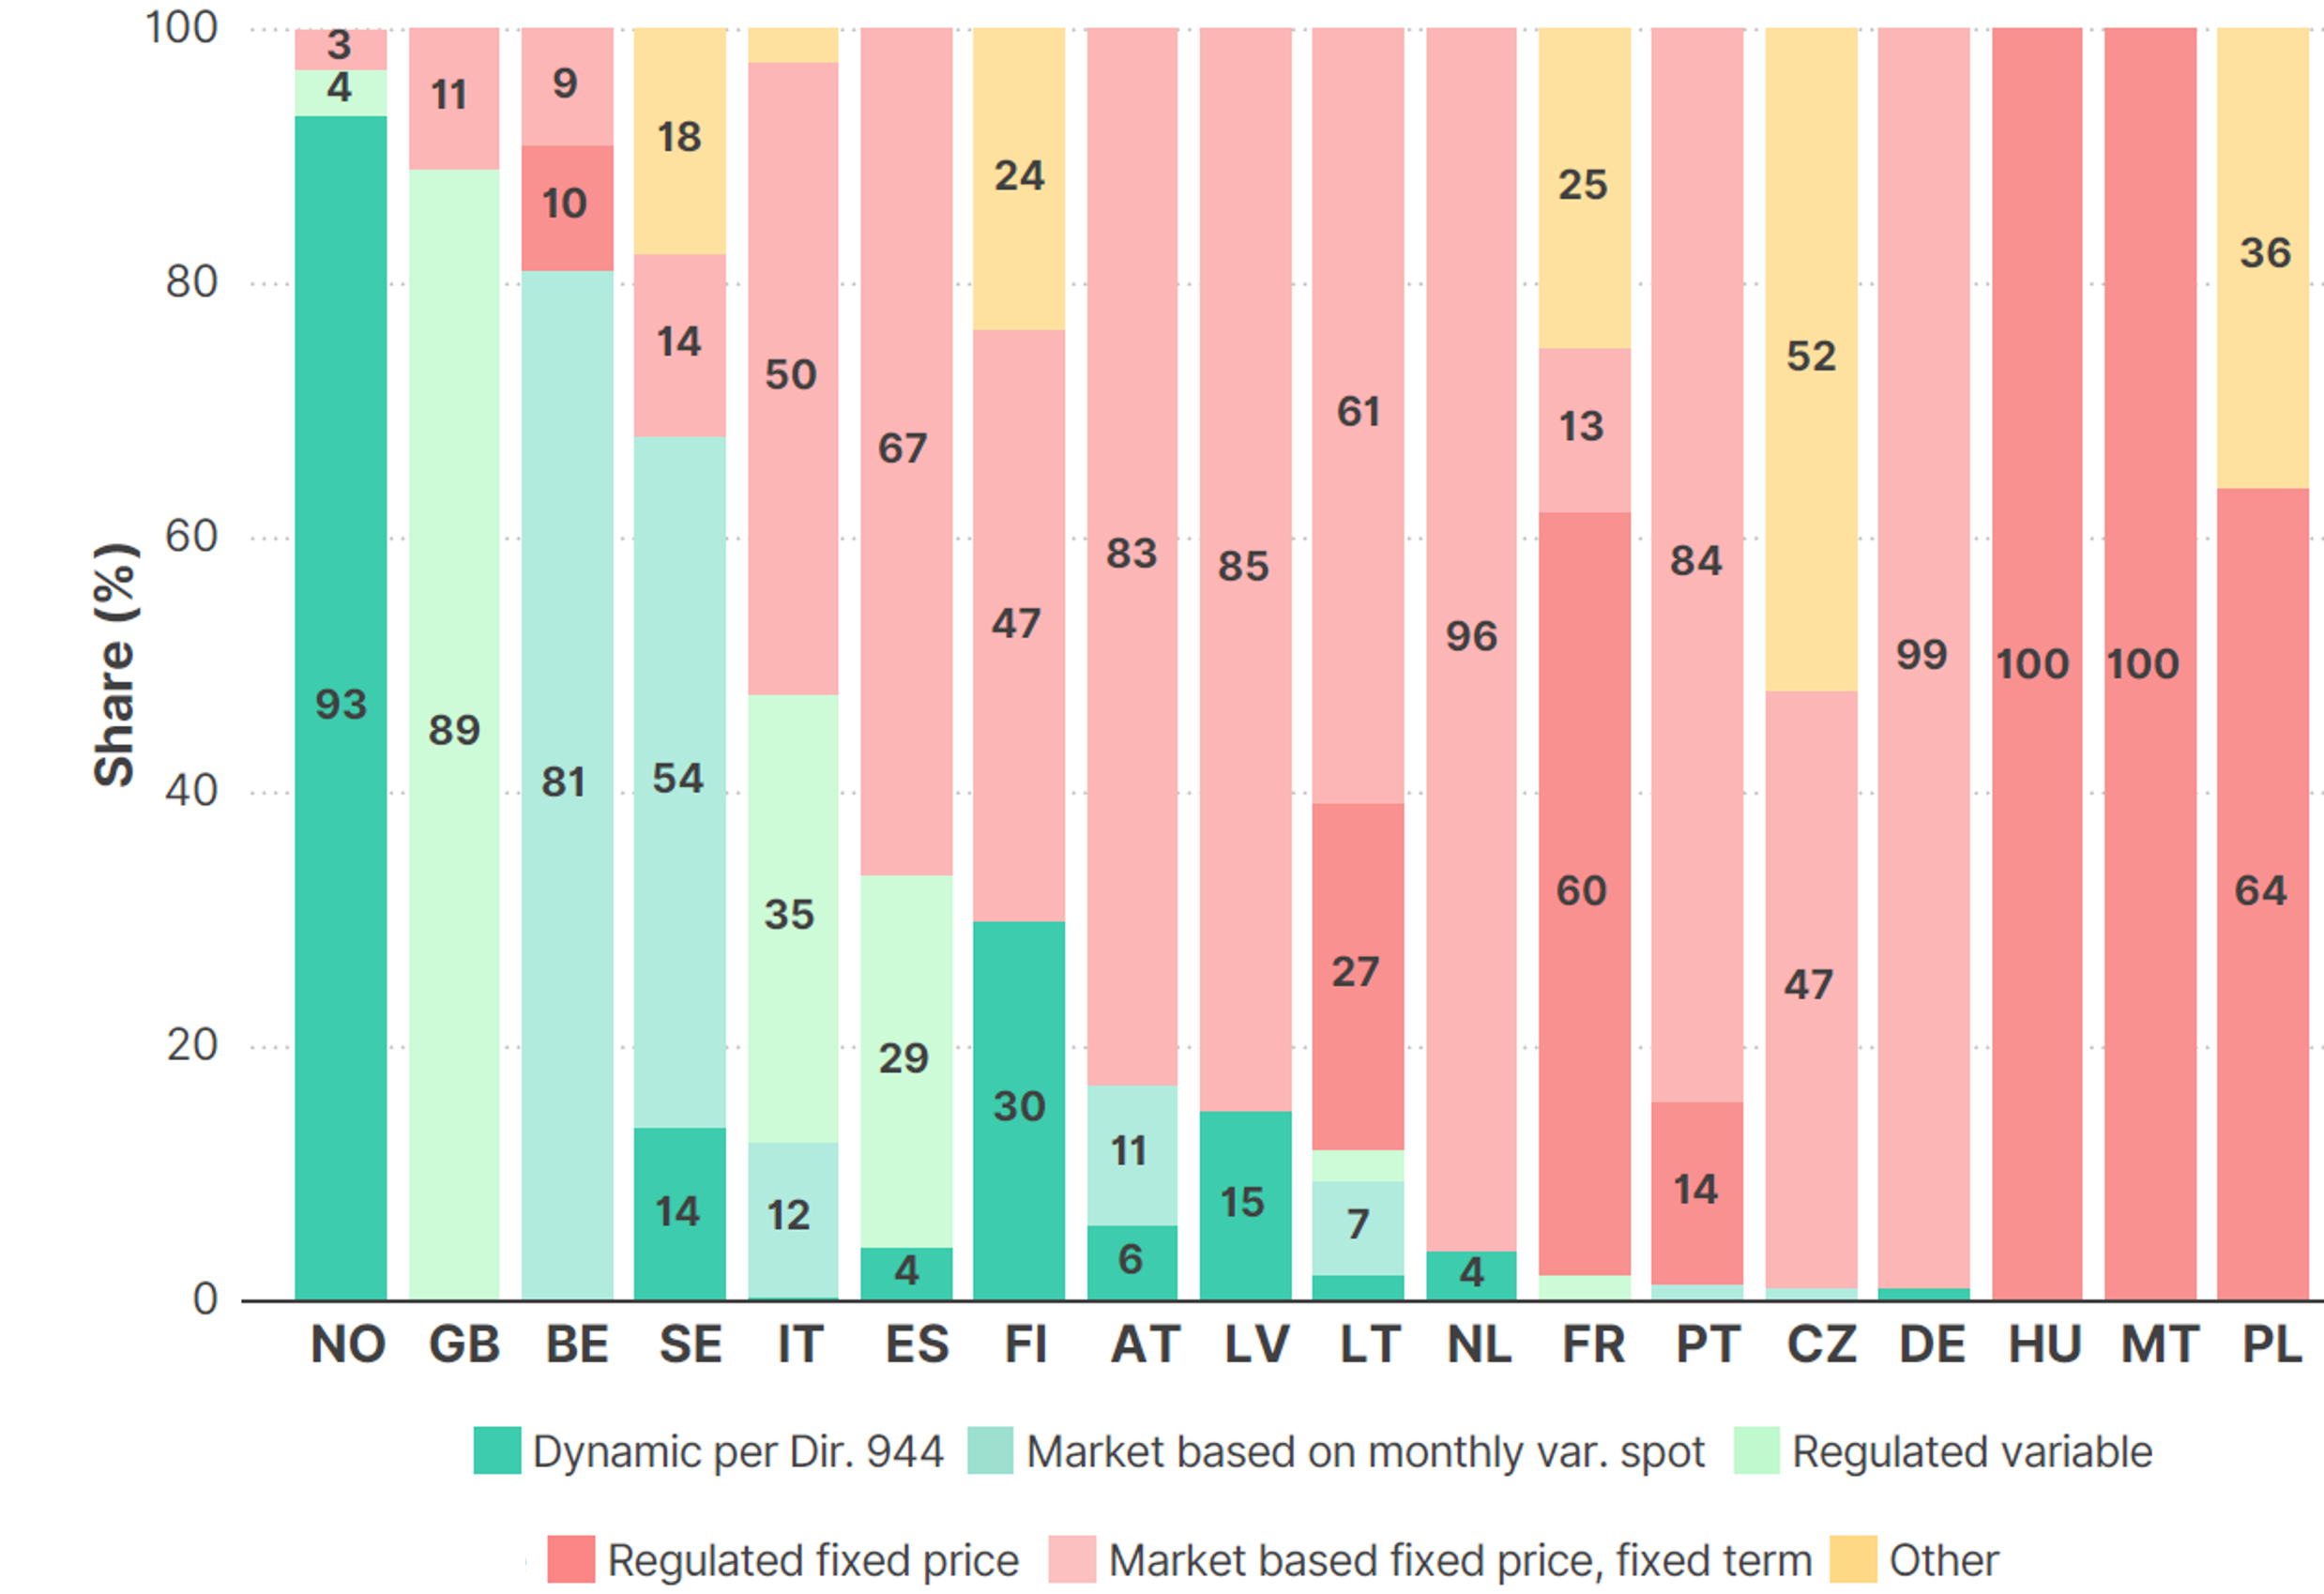
\includegraphics[width=0.8\linewidth]{figure/FP_EU_detail_v2.PNG}
    \caption{Share of household contract uptake in Europe \cite{ACER2024}} 
    \label{fig:FP_EU_detail}
\end{figure}

\end{frame}




%%%%%%%%%%%%%%%%%%%%%%%%%%%%%%%%%%%%%%%%%%%%%%%%%%%%%%%%%%%%%%%%%%%%%%%%%%%%%%%%%%%%%%%%%%%%%%%%%%%%%%%%%%%%%%%%%%%%%%%%%%%%%%%%%%%%%%%%%%%%%%%%%%%%%%



\begin{frame}{The set up}


\begin{itemize}

\item Provide a \boldrblue{stylized theoretical framework} where \vfill
\begin{itemize}
    \item A set of firms offers a fixed menu of contracts: 
    \begin{itemize}
        \item \boldrblue{a fixed-price (FP) and a dynamic-price (RTP) contract}
    \end{itemize} \vfill
    \item Consumer chooses a contract
    \begin{itemize}
        \item \boldrblue{commitment on price profile}
    \end{itemize} \vfill
    \item Consumers consume over \boldrblue{two periods}, and in each period different \boldrblue{willingness-to-pay} and \boldrblue{marginal production cost}.
    \end{itemize}
\end{itemize}

\vfill
\begin{itemize}
    \item \boldrblue{A selection market}: identity matters as cost depends on consumer types and contract choices.
\end{itemize}


\end{frame}

%%%%%%%%%%%%%%%%%%%%%%%%%%%%%%%%%%%%%%%%%%%%%%%%%%%%%%%%%%%%%%%%%%%%%%%%%%%%%%%%%%%%%%%%%%%%%%%%%%%%%%%%%%%%%%%%%%%%%%%%%%%%%%%%%%%%%%%%%%%%%%%%%%%%%%

\begin{frame}
\frametitle{Market Structure}
 
\vspace{-2pt}
 
\begin{center}
\scalebox{0.82}{%
\begin{tikzpicture}[node distance=0.45cm]

 \node[draw=notegray!30, fill=white, rounded corners=4pt,
      font=\small\itshape, text=notegray!80,
      inner sep=5pt, minimum width=13cm]
  (banner) at (0,0)
  {Retail Electricity Market};
  
% LEFT: PUBLIC FIRM
\node[firmbox=pubBlue, minimum width=5cm, minimum height=0.95cm,
      below left=0.55cm and 0.3cm of banner.south]
  (pubFirm)
  {\textcolor{pubBlue!15!black}{\textbf{\normalsize Public Firm}}\\[1pt]
   \textcolor{notegray}{\scriptsize regulated monopoly}};
 
\node[contractbox=fixOrange, minimum width=4.2cm,
      below=0.45cm of pubFirm]
  (pubFPC)
  {Fixed-Price Contract};
 
\node[below=0.35cm of pubFPC] (finTitle)
  {\textsc{Financing Mechanisms}};
 
\node[financebox, minimum width=4.2cm, below=0.12cm of finTitle]
  (fin1) {\textbf{(i)} \enspace \boldrblue{Shadow cost of public funds}};
 
\node[financebox, minimum width=4.2cm, below=0.1cm of fin1]
  (fin2) {\textbf{(ii)} \enspace Self-financing };
 
\node[financebox, minimum width=4.2cm, below=0.1cm of fin2]
  (fin3) {\textbf{(iii)} \enspace Market-wide tax};
 
 
 
% RIGHT: PRIVATE FIRMS
\node[firmbox=privGreen, minimum width=5cm, minimum height=0.95cm,
      below right=0.55cm and 0.3cm of banner.south]
  (privFirm)
  {\textcolor{privGreen!15!black}{\textbf{\normalsize Private Firms}}\\[1pt]
   \textcolor{notegray}{\scriptsize competitive fringe}};
 
\node[contractbox=fixOrange, minimum width=2.1cm, minimum height=1.1cm,
      below left=0.45cm and -2.55cm of privFirm]
  (privFPC)
  {Fixed-Price\\Contract};
 
\node[contractbox=dynPurple, minimum width=2.1cm, minimum height=1.1cm,
      below right=0.45cm and -2.55cm of privFirm]
  (privDPC)
  {Dynamic-Price\\Contract };

\end{tikzpicture}%
}
\end{center}

\vfill

\small
\begin{itemize}
    \item The public firm as a Universal Service Obligation, see Directive (EU) 2019/944
\end{itemize}

\end{frame}




%%%%%%%%%%%%%%%%%%%%%%%%%%%%%%%%%%%%%%%%%%%%%%%%%%%%%%%%%%%%%%%%%%%%%%%%%%%%%%%%%%%%%%%%%%%%%%%%%%%%%%%%%%%%%%%%%%%%%%%%%%%%%%%%%%%%%%%%%%%%%%%%%%%%%%

\begin{frame}{Main takeaways}


\begin{itemize}

\item \boldrblue{Optimal demand for contracts} \vfill

\begin{itemize}
    \item Higher willingness to pay during low-price periods $\rightarrow$ dynamic contract. Opposite for the FP contract.
\end{itemize}

\vfill

\item \boldrblue{Market equilibrium}.

\vfill

\begin{itemize}
    \item \boldrblue{Impossibility result}: FP contracts is not sustained at the equilibrium.     \vfill
    \begin{itemize}
    \item The option of a dynamic price contract unravels the FP market.  \vfill
    \item Hold for private firms and a self-financing public firm.
    \end{itemize}
    \vfill

\item \boldrblue{Advantageous selection} can be realized with public funds/taxes: \vfill

    \begin{center}
    W(\textcolor{blue}{Dynamic Private} +  \textcolor{red}{Fixed-Price Public})  { \textbf{  < }} W( \textcolor{red}{Fixed-Price Public})
   \end{center}

\vfill

\item Leakage of consumers to the private firms $\rightarrow$ low equilibrium fixed-price.

    \end{itemize}

\end{itemize}

\end{frame}


%%%%%%%%%%%%%%%%%%%%%%%%%%%%%%%%%%%%%%%%%%%%%%%%%%%%%%%%%%%%%%%%%%%%%%%%%%%%%%%%%%%%%%%%%%%%%%%%%%%%%%%%%%%%%%%%%%%%%%%%%%%%%%%%%%%%%%%%%%%%%%%%%%%%%%

\begin{frame}{Contributions}

\begin{itemize}

\item  Consumers differ in \boldrblue{willingness-to-pay} across consumption period.

\vfill

\begin{itemize}
    \item Extend exogenous share papers. \cite{Borenstein2005b,Leautier2014,Ambec2021,Boom2021}
 
 \vfill
 
 \item Extend single type consumers model. \cite{joskow2006retail,Astier2021,ancel2025tariffs}
    \end{itemize}

\vfill

\item We model \boldrblue{retail competition} between firms that offer the two contracts. 

\vfill

\begin{itemize}
    \item Scarce literature \cite{joskow2006retail}, \cite{Borenstein2003} and \cite{ancel2025tariffs}

\vfill

        \item Adverse Selection \cite{1970Akerlof}, price theory \cite{Einav2012,Veiga2023}, product design \cite{Veiga2016}, competition \cite{Azevedo2017}
\vfill

\item Regulation theory \cite{laffont1993theory}, public vs private options \cite{Martimort2020a,Kang2023a}.

\end{itemize}
\end{itemize}

\end{frame}

%%%%%%%%%%%%%%%%%%%%%%%%%%%%%%%%%%%%%%%%%%%%%%%%%%%%%%%%%%%%%%%%%%%%%%%%%%%%%%%%%%%%%%%%%%%%%%%%%%%%%%%%%%%%%%%%%%%%%%%%%%%%%%%%%%%%%%%%%%%%%%%%%%%%%%
%%%%%%%%%%%%%%%%%%%%%%%%%%%%%%%%%%%%%%%%%%%%%%%%%%%%%%%%%%%%%%%%%%%%%%%%%%%%%%%%%%%%%%%%%%%%%%%%%%%%%%%%%%%%%%%%%%%%%%%%%%%%%%%%%%%%%%%%%%%%%%%%%%%%%%
%%%%%%%%%%%%%%%%%%%%%%%%%%%%%%%%%%%%%%%%%%%%%%%%%%%%%%%%%%%%%%%%%%%%%%%%%%%%%%%%%%%%%%%%%%%%%%%%%%%%%%%%%%%%%%%%%%%%%%%%%%%%%%%%%%%%%%%%%%%%%%%%%%%%%%

\section{The model}

\begin{frame}{Roadmap}
  \tableofcontents [sectionstyle=show/shaded,subsectionstyle=show/shaded]
\end{frame}



%%%%%%%%%%%%%%%%%%%%%%%%%%%%%%%%%%%%%%%%%%%%%%%%%%%%%%%%%%%%%%%%%%%%%%%%%%%%%%%%%%%%%%%%%%%%%%%%%%%%%%%%%%%%%%%%%%%%%%%%%%%%%%%%%%%%%%%%%%%%%%%%%%%%%%

\begin{frame}{Consumers}

\begin{itemize}
    \item A unit mass of consumers.

\vfill

    \item With a \boldrblue{unit demand} for electricity for each two periods $t = 1,2$.

\vfill

    \item A \boldrblue{two-dimensional} type $\textbf{v}=(v_1,v_2) $
    
\vfill

        % \begin{itemize}
 \item Drawn from a pdf. $f(v)$ and cdf. $F(v)$ with support $[\underline{v}_t,\bar{v}_t]$. 
            
% \vfill

        % \item Even though the distributions are independent, we assume the affine relationship between the two periods, where $\alpha,\beta \in \mathbb{R}$.

% \end{itemize}

        % \begin{equation*}
        %     [ \ubar{v}_2, \bar{v}_2] = [\alpha + \beta \ubar{v}_1, \alpha + \beta \bar{v}_1]
        % \end{equation*}


\vfill

\item Type $\textbf{v}$ consumer surplus from consuming at price profile $\textbf{p}$ is:

\begin{equation*}
 u\left(\textbf{v},\textbf{p}\right)= v_1-p_1 +  v_2-p_2
 \end{equation*}
\end{itemize}    
\end{frame}


%%%%%%%%%%%%%%%%%%%%%%%%%%%%%%%%%%%%%%%%%%%%%%%%%%%%%%%%%%%%%%%%%%%%%%%%%%%%%%%%%%%%%%%%%%%%%%%%%%%%%%%%%%%%%%%%%%%%%%%%%%%%%%%%%%%%%%%%%%%%%%%%%%%%%%

\begin{frame}{Retailers}

\begin{itemize}
    \item We assume a set of retailers that purchase at no additional cost on the wholesale market at \boldrblue{price} $c_t$. \vfill
    \begin{itemize}
        \item We assume w.l.o.g. that $c_1 < c_2$ 
    \end{itemize}
    

    \vfill

    \item We take the characteristics of contracts and the set of contracts as given.  \vfill
    
    \item If $\textbf{p}^k=(p_1^k,p_2^k)$ is profile unit-price of contract $k$ then:  \vfill

    \begin{itemize}
        \item FP contract: $\textbf{p}^{r} =  (p^r,p^r)$  \vfill
        \item Dynamic contract: $\textbf{p}^{s} =  (p_1,p_2)$
    \end{itemize}

\vfill

\item Fixed part of a Two-Part tariff: $A^k$.

\end{itemize}


    
\end{frame}

%%%%%%%%%%%%%%%%%%%%%%%%%%%%%%%%%%%%%%%%%%%%%%%%%%%%%%%%%%%%%%%%%%%%%%%%%%%%%%%%%%%%%%%%%%%%%%%%%%%%%%%%%%%%%%%%%%%%%%%%%%%%%%%%%%%%%%%%%%%%%%%%%%%%%%

\begin{frame}{Equilibrium Definition - Consumer}

\small
\begin{itemize}

\item The optimal consumer choose a consumption profile $\textbf{x} = (x_1,x_2)$ with $x_t \in\{0,1\}$, given a contract, to maximize its utility:

\vfill

\begin{equation*}
    U(\mathbf{v}, k) = \max_{\mathbf{x} \in \{0,1\}^2} \left\{ \mathbf{x} \cdot (\mathbf{v} - \mathbf{p}^k) - A^k \mathbb{I}_{\{\mathbf{x} \neq \mathbf{0}\}} \right\}
\end{equation*}

\vfill

\item The \textit{participation set} for contract $k$ given an optimal profile $\textbf{x}^\ast$ is:

\begin{equation*} \label{eq:active_set_general}
    \mathcal{S}^k = \left\{ \mathbf{v} \in V : \mathbf{x}^*(\mathbf{v},k) \neq \mathbf{0} \quad \text{and} \quad k \in \arg\max_{j \in \{r,s\}} U(\mathbf{v}, j) \right\}.
\end{equation*}

\vfill

\item $\mu^k$ denotes the mass of consumers $k$ and $q_t^k$ the demand in period $t$ is:
  \vfill

\begin{equation*}
    \mu^k = \int_{\mathcal{S}^k} f(\mathbf{v}) \, d\mathbf{v} \qquad \qquad  q_t^k = \int_{\mathcal{S}^k} x_t^*(\mathbf{v}, k) f(\mathbf{v}) \, d\mathbf{v}.
\end{equation*}

 where  $\mathbf{q}^k:= (q^k_1,q^k_2)$. Consumer surplus:


 \begin{equation*}
    CS^k
    =
    \int_{\mathcal{S}^k}
    \left[
    \sum_{t\in\{1,2\}}
    x_t^*(\mathbf{v},k)
    \left(v_t-p_t^k\right)
    -
    A^k
    \right]
    f(\mathbf{v})\,d\mathbf{v}.
\end{equation*}

\end{itemize}
    
\end{frame}


%%%%%%%%%%%%%%%%%%%%%%%%%%%%%%%%%%%%%%%%%%%%%%%%%%%%%%%%%%%%%%%%%%%%%%%%%%%%%%%%%%%%%%%%%%%%%%%%%%%%%%%%%%%%%%%%%%%%%%%%%%%%%%%%%%%%%%%%%%%%%%%%%%%%%%



\begin{frame}{Equilibrium Definition - Firms}


\begin{itemize}

\item The equilibrium prices $(\mathbf{p}^k,A^k)$ are pinned down by the zero-profit condition:
\vfill
    \begin{equation*}
        \pi^k  = \mathbf{q}^k \cdot \mathbf{p}^k  +  \mu^k A^k -  TC^k = 0
    \end{equation*}

 where 

\begin{equation*}
    TC^k
    =
    \sum_{t\in\{1,2\}}
    \int_{\mathcal{S}^k}
    c_t x_t^*(\mathbf{v}, k) f(\mathbf{v}) \, d\mathbf{v}.
\end{equation*}

\vfill
\item We restrict the \textit{public firm} to offer the FP contract, and the equilibrium tariff
$(p^r,A^r)$ maximizes its objective:

\vfill
\[
    (p^r,A^r)\in 
    \arg\max_{p^r,A^r}
    \left\{
    \Omega^r(p^r,A^r)
    =
    CS^r(p^r,A^r)
    + (1+\lambda) \pi^r(p^r,A^r)
    \right\}.
\]

\vfill

\item $\lambda>0$ is the marginal cost of public funds.

\end{itemize}

\end{frame}
%%%%%%%%%%%%%%%%%%%%%%%%%%%%%%%%%%%%%%%%%%%%%%%%%%%%%%%%%%%%%%%%%%%%%%%%%%%%%%%%%%%%%%%%%%%%%%%%%%%%%%%%%%%%%%%%%%%%%%%%%%%%%%%%%%%%%%%%%%%%%%%%%%%%%%


% \begin{frame}{Example with one contract}
% \begin{figure}
%     \centering
%     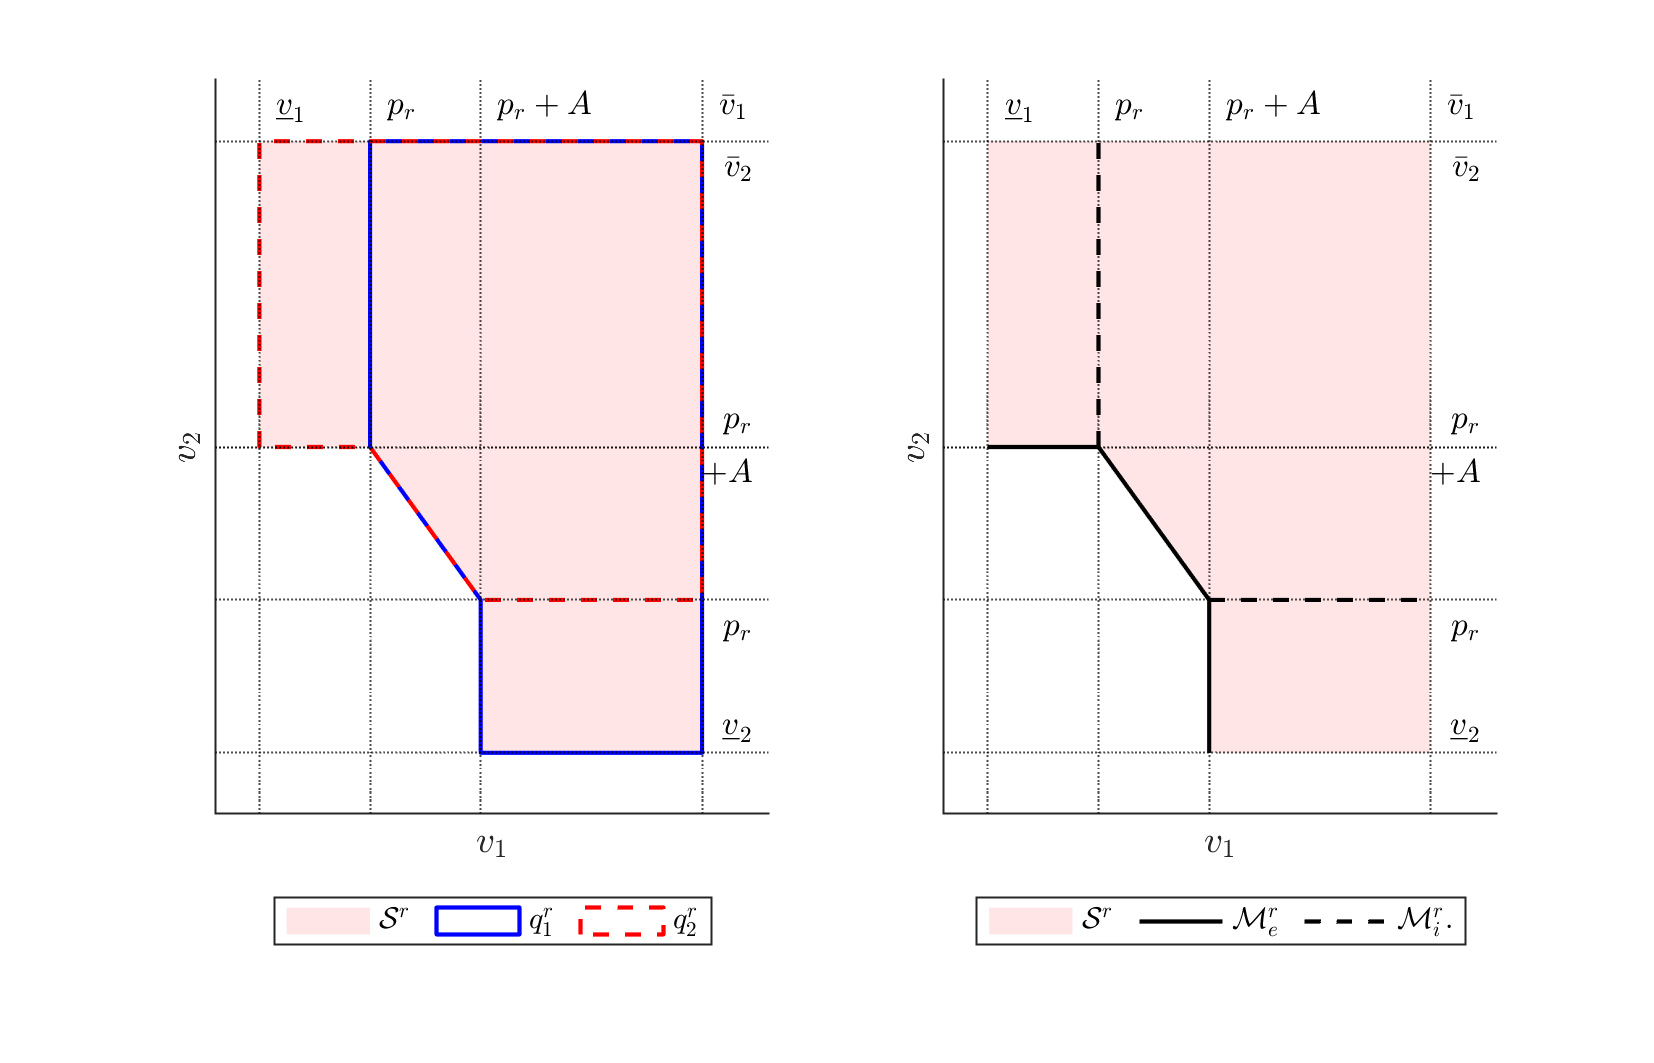
\includegraphics[width=1\linewidth]{figure/intro_zone_A_ppt.png}
%     \caption{Demand for the fixed-price contract, and marginal consumers (\textit{exiters and profile switchers}).}
%     \label{fig:intro_zone_mu}
% \end{figure}


% \end{frame}
% %%%%%%%%%%%%%%%%%%%%%%%%%%%%%%%%%%%%%%%%%%%%%%%%%%%%%%%%%%%%%%%%%%%%%%%%%%%%%%%%%%%%%%%%%%%%%%%%%%%%%%%%%%%%%%%%%%%%%%%%%%%%%%%%%%%%%%%%%%%%%%%%%%%%%%

% \begin{frame}{Single Contract Equilibrium}

% \begin{itemize}

%  \item If private retailers offer the FP contract, then the linear price is the eq. and takes the following form:

% \begin{equation*}
%  p^r^{av} =  \text{av. total cost}   \quad \text{and} \quad A_r^* =0 
% \end{equation*}

% \vfill

% \item If private retailers offer the RTP contract, then competition implies full cost pass-through to consumers:

% \vfill

% \begin{equation*}
%  \textbf{p}_s^*  = \{p_1^w,p_2^w\}  = \{c_1,c_2\}   \quad \text{and} \quad A_s^* =0 
% \end{equation*}

% \vfill

% \item If the public firm offers the FP contract, then: 

% \vfill

%         \begin{equation*}
%             p^r^{**} \quad = \quad \text{av.marg.cost} \quad + \quad \text{ramsey A}  \quad- \quad \underbrace{\bigg.A^{**}_r \frac{\delta_A\mu_r}{\delta_A q^r} \bigg.}_{\text{switchers wedge}}
%         \end{equation*}



% \end{itemize}

% \end{frame}

%%%%%%%%%%%%%%%%%%%%%%%%%%%%%%%%%%%%%%%%%%%%%%%%%%%%%%%%%%%%%%%%%%%%%%%%%%%%%%%%%%%%%%%%%%%%%%%%%%%%%%%%%%%%%%%%%%%%%%%%%%%%%%%%%%%%%%%%%%%%%%%%%%%%%%

% \begin{frame}{Adverse Selection in Single Contract Equilibrium}

% \begin{itemize}

% \item We derive sufficient and necessary conditions for the private and public equilibrium to exhibit adverse (or advantageous) selection.  \vfill

% \item  Private equilibrium (sufficient conditions):   \vfill

% \begin{equation*}
%  \frac{\# \text{marginal cons. in 1}}{\# \text{ cons. in 1}} > \frac{\# \text{marginal cons. in 2}}{\# \text{ cons. in 2}}   
% \end{equation*}

% \vfill

% \item  Public equilibrium (necessary conditions):   \vfill

% \begin{equation*}
%  \frac{\# \text{profile switchers in 1}}{\# \text{ cons. in 1}} <  (>)  \frac{\# \text{profile switchers in 2}}{\# \text{cons. in 2}}   \quad \text{and} \quad \lambda > (<)1 
% \end{equation*}

% \end{itemize}

% \end{frame}


%%%%%%%%%%%%%%%%%%%%%%%%%%%%%%%%%%%%%%%%%%%%%%%%%%%%%%%%%%%%%%%%%%%%%%%%%%%%%%%%%%%%%%%%%%%%%%%%%%%%%%%%%%%%%%%%%%%%%%%%%%%%%%%%%%%%%%%%%%%%%%%%%%%%%%

\begin{frame}{Timing of contract choice}
\centering
\resizebox{\textwidth}{!}{%
\begin{tikzpicture}[
    >=Latex,
    thick,
    every node/.style={font=\scriptsize},
    dot/.style={circle,fill=black,inner sep=1.8pt},
    choice/.style={circle,draw,minimum size=7mm,inner sep=0pt},
    lab/.style={align=center,font=\scriptsize},
    brace/.style={decorate,decoration={brace,amplitude=5pt}}
]

% Nodes
\node[dot] (start) at (0,0) {};
\node[choice] (draw) at (2.0,0) {$C$};

\node[choice] (fp) at (3.1,1.2) {$RTP$};
\node[choice] (rtp) at (3.1,-1.2) {$FP$};

\node[choice] (fp1) at (5.0,1.2) {$C$};
\node[choice] (rtp1) at (5.0,-1.2) {$C$};

\node[choice] (fp2) at (8.3,1.2) {$C$};
\node[choice] (rtp2) at (8.3,-1.2) {$C$};

\node[dot] (endfp) at (11.4,1.2) {};
\node[dot] (endrtp) at (11.4,-1.2) {};

% Outside option
\node[dot] (outside) at (2.0,-2.35) {};

% Arrows
\draw[->] (start) -- node[above] {$v_1,v_2$ drawn} (draw);

\draw[->] (draw) -- (fp);
\draw[->] (draw) -- (rtp);

\draw[->] (draw.south) -- node[left] {No contract} (outside);
\node[lab, below=0.08cm of outside] {$0$};

\draw[->] (fp) -- node[above] {Pay $A^s$} (fp1);
\draw[->] (rtp) -- node[above] {Pay $A^r$} (rtp1);

\draw[->] (fp1) -- node[above] {Buy at $p_1$} (fp2);
\draw[->] (rtp1) -- node[above] {Buy at $p^r$} (rtp2);

\draw[->] (fp2) -- node[above] {Buy at $p_2$} (endfp);
\draw[->] (rtp2) -- node[above] {Buy at $p^r$} (endrtp);

% FP payoff labels
\node[lab] at (6.45,0.35)
{$u_1^{r}=[v_1-p_1]^+$\\[5pt]
$\Pi_1^{r}=(p_1-c_1)\mathbf{1}\{v_1\geq p_1\}$};

\node[lab] at (9.75,0.35)
{$u_2^{r}=[v_2-p_2]^+$\\[5pt]
$\Pi_2^{r}=(p_2-c_2)\mathbf{1}\{v_2\geq p_2\}$};

% RTP payoff labels
\node[lab] at (6.45,-2.05)
{$u_1^{s}=[v_1-p^r]^+$\\[5pt]
$\Pi_1^{s}=(p^r-c_1)\mathbf{1}\{v_1\geq p^r\}$};

\node[lab] at (9.75,-2.05)
{$u_2^{s}=[v_2-p^r]^+$\\[5pt]
$\Pi_2^{s}=(p^r-c_2)\mathbf{1}\{v_2\geq p^r\}$};

% Final utilities
\node[lab, right=0.15cm of endfp]
{$U^{s}=u_1^{s}+u_2^{s}-A^s$};

\node[lab, right=0.15cm of endrtp]
{$U^{r}=u_1^{r}+u_2^{r}-A^r$};

% Braces
\draw[brace] (5,2.1) -- (8.3,2.1)
node[midway,yshift=0.45cm] {$t=1$};

\draw[brace] (8.3,2.1) -- (11.4,2.1)
node[midway,yshift=0.45cm] {$t=2$};

\end{tikzpicture}
}
\end{frame}

%%%%%%%%%%%%%%%%%%%%%%%%%%%%%%%%%%%%%%%%%%%%%%%%%%%%%%%%%%%%%%%%%%%%%%%%%%%%%%%%%%%%%%%%%%%%%%%%%%%%%%%%%%%%%%%%%%%%%%%%%%%%%%%%%%%%%%%%%%%%%%%%%%%%%%

% \subsection{Single contract benchmark equilibrium}

%%%%%%%%%%%%%%%%%%%%%%%%%%%%%%%%%%
%%%%%%%%%%%%%%%%%%%%%%%%%%%%%%%%%%%%%%%%%%%%%%%%%%%%%%%%%%%%%%%%%%%%%%%%%%%%%%%%%%%%%%%%%%%%%%%%%%%%%%%%%%%%%%%%%%%%%%%%%%%%%%%%%%%%%%%%%%%%%%%%%%%%%%


\begin{frame}{The single contract case}\label{single}

\begin{figure}
    \centering
    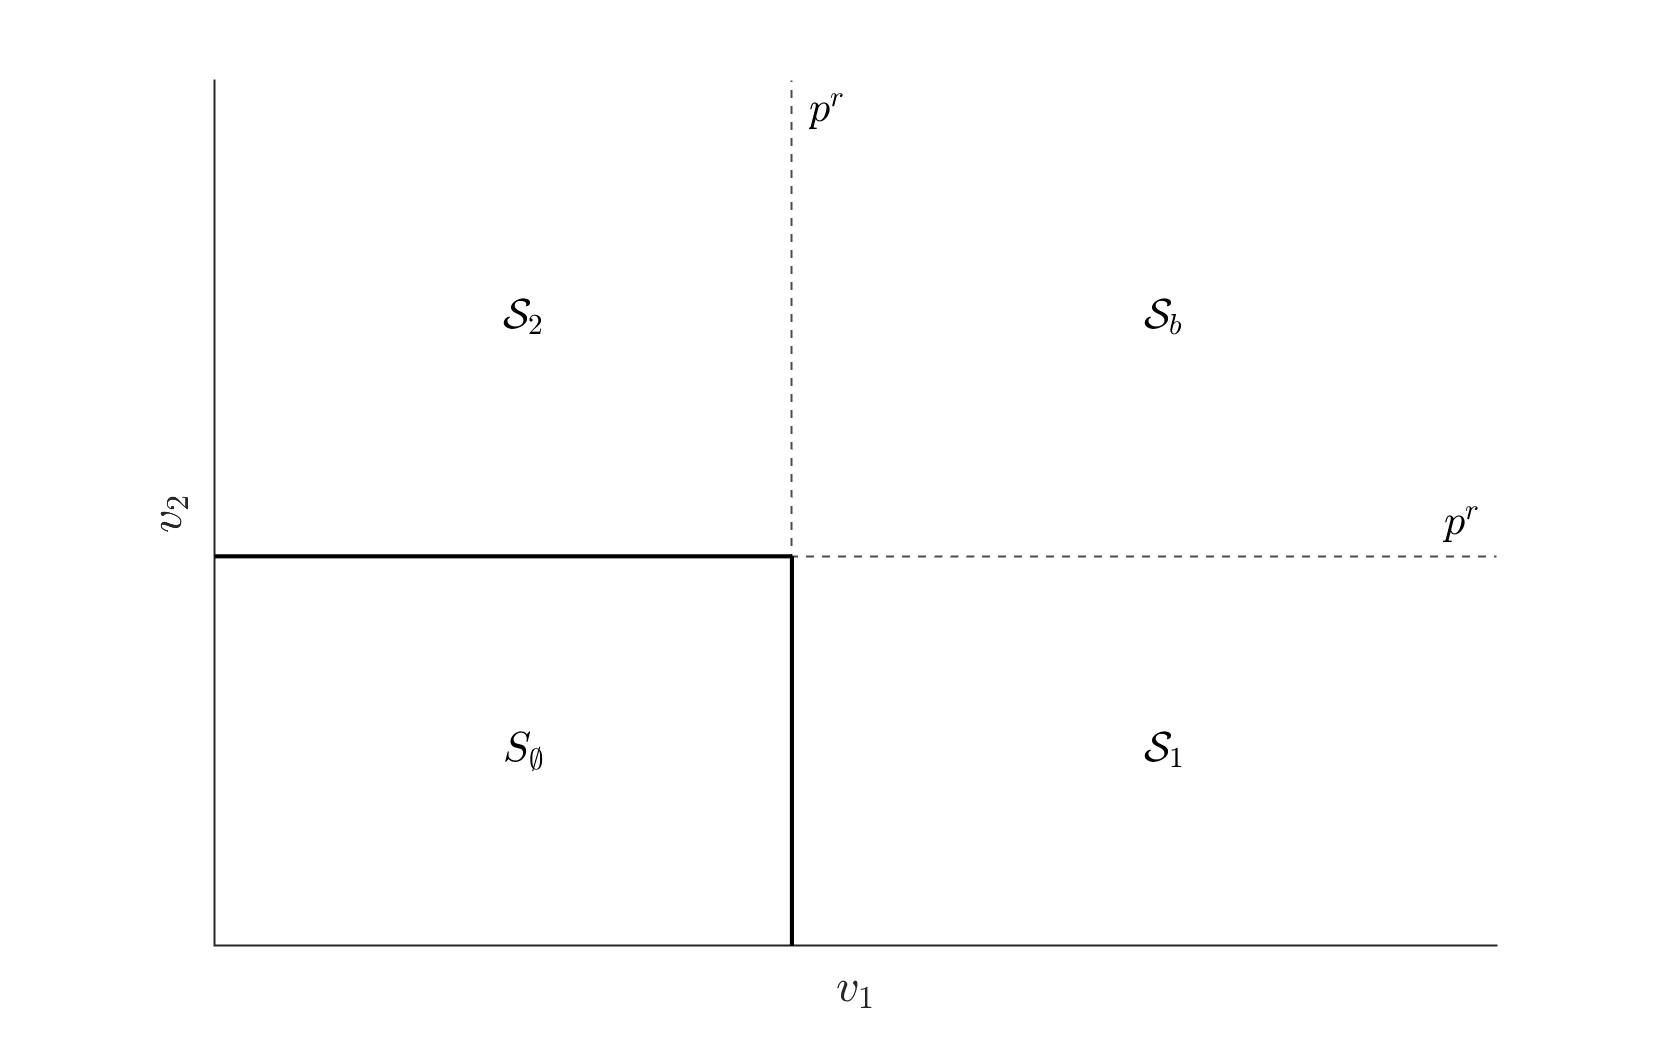
\includegraphics[width=0.8\linewidth]{figure/fp_demand_multi.png}
     \caption{The canonical bundle case. $S_t$ denotes the set of consumers consuming only in period $t$, and $S_b$ in the two period. \hyperlink{EquilibriumSingle}{\beamerreturnbutton{Equilibrium}}  \hyperlink{Adverse}{\beamerreturnbutton{Adverse Selection}} }     

    \label{fig:fp_demand_multi}
\end{figure}
    
\end{frame}

%%%%%%%%%%%%%%%%%%%%%%%%%%%%%%%%%%%%%%%%%%%%%%%%%%%%%%%%%%%%%%%%%%%%%%%%%%%%%%%%%%%%%%%%%%%%%%%%%%%%%%%%%%%%%%%%%%%%
%%%%%%%%%%%%%%%%%%%%%%%%%%%%%%%%%%%%%%%%%%%%%%%%%%%%%%%%%%%%%%%%%%%%%%%%%%%%%%%%%%%%%%%%%%%%%%%%%%%%%%%%%%%%%%%%%%%%%%%%%%%%%%%%%%%%%%%%%%%%%%%%%%%%%%
%%%%%%%%%%%%%%%%%%%%%%%%%%%%%%%%%%%%%%%%%%%%%%%%%%%%%%%%%%%%%%%%%%%%%%%%%%%%%%%%%%%%%%%%%%%%%%%%%%%%%%%%%%%%%%%%%%%%%%%%%%%%%%%%%%%%%%%%%%%%%%%%%%%%%%
%%%%%%%%%%%%%%%%%%%%%%%%%%%%%%%%%%%%%%%%%%%%%%%%%%%%%%%%%%%%%%%%%%%%%%%%%%%%%%%%%%%%%%%%%%%%%%%%%%%%%%%%%%%%%%%%%%%%%%%%%%%%%%%%%%%%%%%%%%%%%%%%%%%%%%

%%%%%%%%%%%%%%%%%%%%%%%%%%%%%%%%%%%%%%%%%%%%%%%%%%%%%%%%%%%%%%%%%%%%%%%%%%%%%%%%%%%%%%%%%%%%%%%%%%%%%%%%%%%%%%%%%%%%%%%%%%%%%%%%%%%%%%%%%%%%%%%%%%%%%%
%%%%%%%%%%%%%%%%%%%%%%%%%%%%%%%%%%%%%%%%%%%%%%%%%%%%%%%%%%%%%%%%%%%%%%%%%%%%%%%%%%%%%%%%%%%%%%%%%%%%%%%%%%%%%%%%%%%%%%%%%%%%%%%%%%%%%%%%%%%%%%%%%%%%%%
%%%%%%%%%%%%%%%%%%%%%%%%%%%%%%%%%%%%%%%%%%%%%%%%%%%%%%%%%%%%%%%%%%%%%%%%%%%%%%%%%%%%%%%%%%%%%%%%%%%%%%%%%%%%%%%%%%%%%%%%%%%%%%%%%%%%%%%%%%%%%%%%%%%%%%

\section{Partial equilibrium}


\begin{frame}{Roadmap}
  \tableofcontents [sectionstyle=show/shaded,subsectionstyle=show/shaded]
\end{frame}



%%%%%%%%%%%%%%%%%%%%%%%%%%%%%%%%%%%%%%%%%%%%%%%%%%%%%%%%%%%%%%%%%%%%%%%%%%%%%%%%%%%%%%%%%%%%%%%%%%%%%%%%%%%%%%%%%%%%%%%%%%%%%%%%%%%%%%%%%%%%%%%%%%%%%%


\begin{frame}{The marginal consumers}


\begin{itemize}

\item Contract prices as given:   
\begin{itemize}
    \item $A^k =0 $
    \item  $p_1 < p^r < p_2$
    \item $\bar{p} = \mathbb{E}[p_t]$ \vfill
\end{itemize}


\item Marginal consumers $\equiv $ same utility over at least two options when optimizing over the set of contracts and consumption profiles.

\vfill

\item There are three types

\vfill

\begin{itemize}
    \item \textit{Exiters} - stop consuming  ($   \mathcal{M}^k_e$) \vfill
    \item \textit{Profile switchers} - 2 periods vs 1 period in the same contract  ($\mathcal{M}^k_i$) \vfill
    \item \boldrblue{Contract switchers} - switch contract and consumption profile  ($   \mathcal{M}^\Delta_{a,b}$)
\end{itemize}



\end{itemize}

\end{frame}
%%%%%%%%%%%%%%%%%%%%%%%%%%%%%%%%%%%%%%%%%%%%%%%%%%%%%%%%%%%%%%%%%%%%%%%%%%%%%%%%%%%%%%%%%%%%%%%%%%%%%%%%%%%%%%%%%%%%%%%%%%%%%%%%%%%%%%%%%%%%%%%%%%%%%%

\begin{frame}{The marginal consumers}\label{PlotIndifConso}

\begin{figure}
    \centering
    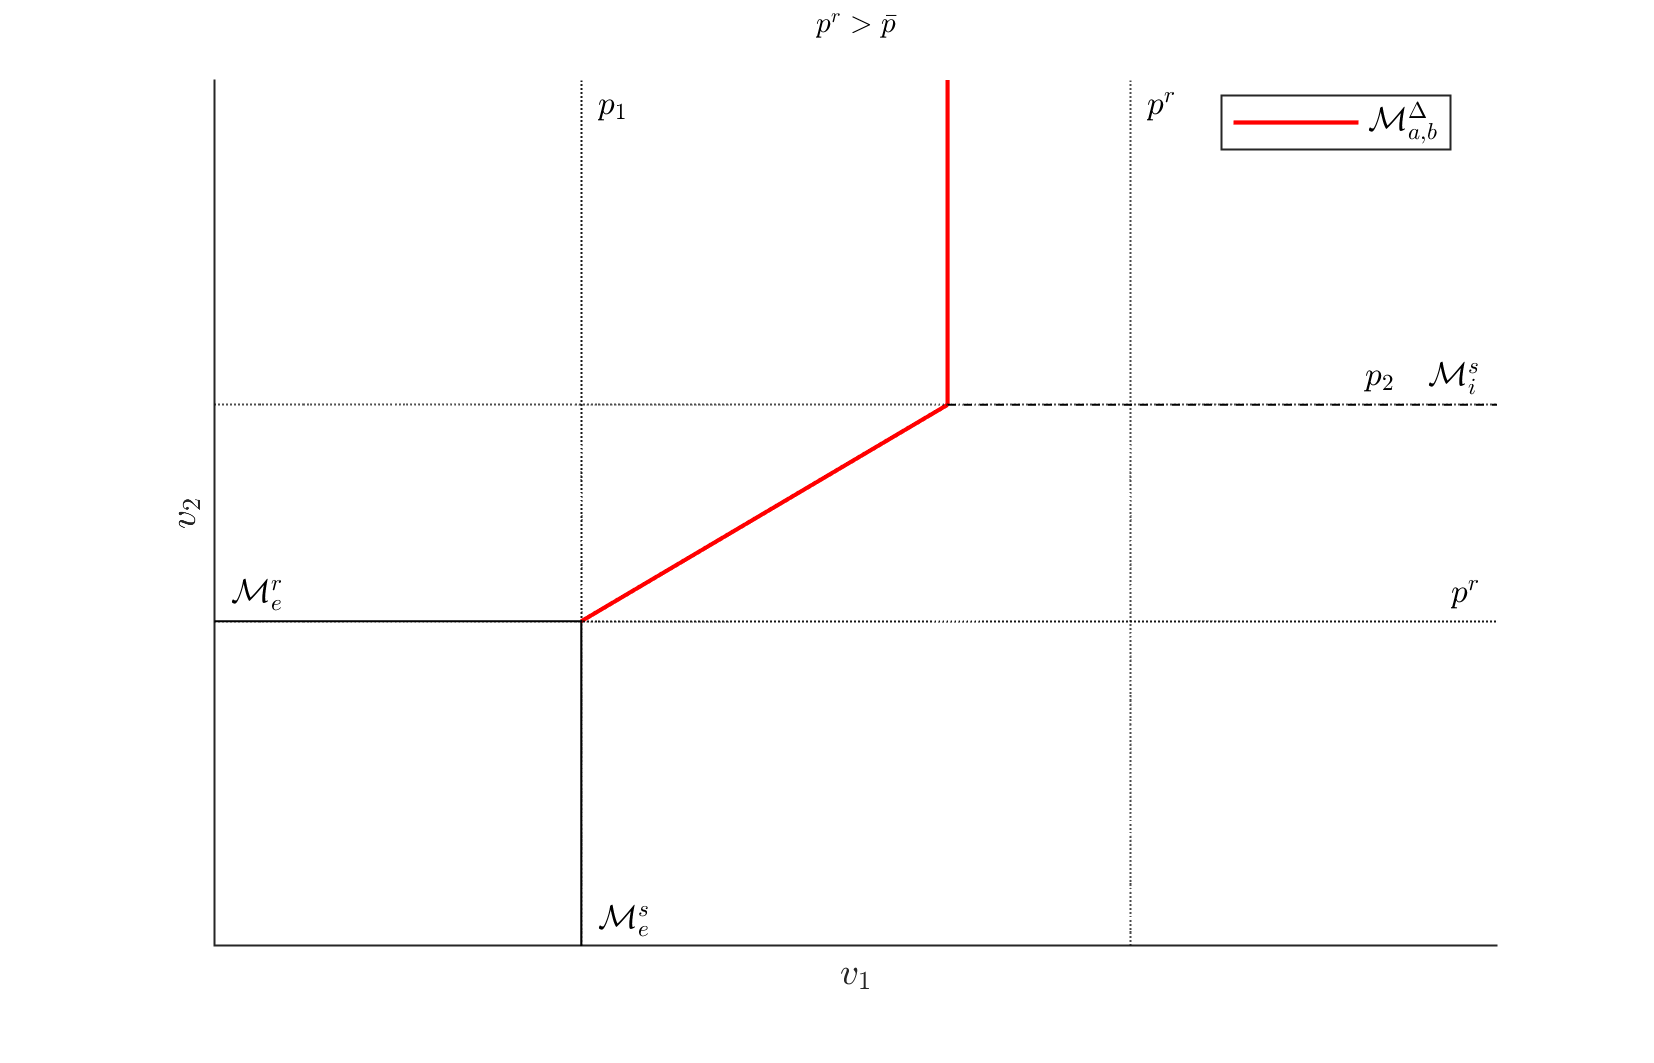
\includegraphics[width=1\linewidth]{figure/example_cstc_ppt1.png}
     \caption{Contract switchers are defined by the red lines.} 
    \label{fig:example_cstc_ppt1}
\end{figure}
    
\end{frame}

%%%%%%%%%%%%%%%%%%%%%%%%%%%%%%%%%%%%%%%%%%%%%%%%%%%%%%%%%%%%%%%%%%%%%%%%%%%%%%%%%%%%%%%%%%%%%%%%%%%%%%%%%%%%%%%%%%%%%%%%%%%%%%%%%%%%%%%%%%%%%%%%%%%%%%

\begin{frame}{The demand for contracts}\label{demand1}

\begin{figure}
    \centering
    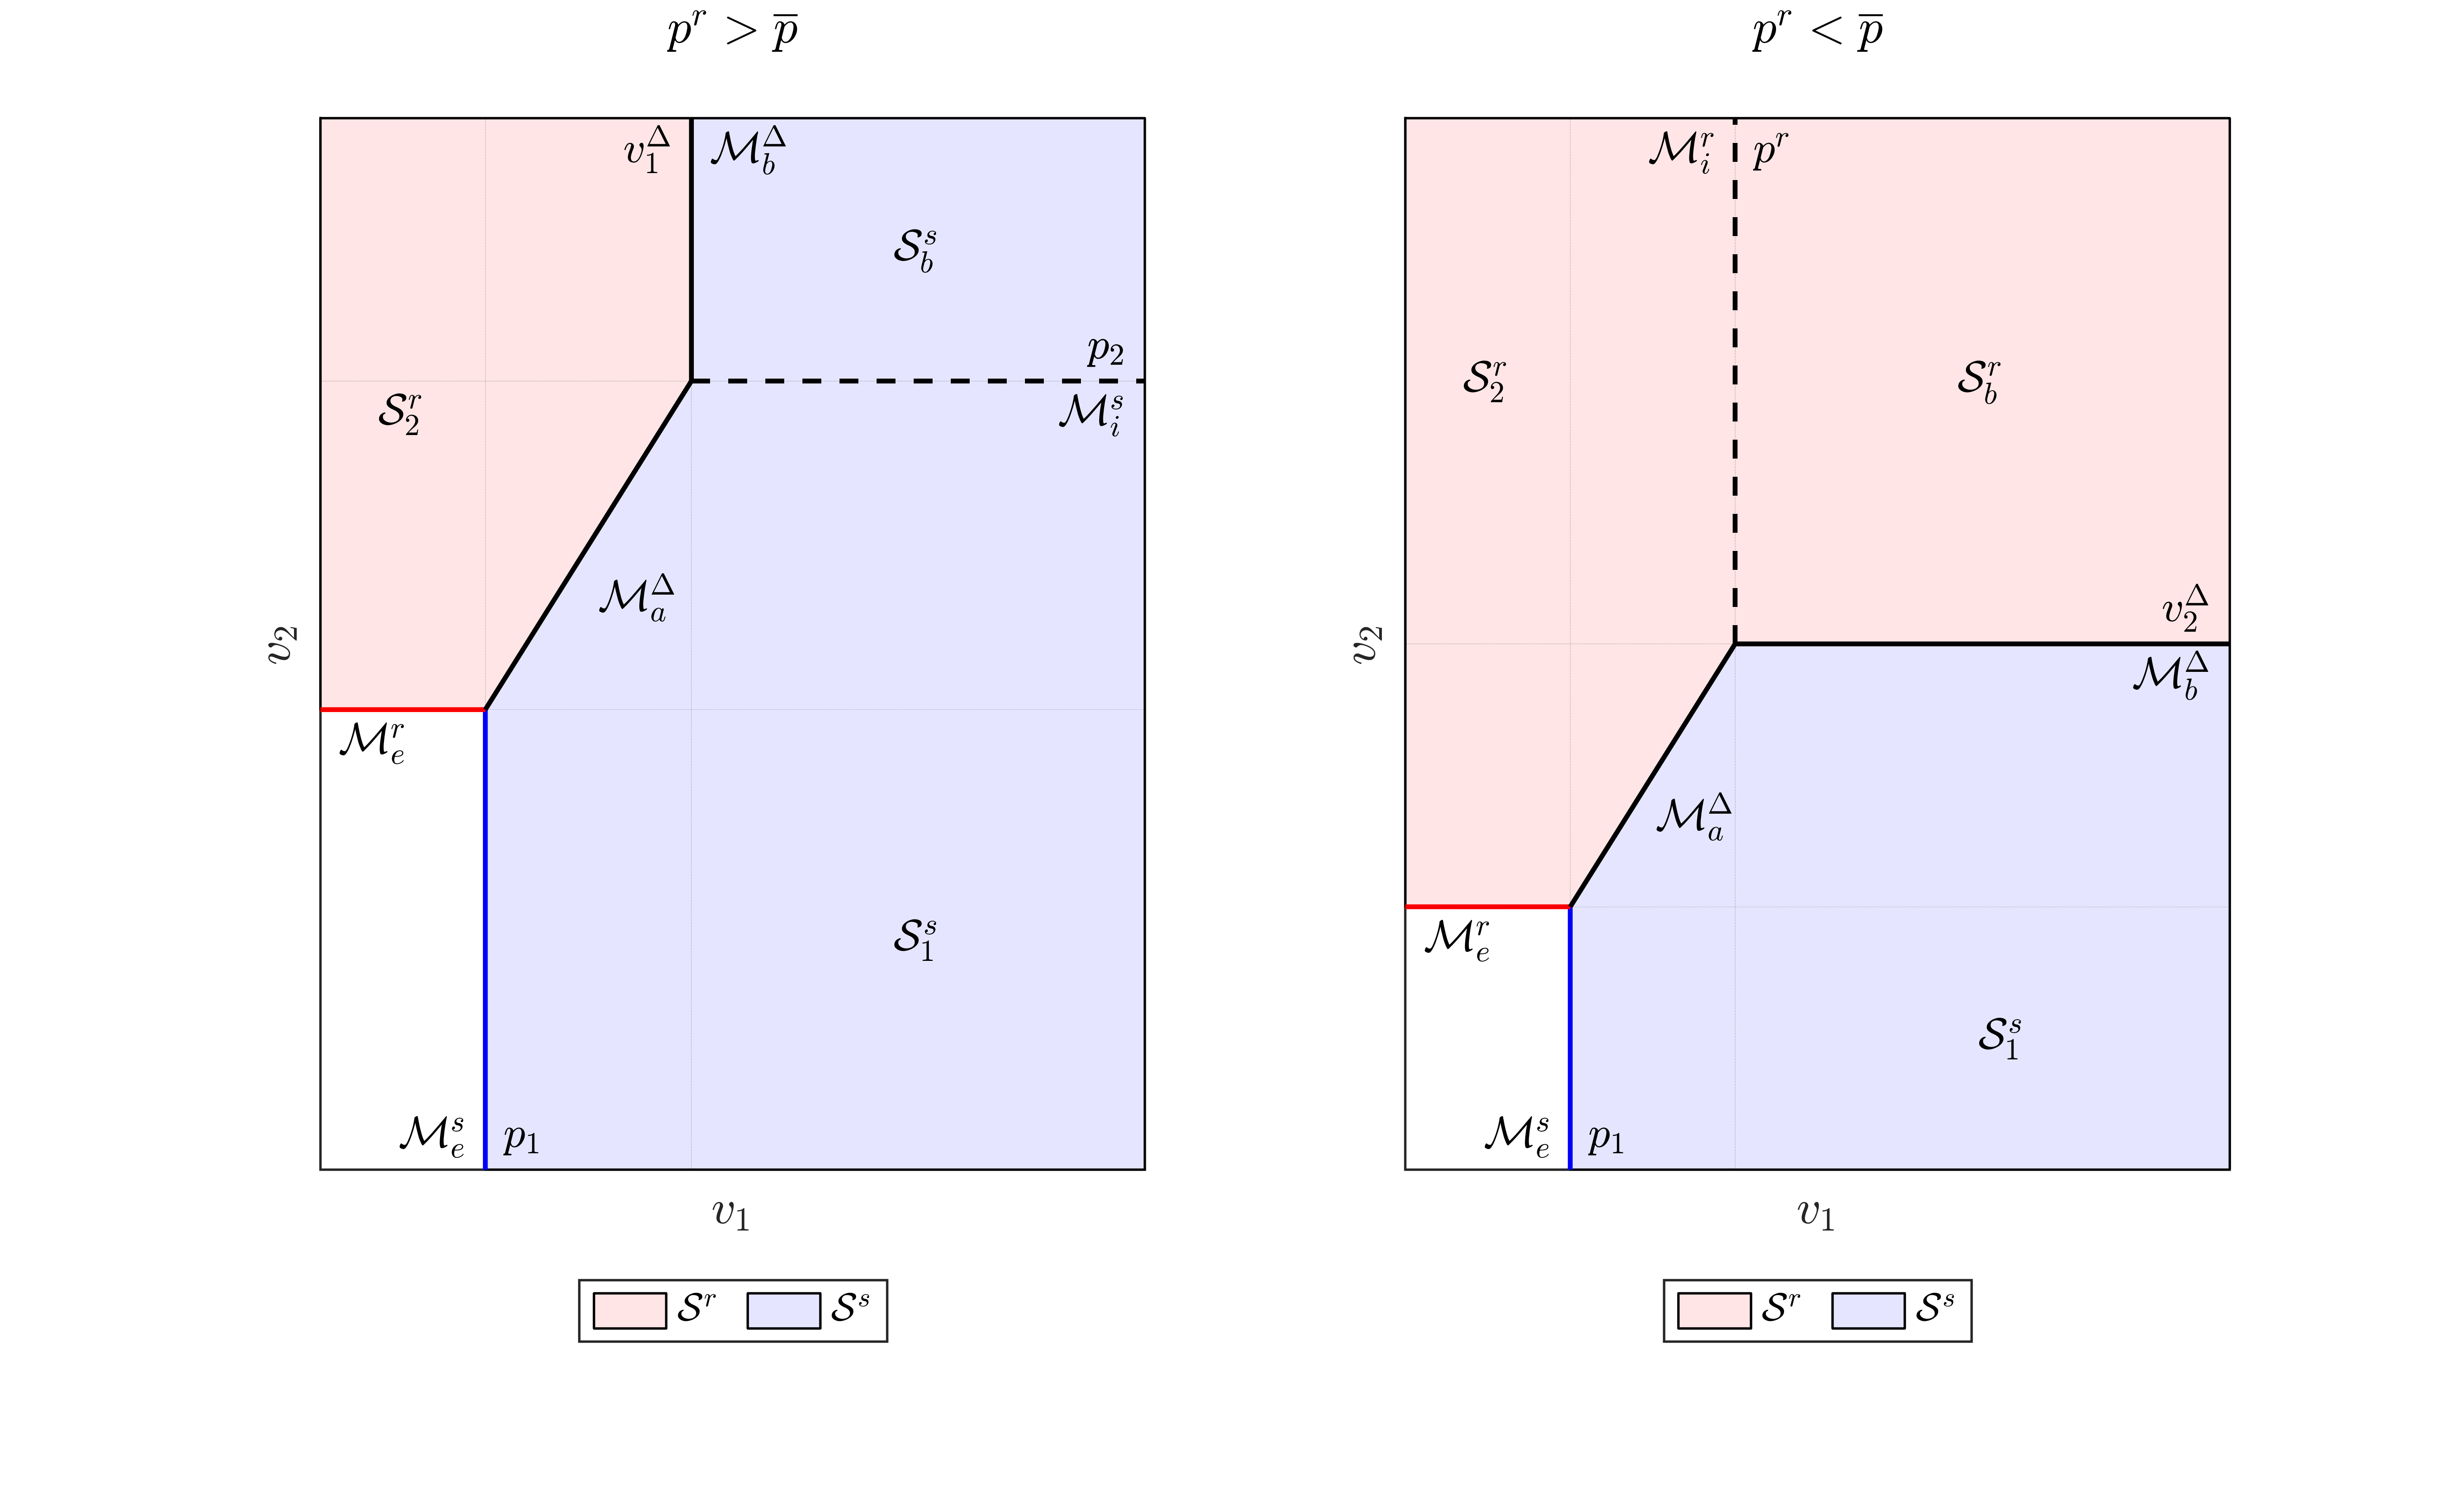
\includegraphics[width=1\linewidth]{figure/example_conv_cstc.png}
     \caption{The set of \textit{contract switchers} defines the mass of consumers choosing each contract.             \hyperlink{demand2}{\beamerreturnbutton{Demand}}}
\end{figure}
    
\end{frame}


%%%%%%%%%%%%%%%%%%%%%%%%%%%%%%%%%%%%%%%%%%%%%%%%%%%%%%%%%%%%%%%%%%%%%%%%%%%%%%%%%%%%%%%%%%%%%%%%%%%%%%%%%%%%%%%%%%%%%%%%%%%%%%%%%%%%%%%%%%%%%%%%%%%%%%
%%%%%%%%%%%%%%%%%%%%%%%%%%%%%%%%%%%%%%%%%%%%%%%%%%%%%%%%%%%%%%%%%%%%%%%%%%%%%%%%%%%%%%%%%%%%%%%%%%%%%%%%%%%%%%%%%%%%%%%%%%%%%%%%%%%%%%%%%%%%%%%%%%%%%%
%%%%%%%%%%%%%%%%%%%%%%%%%%%%%%%%%%%%%%%%%%%%%%%%%%%%%%%%%%%%%%%%%%%%%%%%%%%%%%%%%%%%%%%%%%%%%%%%%%%%%%%%%%%%%%%%%%%%%%%%%%%%%%%%%%%%%%%%%%%%%%%%%%%%%%

\section{General equilibrium}

\begin{frame}{Roadmap}
  \tableofcontents [sectionstyle=show/shaded,subsectionstyle=show/shaded]
\end{frame}

\subsection{Incentives for a fixed-price contract}

%%%%%%%%%%%%%%%%%%%%%%%%%%%%%%%%%%%%%%%%%%%%%%%%%%%%%%%%%%%%%%%%%%%%%%%%%%%%%%%%%%%%%%%%%%%%%%%%%%%%%%%%%%%%%%%%%%%%%%%%%%%%%%%%%%%%%%%%%%%%%%%%%%%%%%


\begin{frame}{Entry of a fixed-price contract}

\begin{figure}
    \centering
    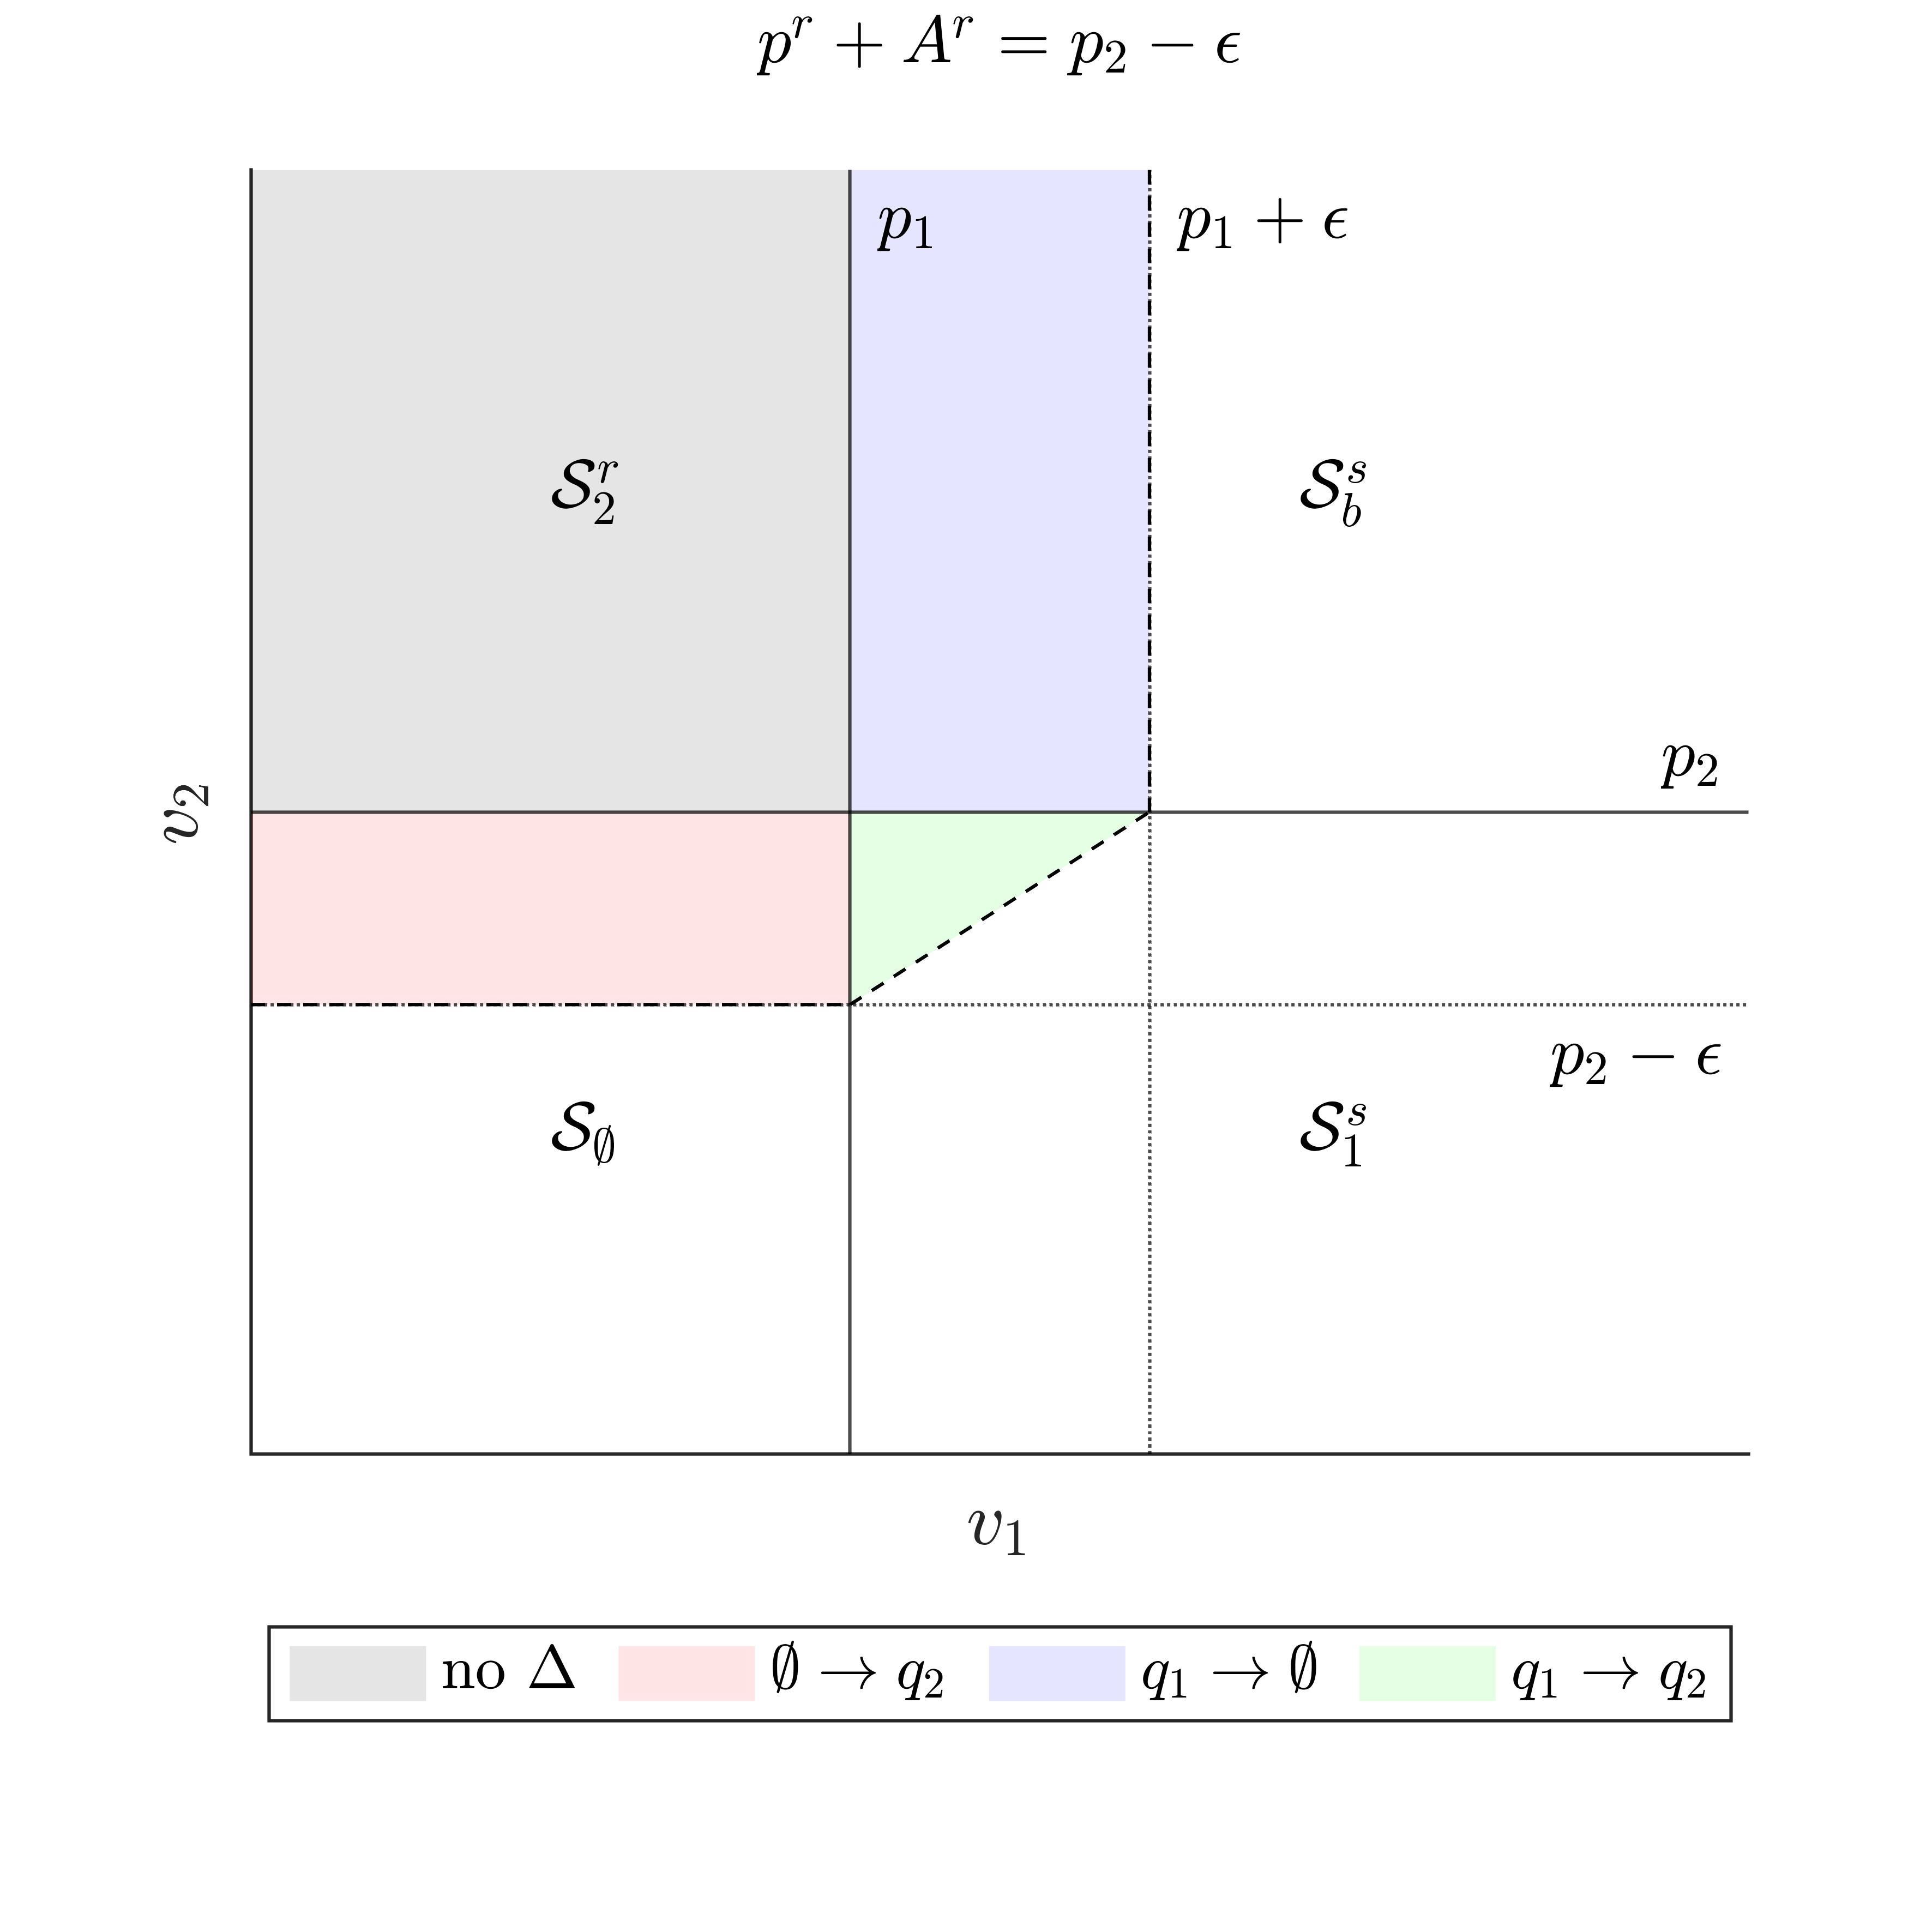
\includegraphics[width=0.65\linewidth]{figure/spot_demand_multi_sb_ppt.png}
    \caption{Downward price deviation of the fixed price with entry.}
    \label{fig:spot_demand_multi_sb_ppt}
\end{figure}
    
\end{frame}

%%%%%%%%%%%%%%%%%%%%%%%%%%%%%%%%%%%%%%%%%%%%%%%%%%%%%%%%%%%%%%%%%%%%%%%%%%%%%%%%%%%%%%%%%%%%%%%%%%%%%%%%%%%%%%%%%%%%%%%%%%%%%%%%%%%%%%%%%%%%%%%%%%%%%%

\subsection{Private Firms Equilibrium}


\begin{frame}{Private Firms Equilibrium}

\begin{proposition}
The unit-price equilibrium of the RTP contract $\textbf{p}^s$ is at the marginal cost: $p_t = c_t \ \forall t$ and $A^s = 0$.
\end{proposition}

\begin{proposition}
A mixed-equilibrium contract in which consumers have a strict preference for an FP contract offered by either \boldrblue{a private firm} does not exist. 
\end{proposition}

\vfill

\begin{itemize}
    \item \textbf{RTP contract}: Bertrand Competition \vfill
    \item \textbf{FP contract}: Market unraveling  \vfill

\begin{itemize}
    \item \boldrblue{The demand and the average cost} of the FP contract depend on the RTP prices  which are set at $p_t=c_t$. \vfill

\item Then  $  \quad  \nexists p^r
    \quad \text{s.t.} \quad
    p^r=AC^r(p^r;p_1,p_2)
    \quad \text{and} \quad
    q^r(p^r;p_1,p_2)>0$.\vfill

\end{itemize}




\end{itemize}

\end{frame}
% 
%%%%%%%%%%%%%%%%%%%%%%%%%%%%%%%%%%%%%%%%%%%%%%%%%%%%%%%%%%%%%%%%%%%%%%%%%%%%%%%%%%%%%%%%%%%%%%%%%%%%%%%%%%%%%%%%%%%%%%%%%%%%%%%%%%%%%%%%%%%%%%%%%%%%%%


\begin{frame}{Market unraveling of the fixed-price market} \label{PrivateFirms2}


\begin{figure}
    \centering
    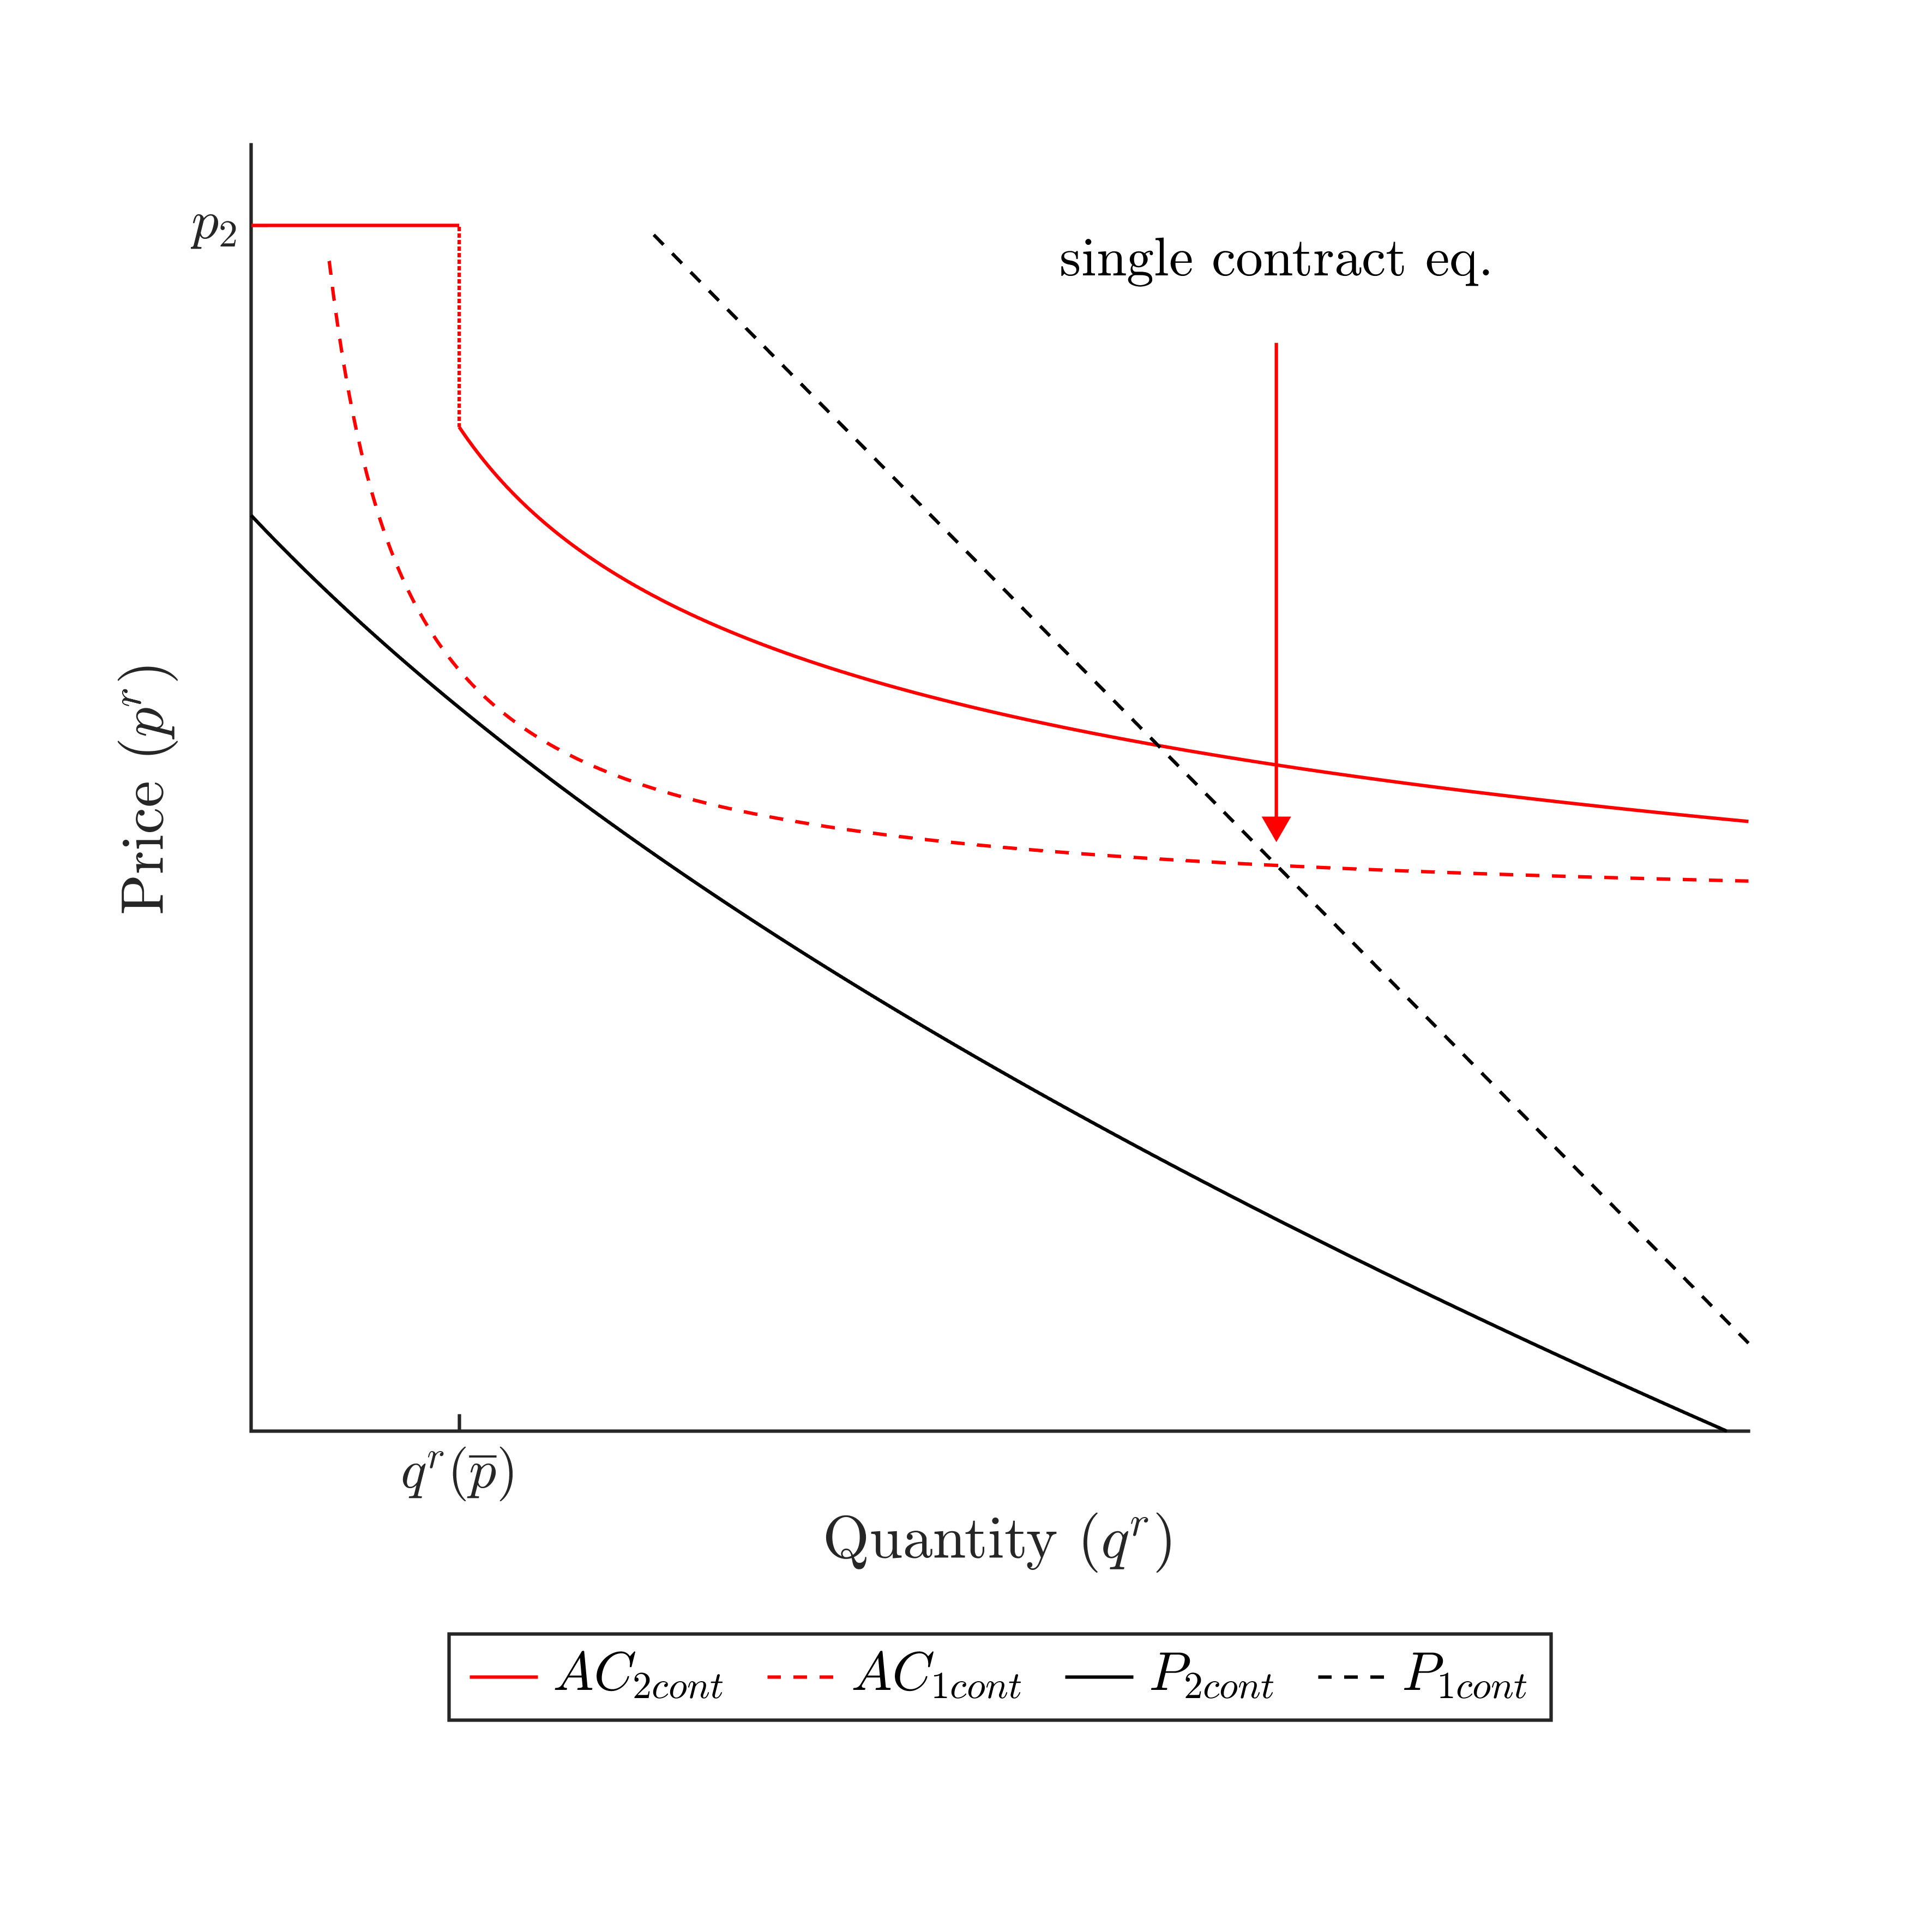
\includegraphics[width=0.75\linewidth]{figure/Exemple_Private_u_ddeAC_ppt.png}
\end{figure}
    
\end{frame}
% % 
% %%%%%%%%%%%%%%%%%%%%%%%%%%%%%%%%%%%%%%%%%%%%%%%%%%%%%%%%%%%%%%%%%%%%%%%%%%%%%%%%%%%%%%%%%%%%%%%%%%%%%%%%%%%%%%%%%%%%%%%%%%%%%%%%%%%%%%%%%%%%%%%%%%%%%%

% \begin{frame}{Self financing public firm}

% \begin{itemize}
% \item We consider a self-financing \textit{public firm}. It offers the fixed-price contract and chooses $(p^r,A^r)$ to maximize consumer surplus subject to breaking even:

% \vfill

% \begin{align*}  
%     (p^r,A^r) \quad & \in \quad  
%     \arg\max_{p^r,A^r}
%     CS^r(p^r,A^r) \\\\
%     &\text{s.t.} \quad
%     \pi^r(p^r,A^r)=0.
% \end{align*}


% \vfill


% \begin{lemma}\label{lem:tax}
% With a public firm and a full self-financing levy, there is no mixed-equilibrium contract in which consumers have a strict preference for an FP contract offered by the public firm. 
% \end{lemma}
% \end{itemize}


% \end{frame}

\subsection{Public Firm Equilibrium}

\begin{frame}{Roadmap}
  \tableofcontents [sectionstyle=show/shaded,subsectionstyle=show/shaded]
\end{frame}



%%%%%%%%%%%%%%%%%%%%%%%%%%%%%%%%%%%%%%%%%%%%%%%%%%%%%%%%%%%%%%%%%%%%%%%%%%%%%%%%%%%%%%%%%%%%%%%%%%%%%%%%%%%%%%%%%%%%%%%%%%%%%%%%%%%%%%%%%%%%%%%%%%%%%%
\begin{frame}{Publicly-funded Regulated Firm Equilibrium - Existence}\label{ProgramMain}


\begin{itemize}
    \item General form:
\end{itemize}

\[  \Omega^r(p^r,A^r)
    =
    CS^r(p^r,A^r)
    + (1+\lambda) \pi^r(p^r,A^r)\]

 \vfill

   \hyperlink{ProgramExtension}{\beamerreturnbutton{ Self-financing and  Market-wide tax Extension}}
   
  \vfill
 
 
\begin{itemize}
    \item Recall $\mathcal{M}^\Delta_{a,b}$ is the set of contract switchers and $q_2^r(p_2)$ the quantity consumed in period 2.
\end{itemize}

 \vfill

\begin{proposition}\label{prop:sufficientcod}
A public firm has a strict incentive to offer a fixed price contract iff: 

\begin{equation*}
    \underbrace{\Bigg. \int_{\M^\Delta_{a,b}|_{\epsilon = 0^+}} (v_2 - p_2) f_1(p_1 ) f_2(v_2 ) dv_2\Bigg.  }_{\text{marginal benefit}} > \underbrace{\Bigg. \lambda q^r|_{\epsilon = 0^+}\Bigg. }_{\text{inframarginal cost}}  \label{con_exi_FP}
\end{equation*}

\end{proposition}

\end{frame}


%%%%%%%%%%%%%%%%%%%%%%%%%%%%%%%%%%%%%%%%%%%%%%%%%%%%%%%%%%%%%%%%%%%%%%%%%%%%%%%%%%%%%%%%%%%%%%%%%%%%%%%%%%%%%%%%%%%%%%%%%%%%%%%%%%%%%%%%%%%%%%%%%%%%%%

\begin{frame}{Incentive for fixed-price contract}

\begin{figure}
    \centering
    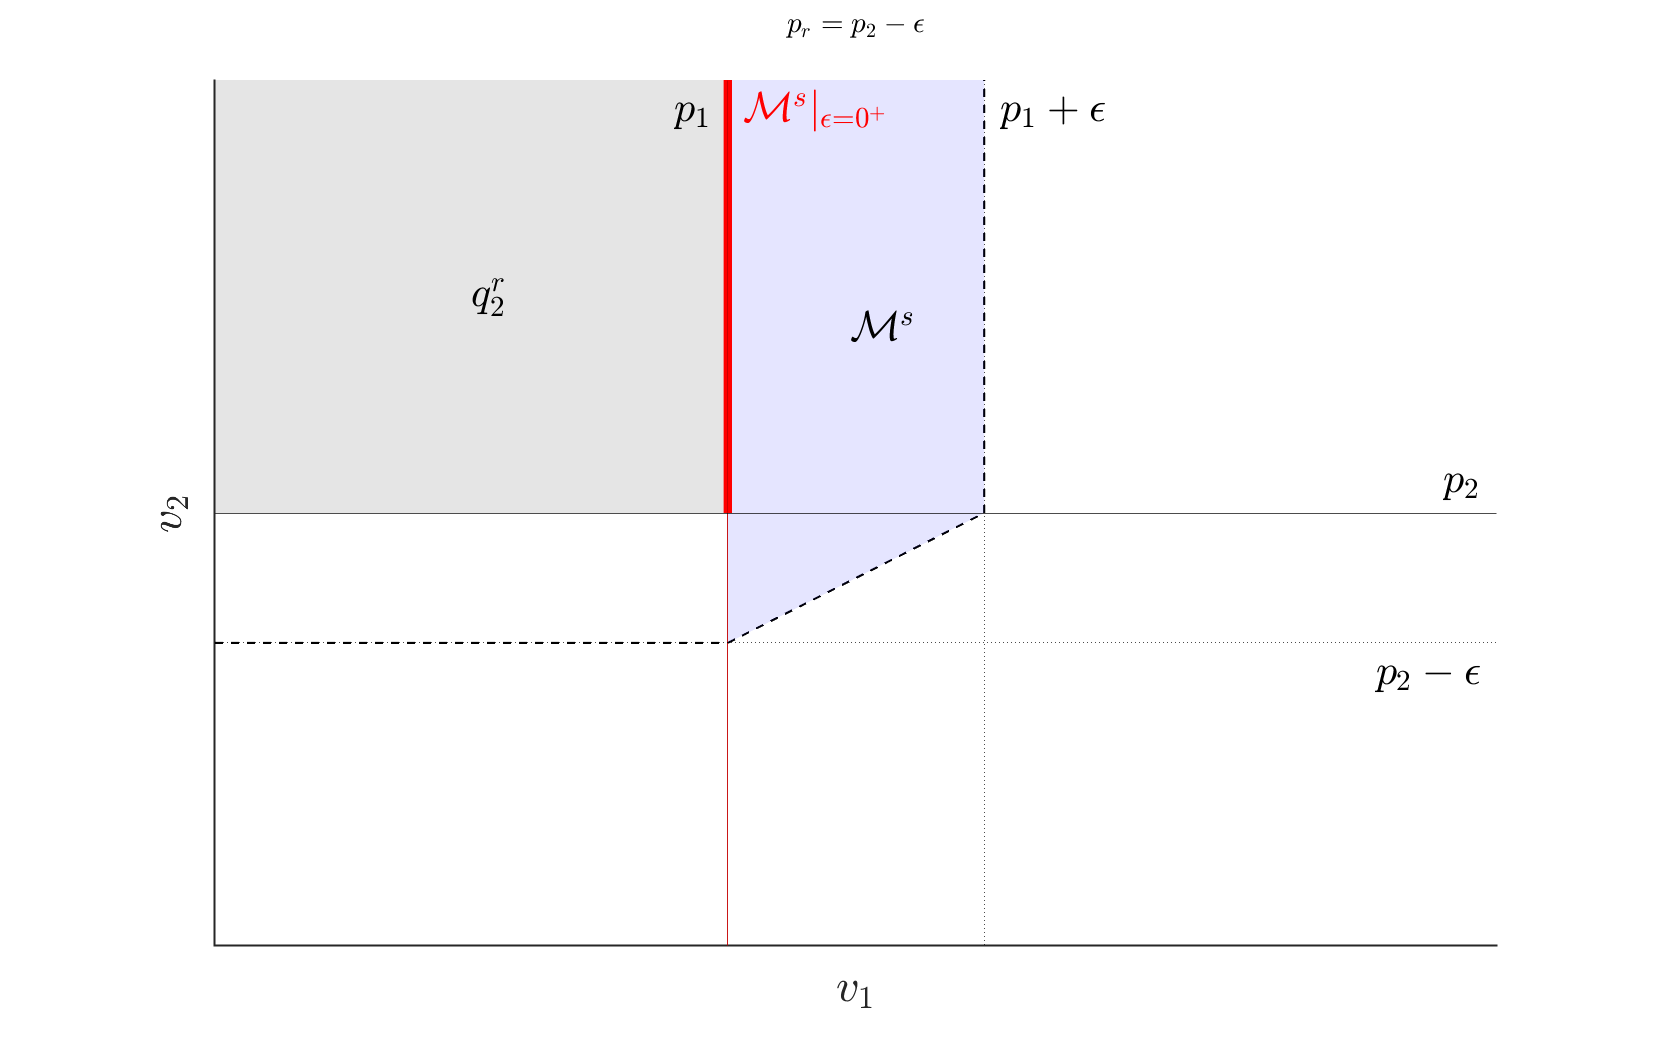
\includegraphics[width=1\linewidth]{figure/spot_demand_multi_sb_ppt_equil.png}
    \caption{Tradeoff for profitability of the public fixed-price contract.}
    \label{fig:spot_demand_multi_sb_ppt_equil}
\end{figure}
    
\end{frame}

%%%%%%%%%%%%%%%%%%%%%%%%%%%%%%%%%%%%%%%%%%%%%%%%%%%%%%%%%%%%%%%%%%%%%%%%%%%%%%%%%%%%%%%%%%%%%%%%%%%%%%%%%%%%%%%%%%%%%%%%%%%%%%%%%%%%%%%%%%%%%%%%%%%%%%



\begin{frame}{Marginal responses - Illustration}

    \begin{figure}
    \centering
    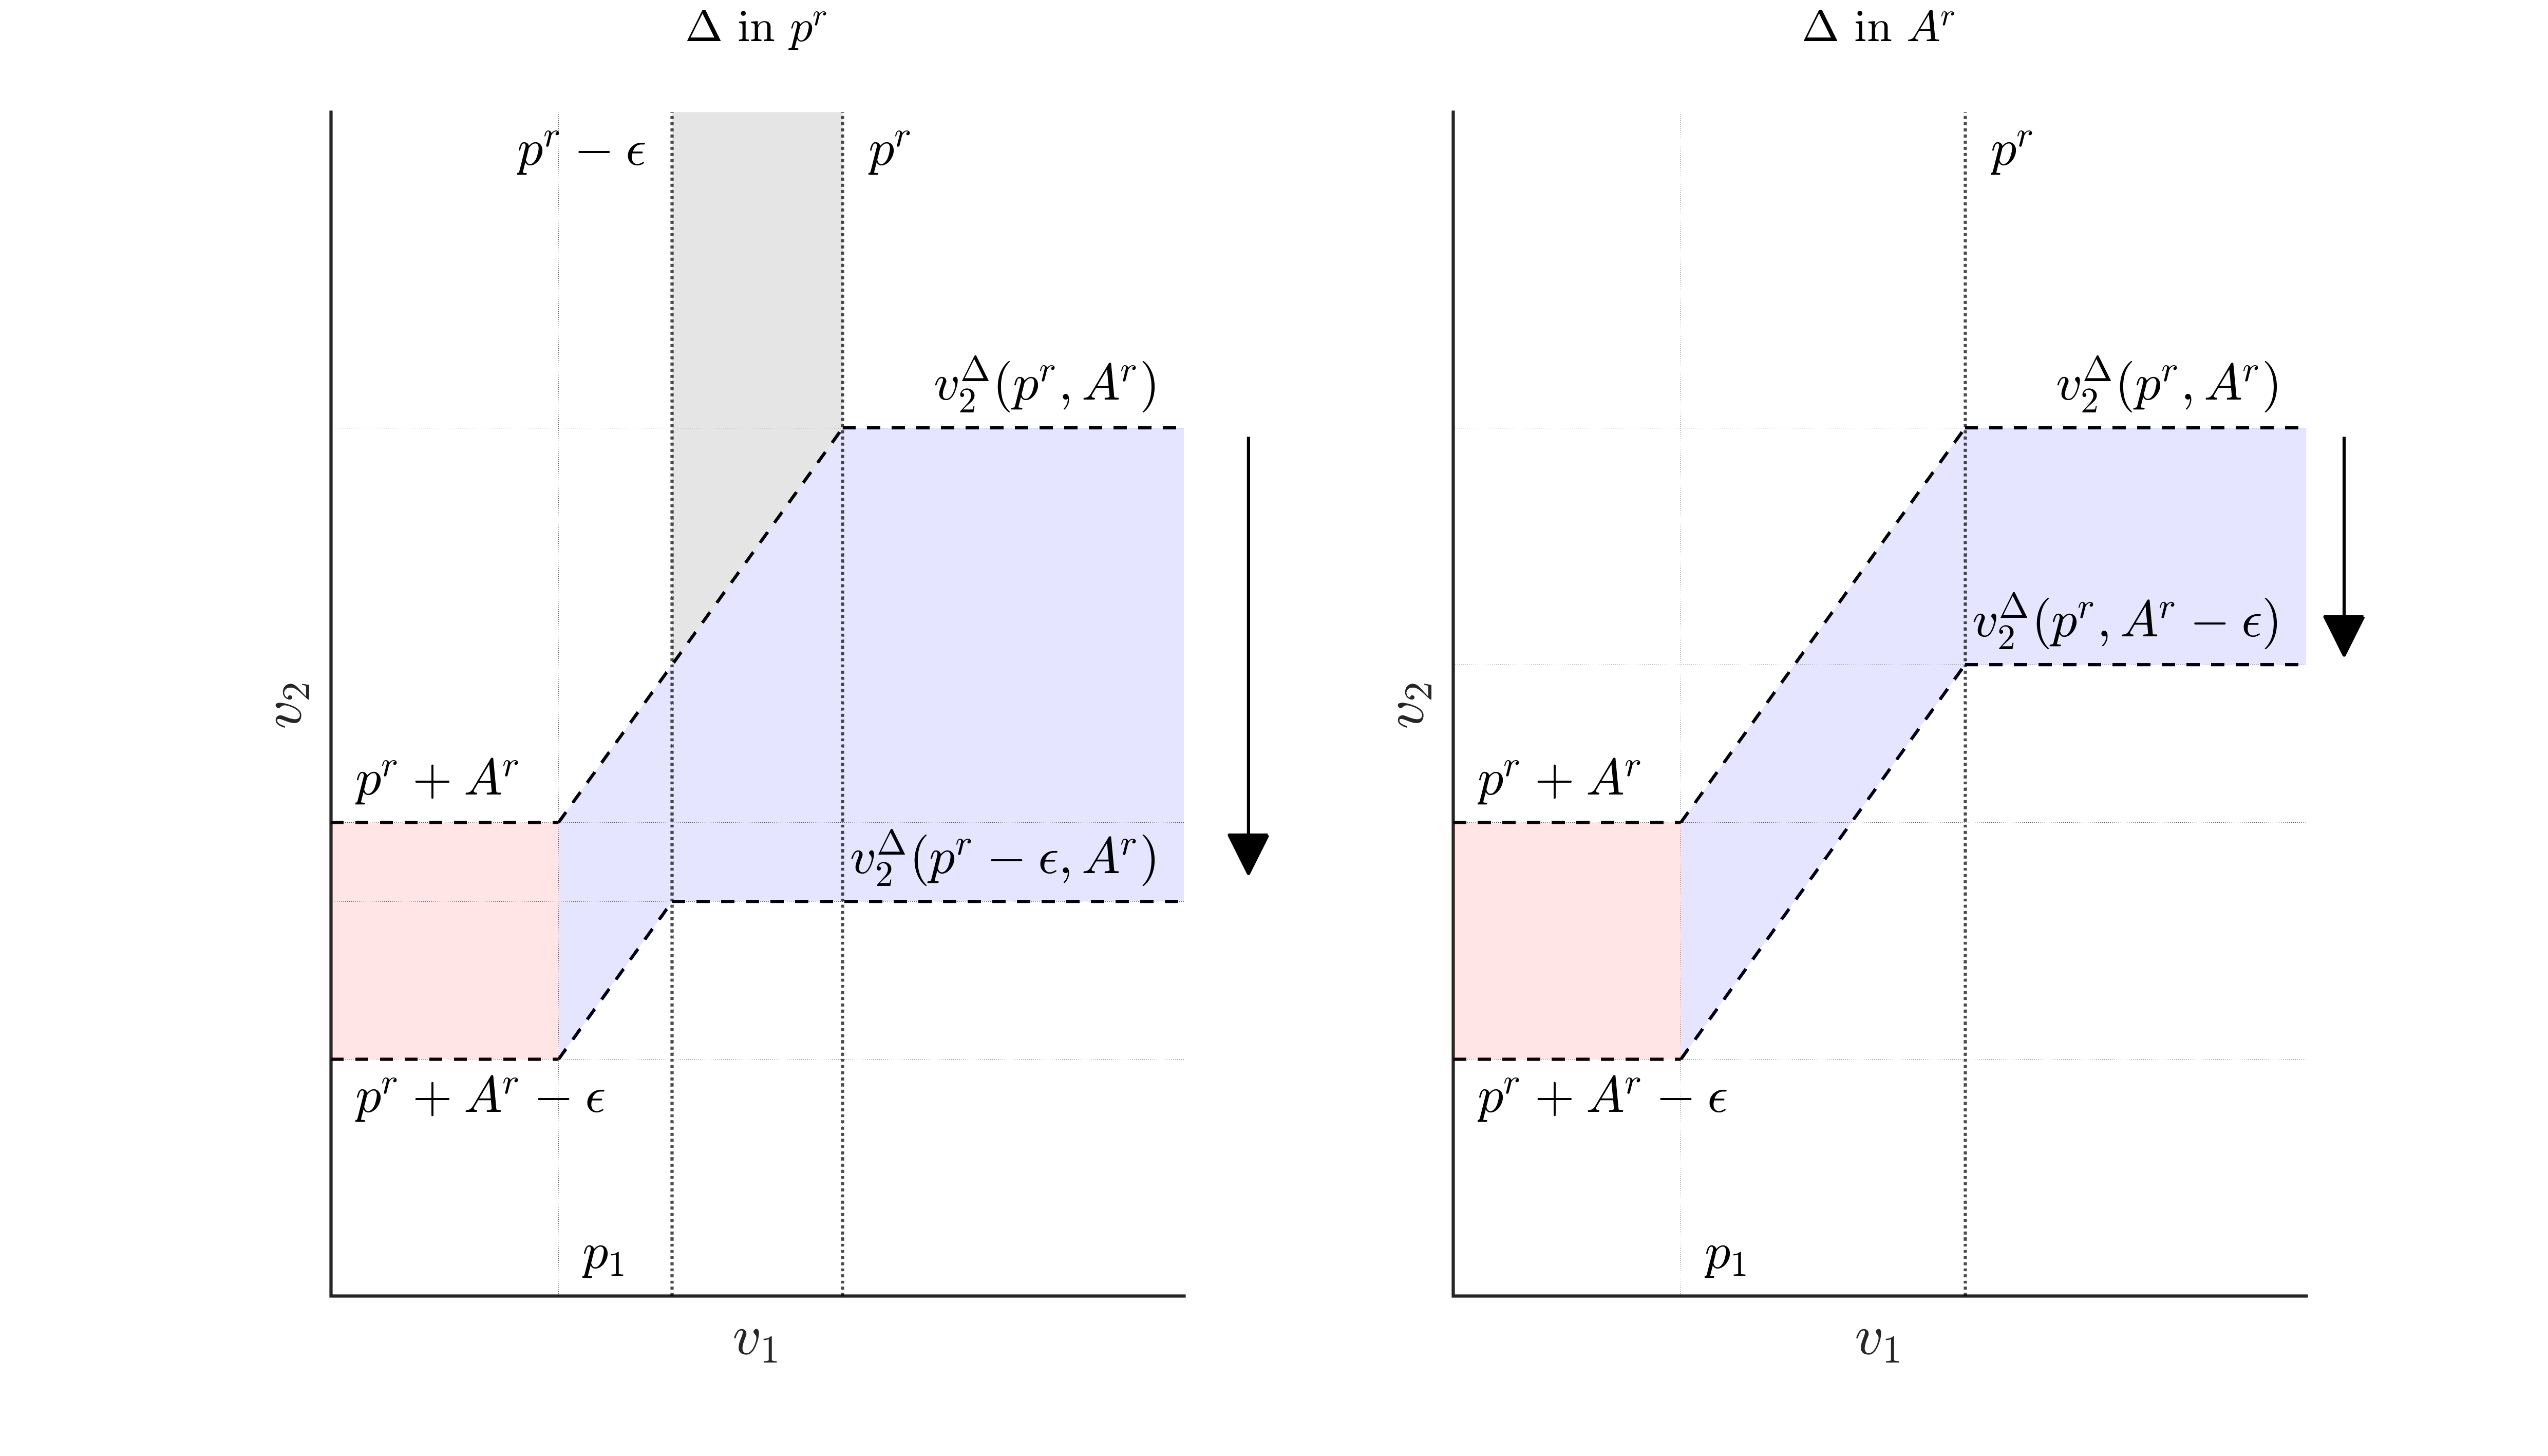
\includegraphics[width=1\linewidth]{figure/spot_demand_v2_sb_ppt.png}
    \caption{Change in consumption and contract choice after an equal deviation in the unit price $p^r$ (left) and in the fixed part $A^r$ (right). The gray zone indicates profile switchers. Blue zones indicate contract switchers. Red zones indicate exiters.}
    \label{fig:spot_demand_v2_sb_ppt}
\end{figure}

\end{frame}

%%%%%%%%%%%%%%%%%%%%%%%%%%%%%%%%%%%%%%%%%%%%%%%%%%%%%%%%%%%%%%%%%%%%%%%%%%%%%%%%%%%%%%%%%%%%%%%%%%%%%%%%%%%%%%%%%%%%%%%%%%%%%%%%%%%%%%%%%%%%%%%%%%%%%%

\begin{frame}{Marginal responses}

\small

The difference in \boldrblue{marginal quantity responses} between $A^r$ and $p^r$

\vfill

\[
\delta_{A}(X) \;:=\; \frac{\partial X}{\partial A^r} \;-\; \frac{\partial X}{\partial p^r},
\]


\vfill

The \boldrblue{consumer surplus  of contract switchers}: 

\begin{align*}
\partial_{p^r}\mathcal{C} :=  - \overbrace{\frac{\partial \phi(v_1)}{\partial p^r} \int_{\M^\Delta_{a}} (\phi(v_1) - p^r-A^r) f_1(v_1) f_2(\phi(v_1))dv_1}^{\text{sorting effect \#1}}  \\
- \underbrace{\frac{\partial v_2^\Delta}{\partial p^r} \int_{\M^\Delta_b} ( v_2^\Delta - p^r-A^r) f_1(v_1) f_2(v_2^\Delta) dv_1}_{\text{sorting effect \#2}}    
\end{align*}

\footnotesize
where $\phi(v_1)$ and $v_2^\Delta$ characterize the set of marginal consumers' WTP.

\end{frame}

%%%%%%%%%%%%%%%%%%%%%%%%%%%%%%%%%%%%%%%%%%%%%%%%%%%%%%%%%%%%%%%%%%%%%%%%%%%%%%%%%%%%%%%%%%%%%%%%%%%%%%%%%%%%%%%%%%%%%%%%%%%%%%%%%%%%%%%%%%%%%%%%%%%%%%

\begin{frame}{Equilibrium}\label{RamseyOutside}


\begin{proposition}\label{prop:eqFPPublic}
If an interior equilibrium with $p^r<\overline{p}$ exists, the unit price $p^r$ and fixed part $A^r$ of the FP contract offered by the public firm satisfy

\vspace{0.25 cm}

\begin{equation*}
p^r_{\ast \ast}
\;=\;
\underbrace{\sum_{t} c_t\,\frac{\delta_{A}(q_t^r)}{\delta_{A}(q^r)}}_{\text{marginal cost}} \; + \; \text{Two-part Ramsey term}
\;-\;
\underbrace{\frac{1}{1+\lambda}\,\frac{\delta_{A}(\mathcal{C})}{\delta_{A}(q^r)}}_{\text{sorting correction}}
\end{equation*}

\vspace{0.25 cm}

If an interior equilibrium with $p^r>\overline{p}$ exists, the unit price $p^r$ of the FP contract offered by the public firm satisfies

\vspace{0.25 cm}

\[
p^r_{\ast \ast} \;=\; c_2  \; + \;
\text{Two-part Ramsey term}
\;-\;
\underbrace{\frac{1}{1+\lambda}\,\frac{\partial_{p^r}\mathcal{C}}{\partial_{p^r}(q^r_2)}}_{\text{sorting correction}}.
\]

\end{proposition}


\boldrblue{Where}  $\delta_{A}(\cdot)>0$ and $\partial_{p^r}(\cdot)<0 \qquad $    \hyperlink{Ramseytax}{\beamerreturnbutton{Market-wide tax Equilibrium}}



\end{frame}



%%%%%%%%%%%%%%%%%%%%%%%%%%%%%%%%%%%%%%%%%%%%%%%%%%%%%%%%%%%%%%%%%%%%%%%%%%%%%%%%%%%%%%%%%%%%%%%%%%%%%%%%%%%%%%%%%%%%%%%%%%%%%%%%%%%%%%%%%%%%%%%%%%%%%%

\section{Welfare Implications}

%%%%%%%%%%%%%%%%%%%%%%%%%%%%%%%%%%%%%%%%%%%%%%%%%%%%%%%%%%%%%%%%%%%%%%%%%%%%%%%%%%%%%%%%%%%%%%%%%%%%%%%%%%%%%%%%%%%%%%%%%%%%%%%%%%%%%%%%%%%%%%%%%%%%%%

\begin{frame}{Roadmap}
  \tableofcontents [sectionstyle=show/shaded,subsectionstyle=show/shaded]
\end{frame}

%%%%%%%%%%%%%%%%%%%%%%%%%%%%%%%%%%%%%%%%%%%%%%%%%%%%%%%%%%%%%%%%%%%%%%%%%%%%%%%%%%%%%%%%%%%%%%%%%%%%%%%%%%%%%%%%%%%%%%%%%%%%%%%%%%%%%%%%%%%%%%%%%%%%%%

\begin{frame}{Welfare comparison}


\begin{itemize}
   
    \item Private firms: \boldrblue{ First-Best}. \vfill

    \item Public Firm + Private Firms + Consumer Choices \boldrblue{?} \vfill

    \item We compare the welfare with \boldrblue{a single contract} environment. \vfill

    \begin{itemize}
        \item We show that the \boldrblue{welfare can be ambiguous}. \vfill
        \item This is notably due to having \boldrblue{a lower fixed-price} compared to the single contract case. \vfill
    \end{itemize}



\begin{center}
    W(\textcolor{blue}{Dynamic}: $p_t = c_t$ +  \textcolor{red}{Fixed-Price}: $p^r=p^r_{\ast \ast}$)  { \textbf{  < }} $W$( \textcolor{red}{Fixed-Price}: $p_{fp}^r$)
\end{center}

\vfill

Where $p_{fp}^r$ is the equilibrium price set by the public firm in the single contract benchmark (Ramsey price).

    
\end{itemize}
    
\end{frame}


%%%%%%%%%%%%%%%%%%%%%%%%%%%%%%%%%%%%%%%%%%%%%%%%%%%%%%%%%%%%%%%%%%%%%%%%%%%%%%%%%%%%%%%%%%%%%%%%%%%%%%%%%%%%%%%%%%%%%%%%%%%%%%%%%%%%%%%%%%%%%%%%%%%%%%

\begin{frame}{Equilibrium comparison}

\begin{figure}
    \centering
    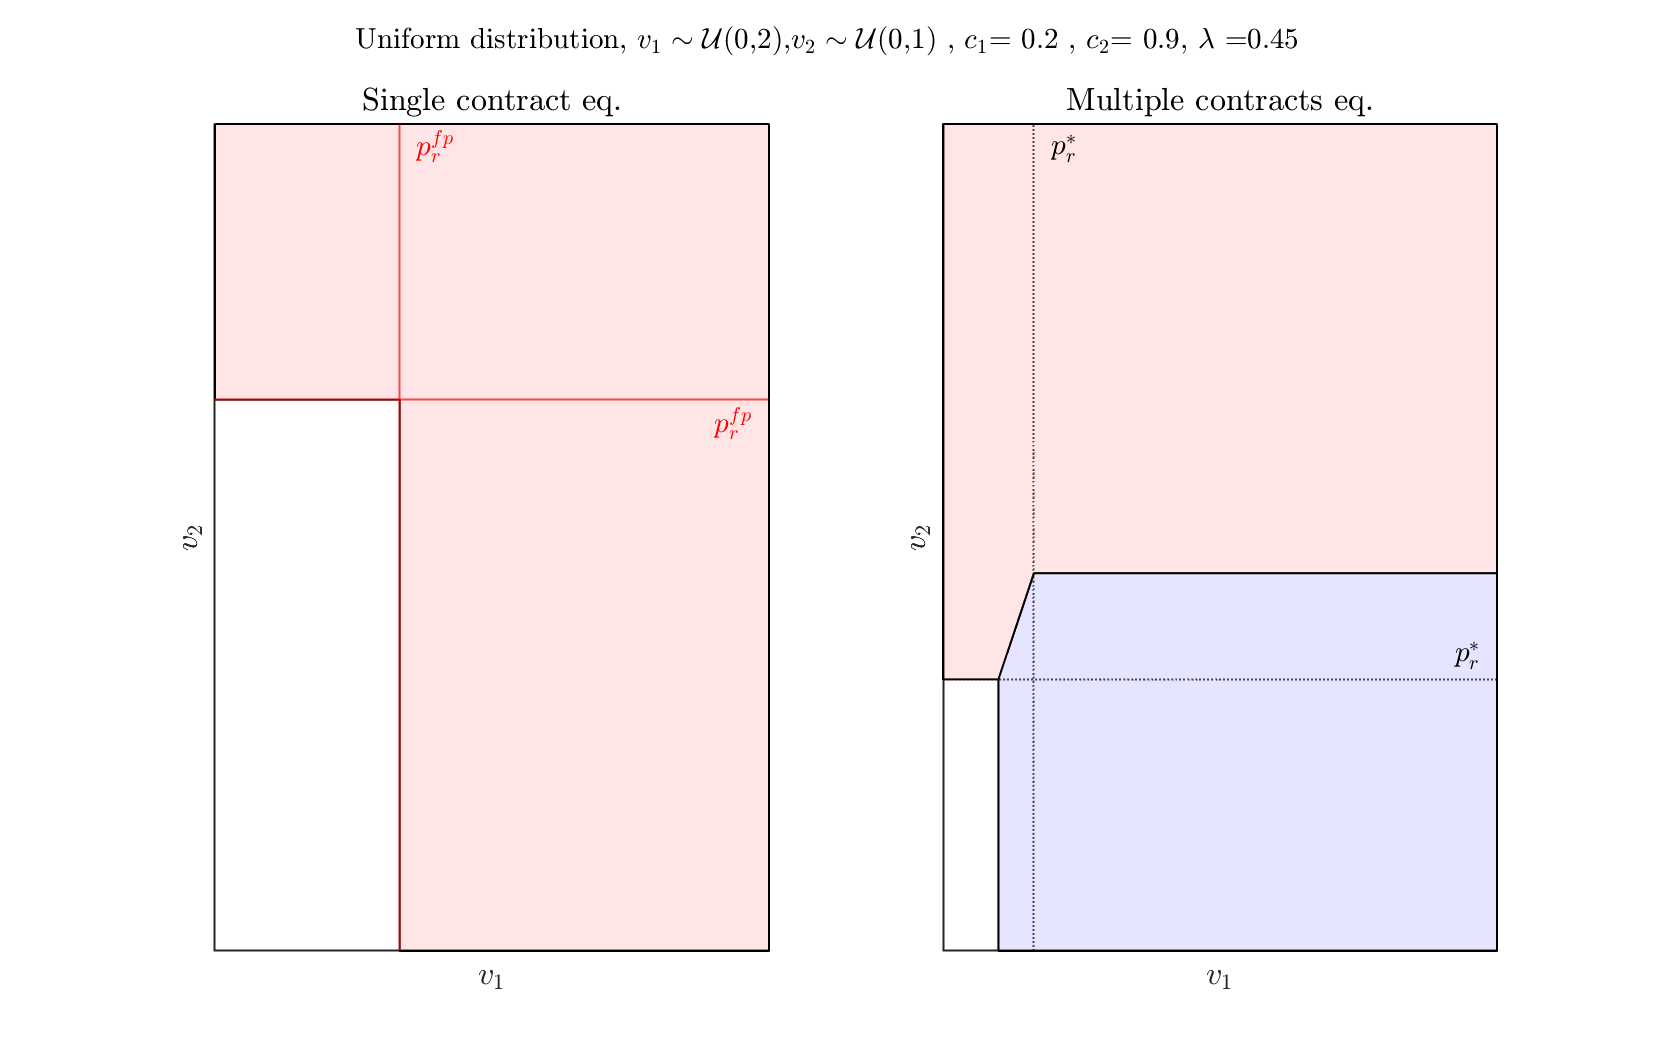
\includegraphics[width=0.95\linewidth]{figure/example_equ1_u.png}
\end{figure}
    
\end{frame}



%%%%%%%%%%%%%%%%%%%%%%%%%%%%%%%%%%%%%%%%%%%%%%%%%%%%%%%%%%%%%%%%%%%%%%%%%%%%%%%%%%%%%%%%%%%%%%%%%%%%%%%%%%%%%%%%%%%%%%%%%%%%%%%%%%%%%%%%%%%%%%%%%%%%%%

\begin{frame}{Self-Selection Equilibrium vs. S.B. Linear Pricing FP Contract }

\small 

Change in deadweight loss between the two equilibrium

\vfill
\[
\begin{aligned}
    \Delta DW
\;=\;
\Delta DW^{s}(\text{selection RTP})
\;+\;
\Delta DW^{r}_{1}(t_1 \text{misalloc.})
+\;
\Delta DW^{r}_{2}(t_2 \text{misalloc.}),
\end{aligned}
\]

\begin{figure}[!ht]
 \centering
 \makebox[\textwidth][c]{%
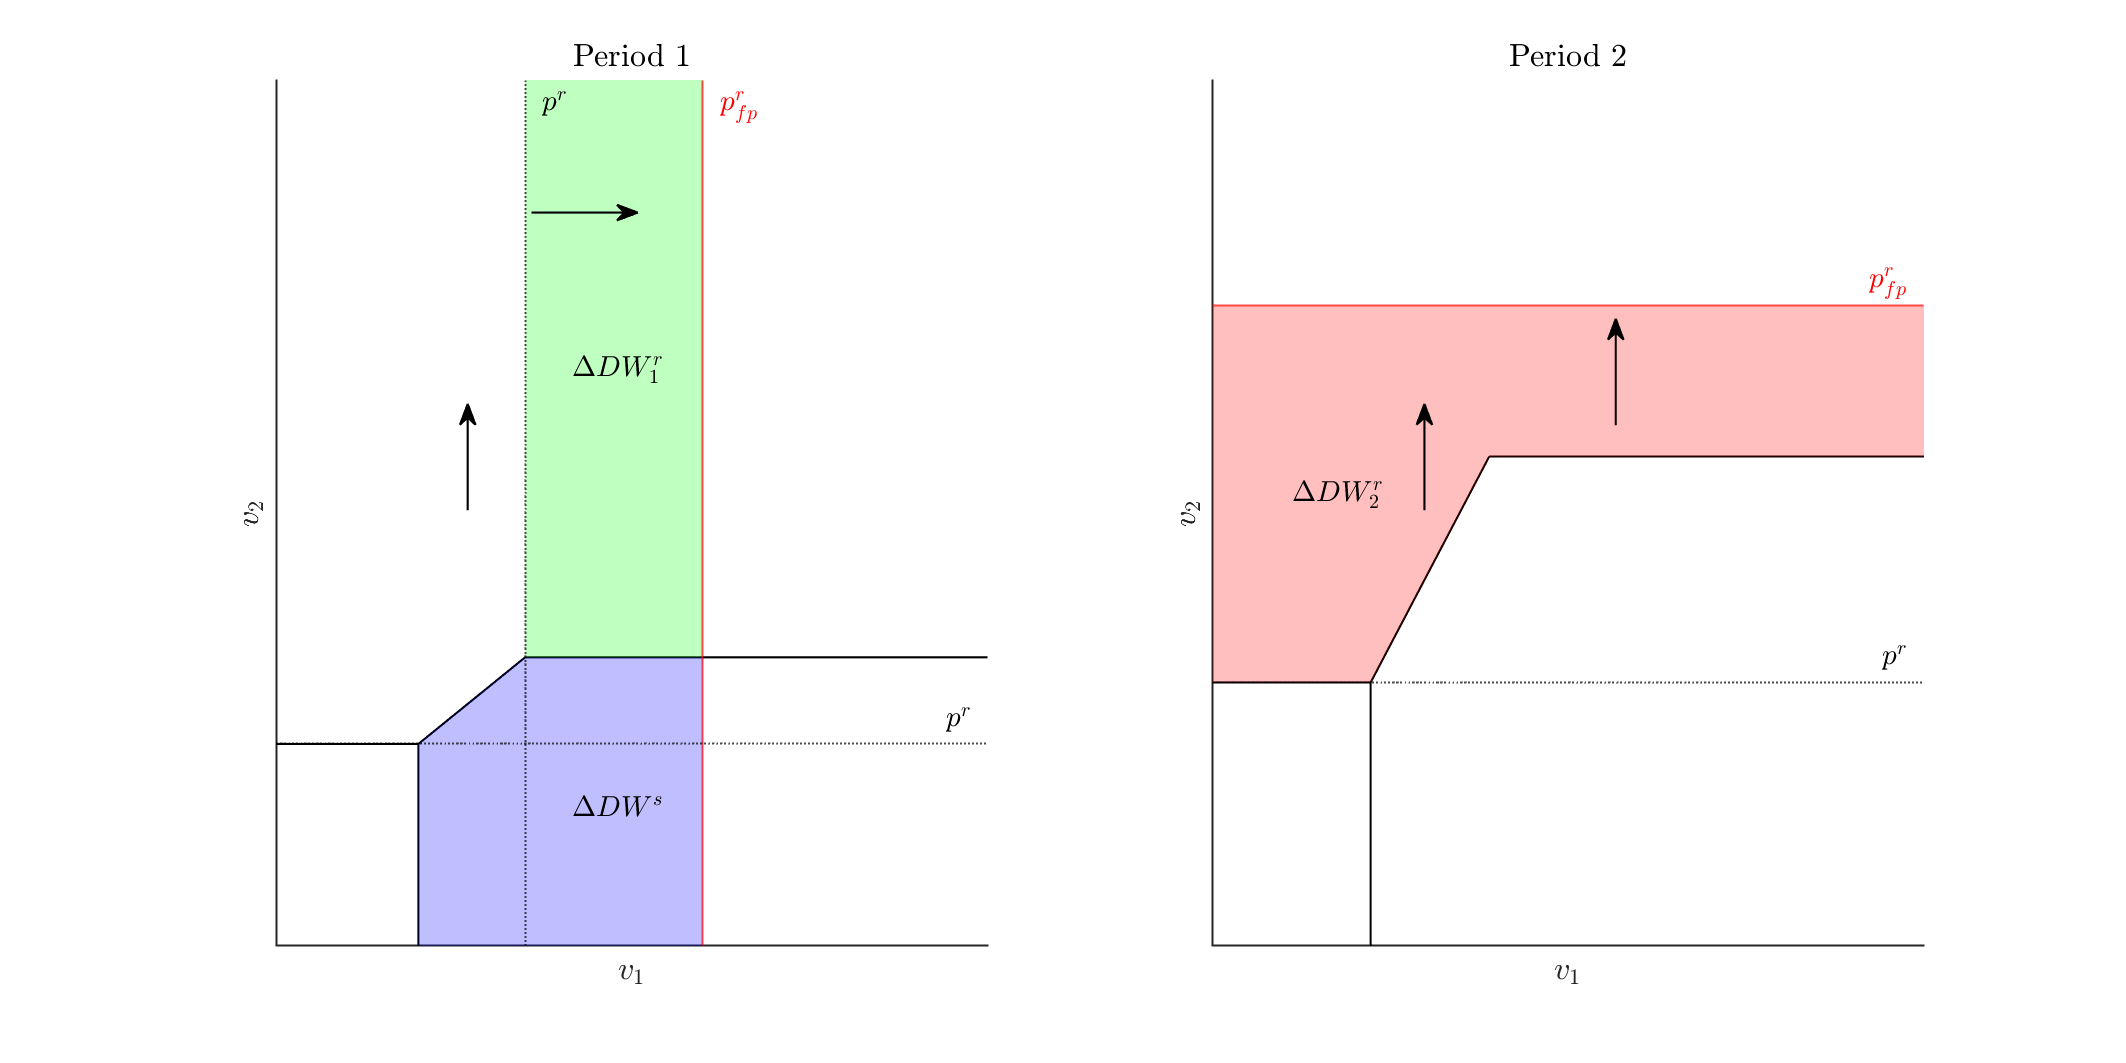
\includegraphics[width=0.95\linewidth]{figure/ExampleSurplusCUNIF.png}
 }
 \caption{Comparison of welfare change between the equilibrium with multiple contracts and the single FP benchmark.}
\end{figure}
\end{frame}


%%%%%%%%%%%%%%%%%%%%%%%%%%%%%%%%%%%%%%%%%%%%%%%%%%%%%%%%%%%%%%%%%%%%%%%%%%%%%%%%%%%%%%%%%%%%%%%%%%%%%%%%%%%%%%%%%%%%%%%%%%%%%%%%%%%%%%%%%%%%%%%%%%%%%%


\begin{frame}{Application -  Linear Pricing vs Two-Part tariff  }

\begin{figure}
    \centering
    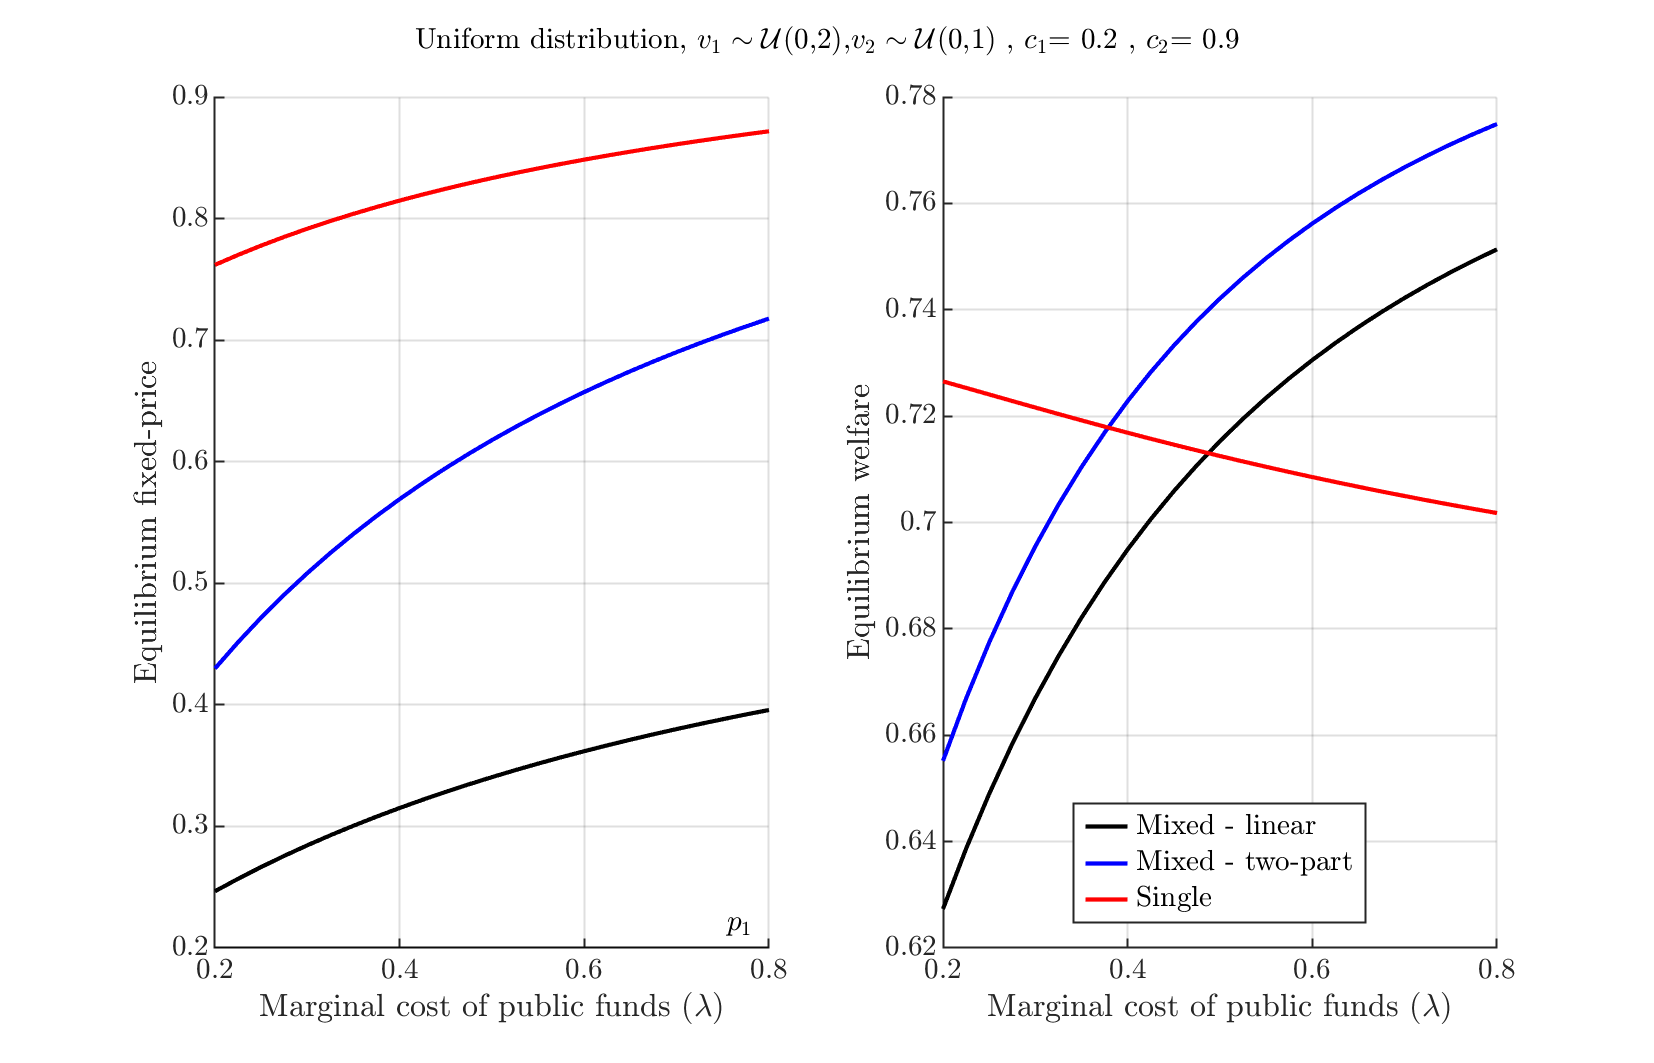
\includegraphics[width=0.9\linewidth]{figure/example_equ0_PublicFund_u.png}
        \caption{$W = CS + \Pi$.}
\end{figure}
    
\end{frame}



%%%%%%%%%%%%%%%%%%%%%%%%%%%%%%%%%%%%%%%%%%%%%%%%%%%%%%%%%%%%%%%%%%%%%%%%%%%%%%%%%%%%%%%%%%%%%%%%%%%%%%%%%%%%%%%%%%%%%%%%%%%%%%%%%%%%%%%%%%%%%%%%%%%%%%

\begin{frame}{Application - Consumer distribution}

\begin{figure}
    \centering
    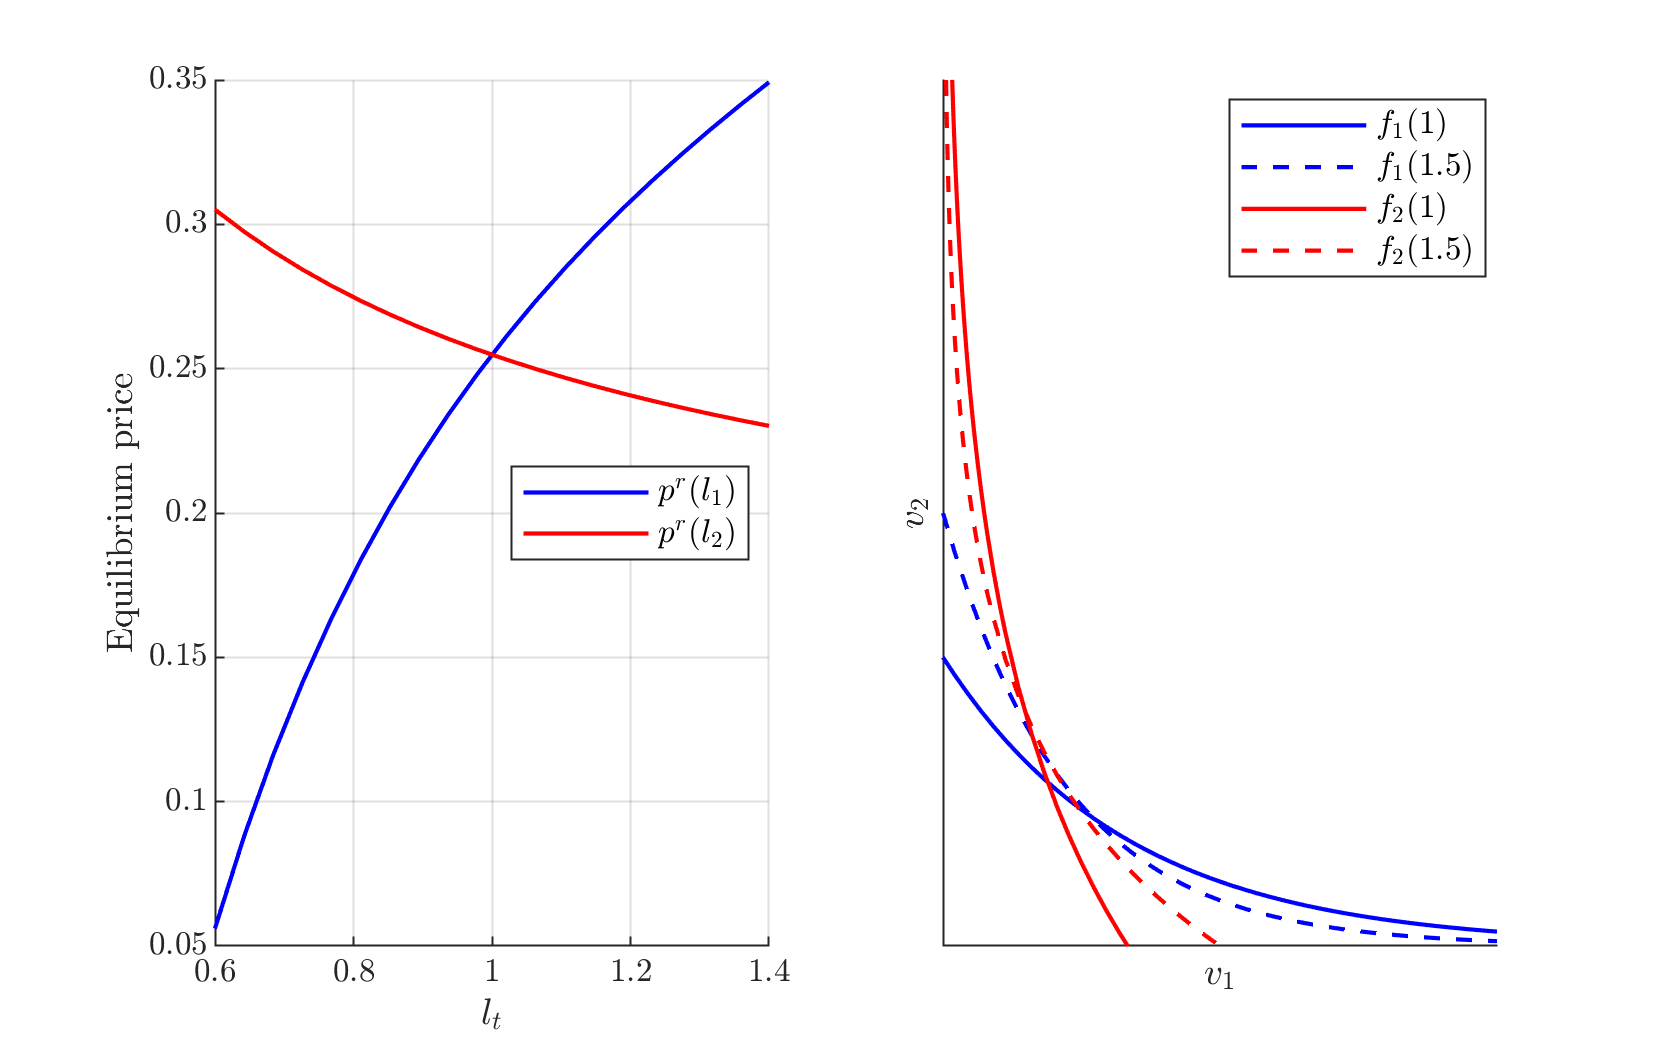
\includegraphics[width=0.95\linewidth]{figure/example_pdfeq.png}
    \caption{Exponential distribution: $v_t\sim \mathrm{Exp}(l_t)$ with $l_t>0$}
\end{figure}
    
\end{frame}



\section{Conclusion}



\begin{frame}{Conclusion}

\begin{itemize}
    \item The paper provides a novel framework describing the self-selection of electricity contracts by heterogeneous consumers.\vfill
    \item We show that the coexistence of a public option with a private sector and self-selection from consumers can lead to low welfare due to adverse selection. \vfill
    \item Going beyond the impossibility result: How to make the curves cross?  \vfill
    \begin{itemize}
        \item Different selection pattern: risk aversion. \vfill
        \item Barrier to selection: $p^r > AC(p^r)$. \vfill
        \item Lower retail cost: $\overline{AC}(p^r)<AC(p^r)$.
    \end{itemize}
    \vfill 
    \item Sophisticated firms: price discrimination $\approx$ public firm? 
\end{itemize}
    
\end{frame}

%%%%%%%%%%%%%%%%%%%%%%%%%%%%%%%%%%%%%%%%%%%%%%%%%%%%%%%%%%%%%%%%%%%%%%%%%%%%%%%%%%%%%%%%%%%%%%%%%%%%%%%%%%%%%%%%%%%%%%%%%%%%%%%%%%%%%%%%%%%%%%%%%%%%%%


\begin{frame}{}
  \centering {\Huge
  \emph{Thank you !}}
  
  \vspace{1cm}

  http://leopoldmonjoie.com/
\end{frame}
%%%%%%%%%%%%%%%%%%%%%%%%%%%%%%%%%%%%%%%%%%%%%%%%%%%%%%%%%%%%%%%%%%%%%%%%%%%%%%%%%%%%%%%%%%%%%%%%%%%%%%%%%%%%%%%%%%%%%%%%%%%%%%%%%%%%%%%%%%%%%%%%%%%%%%
%%%%%%%%%%%%%%%%%%%%%%%%%%%%%%%%%%%%%%%%%%%%%%%%%%%%%%%%%%%%%%%%%%%%%%%%%%%%%%%%%%%%%%%%%%%%%%%%%%%%%%%%%%%%%%%%%%%%%%%%%%%%%%%%%%%%%%%%%%%%%%%%%%%%%%
\bibliography{bib}



 \appendix


 
%%%%%%%%%%%%%%%%%%%%%%%%%%%%%%%%%%
%%%%%%%%%%%%%%%%%%%%%%%%%%%%%%%%%%%%%%%%%%%%%%%%%%%%%%%%%%%%%%%%%%%%%%%%%%%%%%%%%%%%%%%%%%%%%%%%%%%%%%%%%%%%%%%%%%%%%%%%%%%%%%%%%%%%%%%%%%%%%%%%%%%%%%




\begin{frame}{Illustration}\label{demand2}

\begin{figure}
    \centering
    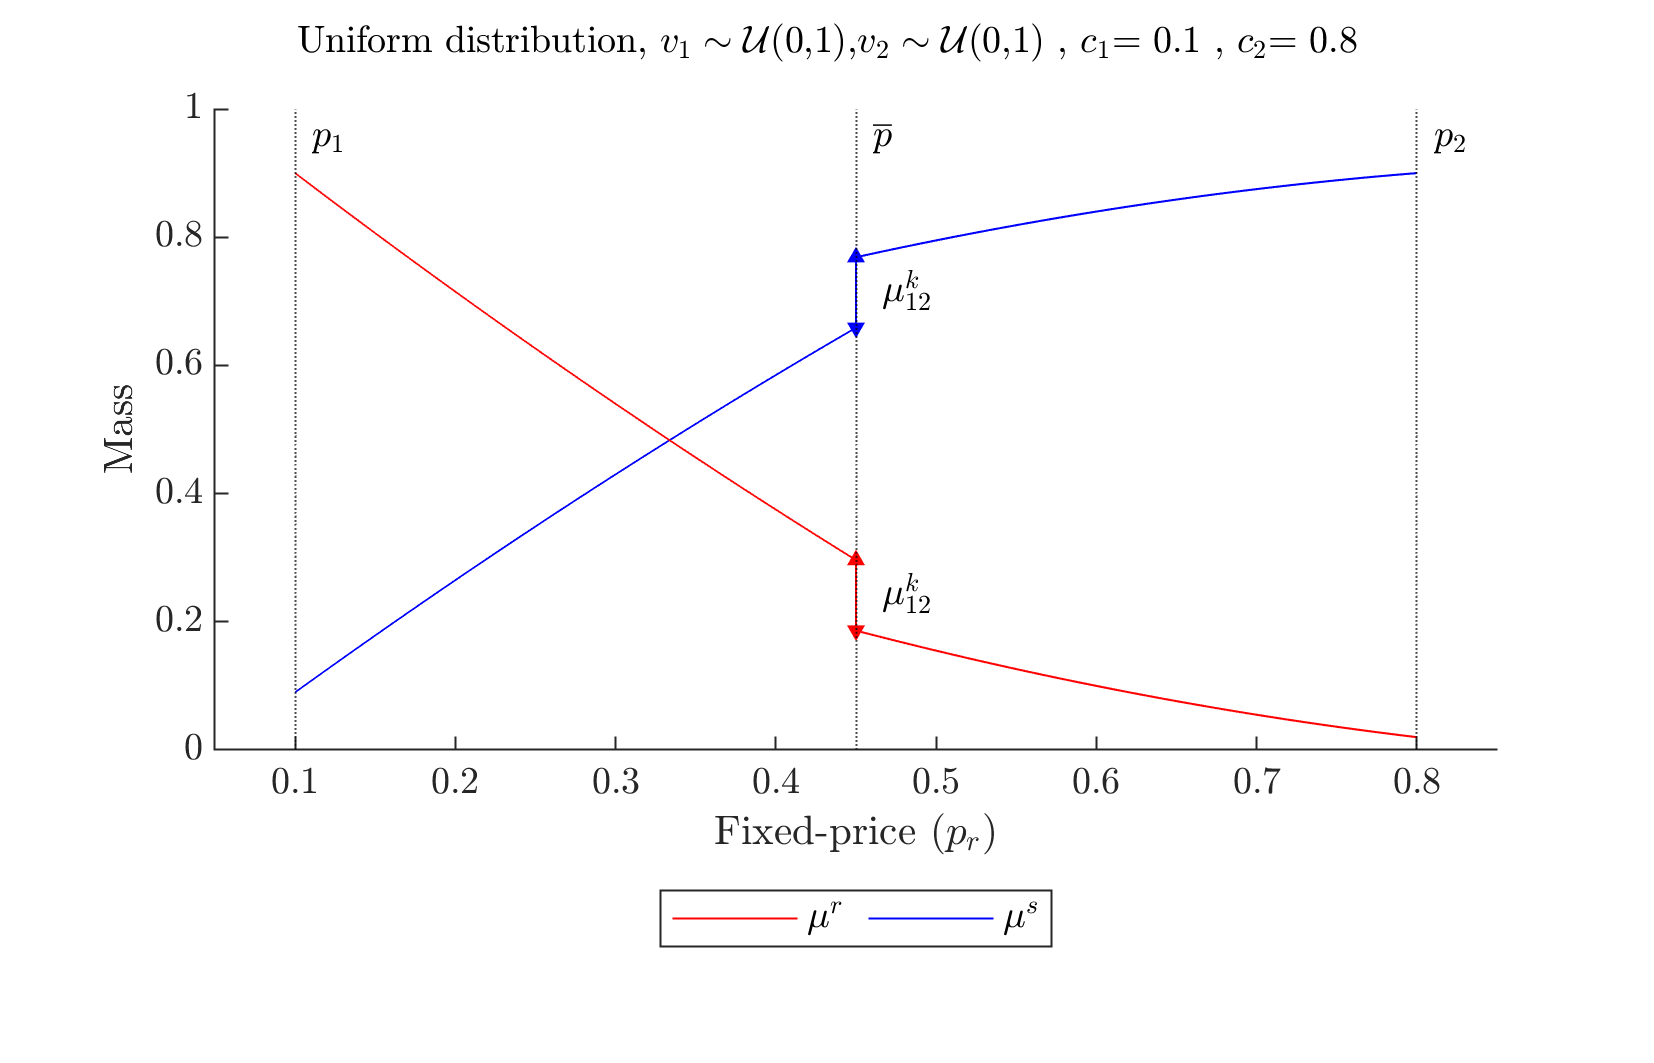
\includegraphics[width=1\linewidth]{figure/Demand_PR_unique.png}
    \caption{Demand is in line with the intuitions: decreasing for the FP and increasing for RTP.         \hyperlink{demand1}{\beamerreturnbutton{Go Back}}}
    \label{fig:Demand_PR}
    

\end{figure}
    
\end{frame}
%%%%%%%%%%%%%%%%%%%%%%%%%%%%%%%%%%%%%%%%%%%%%%%%%%%%%%%%%%%%%%%%%%%%%%%%%%%%%%%%%%%%%%%%%%%%%%%%%%%%%%%%%%%%%%%%%%%%%%%%%%%%%%%%%%%%%%%%%%
\begin{frame}{Example: Equilibrium benchmark with private firms}\label{EquilibriumSingle}

\begin{itemize}
    \item \boldrblue{First-best} - marginal cost pricing\vfill
    \[p_t = c_t\]  \vfill
    \item \boldrblue{Second-best} - weighted average marginal cost: \vfill
    \[p^\ast =     \sum_{t\in\{1,2\}} \omega^p_t c_t \quad \text{with} \quad \omega_t^p = \frac{\partial q_t^r / \partial p^r}{\partial q^r / \partial p^r} \quad  \text{and} \quad    \sum_{t\in\{1,2\}}  \omega_t^p =1 \] \vfill
    \item \boldrblue{Private firms FP} equilibrium - average cost \vfill
    \[ p^r = 
    AC^r(p^r)
    =
       \sum_{t\in\{1,2\}} \omega^{ac}_t c_t \quad \text{with} \quad \omega_t^{ac} = \frac{q_t^r(p^r)}{q^r(p^r)} \quad  \text{and} \quad    \sum_{t\in\{1,2\}}  \omega_t^{ac} =1 \] 
\end{itemize}


        \hyperlink{single}{\beamerreturnbutton{Go Back}}

\end{frame}

%%%%%%%%%%%%%%%%%%%%%%%%%%%%%%%%%%%%%%%%%%%%%%%%%%%%%%%%%%%%%%%%%%%%%%%%%%%%%%%%%%%%%%%%%%%%%%%%%%%%%%%%%%%%%%%%%%%%%%%%%%%%%%%%%%%%%%%%%%%%%%%%%%%%%%


\begin{frame}{Adverse selection in the single-contract case}\label{Adverse}

We define adverse (resp. advantageous) when for a given price $p^r$ 

\vfill

\[
AC^r(p^r) > MC^r(p^r) \quad (\text{resp.} <) 
\]

\vfill

The marginal consumer set is

\vfill

\[
    \mathcal{M}^r
    :=
    \left\{
    \mathbf{v}\in V:
    U(\mathbf{v},k)
    =
    \max\left\{0,\max_{\ell\neq k}U(\mathbf{v},\ell)\right\}
    \right\}.
\]

\vfill

Where $ MC^r(p^r)$ is the average cost of $\mathcal{M}^r$. 

\vfill

\[
    MC^r(p^r)
    =
    \sum_{t\in\{1,2\}}
    c_t  \cdot \frac{q^\mathcal{M}_t(p^r )
    }{q^\mathcal{M}(p^r )},  \qquad \text{where } \qquad q^\mathcal{M}_t = \int_{\mathcal{M}^r} x_t^*(\mathbf{v},k) f(\mathbf{v})\,d\mathbf{v}
\]


        \hyperlink{single}{\beamerreturnbutton{Go Back}}

\end{frame}

%%%%%%%%%%%%%%%%%%%%%%%%%%%%%%%%%%%%%%%%%%%%%%%%%%%%%%%%%%%%%%%%%%%%%%%%%%%%%%%%%%%%%%%%%%%%%%%%%%%%%%%%%%%%%%%%%%%%%%%%%%%%%%%%%%%%%%%%%%%%%%%%%%%%%%

\begin{frame}{Adverse selection in the single contract case}

\boldrblue{Semi-elasticity}: Define for an period $t$

\[ \sigma^{p}(q_t^r):= -\frac{\partial q_t^r}{\partial p^r}\frac{1}{q_t^r} \]

{\footnotesize
 $\approx$ density of marginal consumers in $t$ with respect to the density of inframarginal consumers
}

\vfill

\begin{proposition}\label{singleresult}
If private firms offer the FP contract, then 
\[p^r \ge p^\ast \quad  (\text{resp.} \le) \quad \text{iff} \quad  \sigma^{p}(q_1^r) \ge \sigma^{p}(q_2^r) \quad (\text{resp.} \le)\]

\end{proposition}

\vfill

\boldrblue{Note}: Similar results can be derived with the public firm on the sign of $A^r$.
            \hyperlink{single}{\beamerreturnbutton{Go Back}}

\end{frame}

%%%%%%%%%%%%%%%%%%%%%%%%%%%%%%%%%%
%%%%%%%%%%%%%%%%%%%%%%%%%%%%%%%%%%%%%%%%%%%%%%%%%%%%%%%%%%%%%%%%%%%%%%%%%%%%%%%%%%%%%%%%%%%%%%%%%%%%%%%%%%%%%%%%%%%%%%%%%%%%%%%%%%%%%%%%%%%%%%%%%%%%%%

\begin{frame}{Illustration}

\begin{figure}
    \centering
    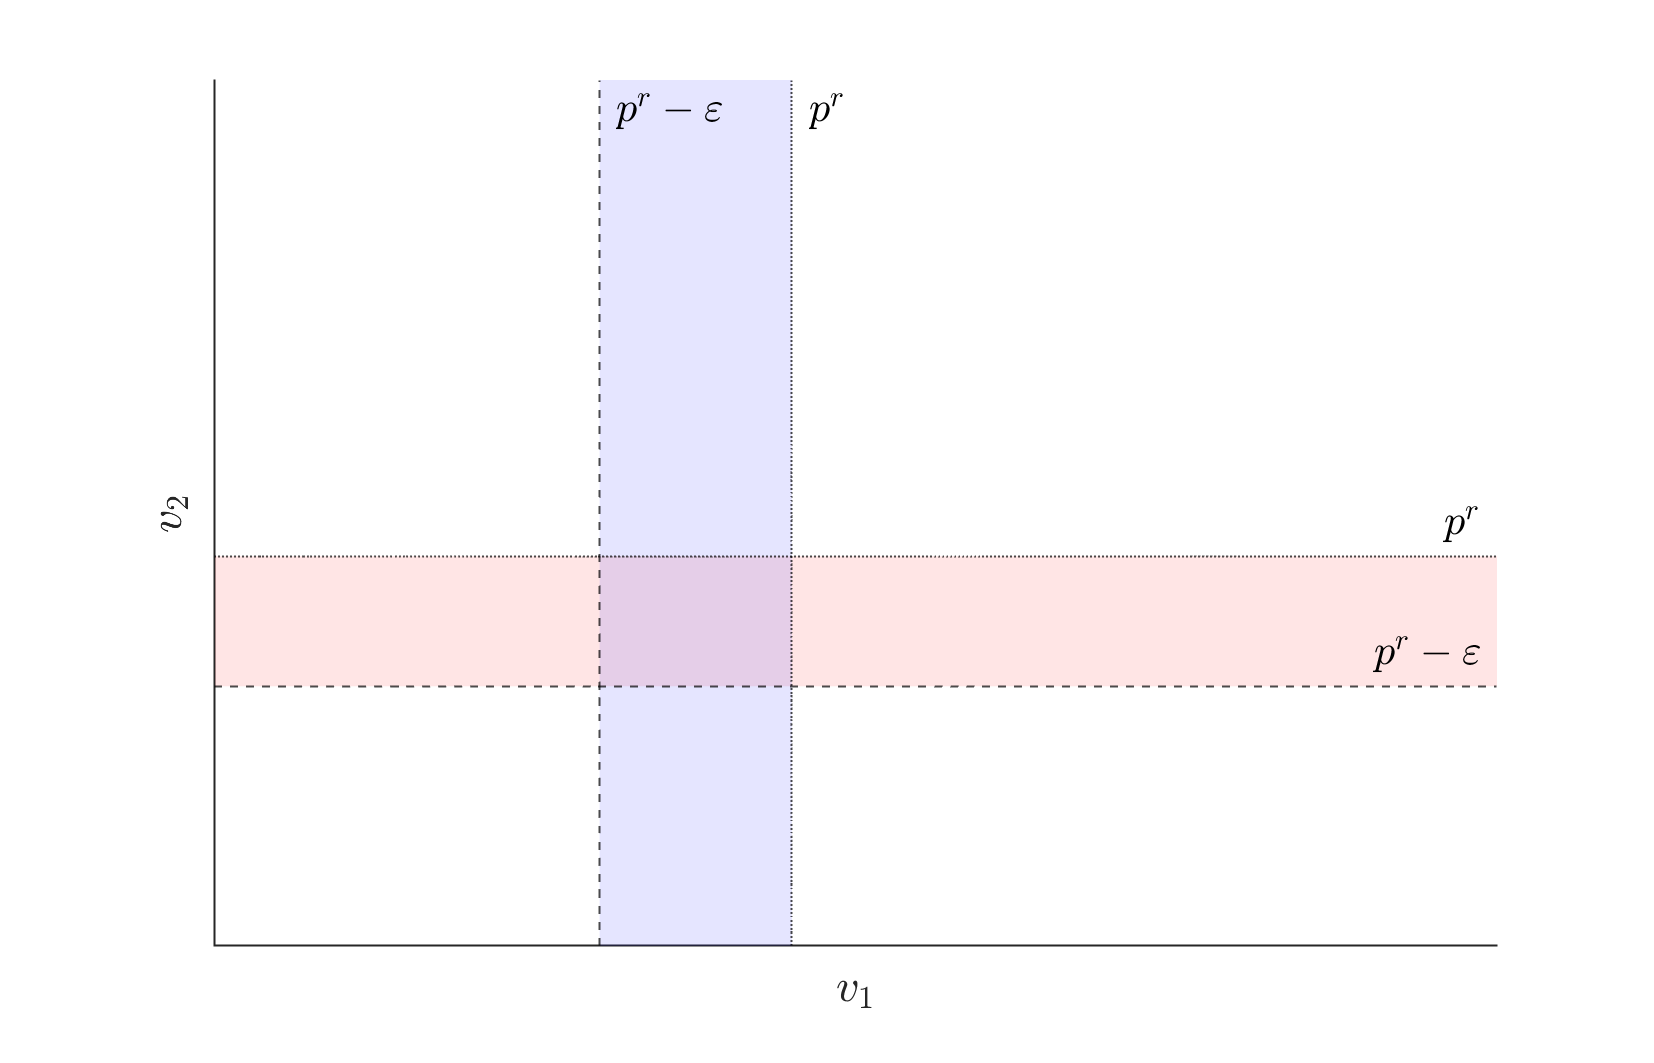
\includegraphics[width=0.8\linewidth]{figure/fp_demand_multi_deviation.png}
     \caption{Adverse/advantageous selection emerges when the share of marginal consumers differs across periods.         \hyperlink{single}{\beamerreturnbutton{Go Back}}} 
    \label{fig:fp_demand_multi_deviation}
\end{figure}
    
\end{frame}


%%%%%%%%%%%%%%%%%%%%%%%%%%%%%%%%%%%%%%%%%%%%%%%%%%%%%%%%%%%%%%%%%%%%%%%%%%%%%%%%%%%%%%%%%%%%%%%%%%%%%%%%%%%%%%%%%%%%%%%%%%%%%%%%%%%%%%%%%%%%%%%%%%%%%%
\begin{frame}{Extension Public Firm - Program         \hyperlink{ProgramMain}{\beamerreturnbutton{Go Back}}
}\label{ProgramExtension}

\begin{itemize}
    \item $\tau$ denotes a unit tax levied on all electricity consumption.  
\vfill
    \item The tax burden is split between the public firm's consumers and the rest of the market as follows:
\end{itemize}

\vfill

\[
\tau^r=\alpha \tau,\qquad \tau^s=(1-\alpha)\tau,\qquad \alpha\in[0,1].
\]

$\alpha=1$ corresponds to full self-financing

\vfill

\begin{definition}
A triple $(p^r,\tau,\textbf{p}^s)$ is a mixed-equilibrium contract with fiscal policy if, given consumers' optimal contract choice, $\pi^s(p^r,\tau,\textbf{p}^s)=0$ and $(p^r,\tau)$ solves
\begin{align*}\label{ObjFiscal}\tag{$\Omega^F$}
\max_{\{p^r,\tau\}} \quad & CS^r(p^r,\tau)\\
\text{s.t.}\quad
& \pi^r(p^r,\tau) \;+\; \tau^r q^r \;+\; \tau^s q^s \;=\;0,
\end{align*}
where $\pi^r(p^r,\tau)$ is the public firm's profit from serving its consumers at tariff $p^r$, and $\tau^r q^r+\tau^s q^s$ is the fiscal transfer financing the public firm.
\end{definition}


\end{frame}


\begin{frame}{Extension - Equilibrium \hyperlink{RamseyOutside}{\beamerreturnbutton{Go Back}}}\label{Ramseytax}
    
\begin{lemma}\label{lem:tax}
With a public firm and a full self-financing levy $\left(\alpha=1\right)$, there is no equilibrium with an active FP contract.
\end{lemma}

\begin{proposition}\label{prop:tax}
For $\alpha < 1$, there always exists an equilibrium $(p^r,\tau)$ such that some consumers strictly prefer the FP contract. The full price set by the firm solves the following:
 
\begin{equation*}
 P^r \;-\;
\underbrace{\sum_{t} c_t\,\frac{\delta_{\tau}(q_t^r)}{\delta_{\tau}(q^r)}}_{\text{marginal cost}} \;  = \; (1-\alpha)\underbrace{\Bigg. \frac{\lambda}{1+\lambda} \frac{q^r}{\delta_{\tau}(q^r)}\Bigg.}_{\text{Ramsey}}  \; - \;   \underbrace{\Bigg. \frac{1}{1+\lambda} \frac{\delta_\tau(\mathcal{C})}{\delta_\tau(q^r)} \Bigg.}_{\text{sorting correction}} \; - \;   \underbrace{ \Bigg. \frac{T}{\delta_{\tau}(q^r)}  \Bigg.}_{\text{levy effect}}  
\end{equation*}

where $T = q^s + t^s \delta_{\tau}(q^s)$

\end{proposition}

\end{frame}

 \end{document}


%%%%%%%%%%%%%%%%%%%%%%%%%%%%%%%%%%%%%%%%%%%%%%%%%%%%%%%%%%%%%%%%%%%%%%%%%%%%%%%%%%%%%%%%%%%%%%%%%%%%%%%%%%%%%%%%%%%%%%%%%%%%%%%%%%%%%%%%%%%%%%%%%%%%%%

\subsection{Extension - Ramsey and Taxation}

%%%%%%%%%%%%%%%%%%%%%%%%%%%%%%%%%%%%%%%%%%%%%%%%%%%%%%%%%%%%%%%%%%%%%%%%%%%%%%%%%%%%%%%%%%%%%%%%%%%%%%%%%%%%%%%%%%%%%%%%%%%%%%%%%%%%%%%%%%%%%%%%%%%%%%

\begin{frame}{Application with budget constraint }


\begin{itemize}
    \item We assume that the public firm relies on \boldrblue{two sources of financing}:  \vfill
    \begin{itemize}
        \item The profit from the regulated fixed-price contract.  \vfill
        \item Unitary tax $t$ levied on all electricity consumers. \vfill
    \end{itemize}
    \item $\alpha \in [0,1]$ is the tax share parameter, determining how the burden of supporting the public firm is shared between public and private consumers.  \vfill


\begin{equation*}
    \max_{p^r,t} CS^r(\textbf{p}_r,t) \hspace{0.5cm} \text{s.t.} \hspace{0.5cm}  \pi^r(\textbf{p}_r,t) + \alpha t q^r + (1-\alpha) t q_s = 0
\end{equation*}

\vfill

\item Full prices as $p^r = p^r + \alpha t$ and $P^s_t = p_t^s + (1-\alpha) t$

\end{itemize}

\end{frame}

%%%%%%%%%%%%%%%%%%%%%%%%%%%%%%%%%%%%%%%%%%%%%%%%%%%%%%%%%%%%%%%%%%%%%%%%%%%%%%%%%%%%%%%%%%%%%%%%%%%%%%%%%%%%%%%%%%%%%%%%%%%%%%%%%%%%%%%%%%%%%%%%%%%%%%

\begin{frame}{Intermediary results}

\begin{lemma}
For $\alpha = 1 $, there is no equilibrium with consumers having a strict preference for the fixed-price contract. 
\end{lemma}

\vfill

\begin{itemize}
    \item \boldrblue{A self-financing regulated firm} cannot offer a fixed-price contract in the equilibrium with self-selection.
    \vfill
    \begin{itemize}
    \item The result extends to individualized two-part tariff. 
    \end{itemize}
\end{itemize}

\vfill

\begin{lemma}

\vspace{0.1cm}

For $\alpha \in [0,1)$, the equilibrium full prices are independent of $\alpha$ 

\end{lemma}

\vfill

\begin{itemize}
    \item The regulated firm chooses $p^r$ and $t$ such that the demand for contracts remains the same for any $\alpha$. The new decision variables are $p^r$ and $t_s=(1-\alpha)t$
\end{itemize}
    
\end{frame}

%%%%%%%%%%%%%%%%%%%%%%%%%%%%%%%%%%%%%%%%%%%%%%%%%%%%%%%%%%%%%%%%%%%%%%%%%%%%%%%%%%%%%%%%%%%%%%%%%%%%%%%%%%%%%%%%%%%%%%%%%%%%%%%%%%%%%%%%%%%%%%%%%%%%%%


\begin{frame}{Public firm equilibrium}

\begin{proposition}

\vspace{0.1cm}

For $\alpha < 1$, there always exist $(p^r,t)$ such that some consumers strictly prefer the FP contract. The full price sets by the firm solves the following:
 
\begin{equation*}
 p^r \;  = \; \underbrace{\Bigg.\frac{(1-\alpha)\lambda}{1+\lambda} \frac{q^r}{\delta^{t_s}(q^r)}\Bigg.}_{\text{Ramsey}} \; +\;   \underbrace{    \sum_{t\in\{1,2\}} \textcolor{red}{p_t^w }\textcolor{blue}{\frac{\delta^{t_s}(q^r_t)}{\delta^{t_s}(q^r)}}}_{\text{marg. cost}}    \; - \;   \underbrace{\Bigg. \frac{1}{1+\lambda} \frac{W(\mathcal{M}^s)}{\delta^{t_s}(q^r)} \Bigg.}_{\text{foregone surplus}} \; - \;   \underbrace{ \Bigg. \frac{T}{\delta^{t_s}(q^r)}  \Bigg.}_{\text{levy effect}}  
\end{equation*}

With $\delta^{t_s}(q) = \partial_{t_s} q-\partial_p q$ and $W(\mathcal{M}^s)>0$
\end{proposition}

\vfill

\begin{itemize}
    \item  $T$ = marginal revenue of the tax from the private consumers.

\begin{equation*}
        T = q^s + t_s \delta^{t_s}(q^s)
\end{equation*}

\end{itemize}



\end{frame}

%%%%%%%%%%%%%%%%%%%%%%%%%%%%%%%%%%%%%%%%%%%%%%%%%%%%%%%%%%%%%%%%%%%%%%%%%%%%%%%%%%%%%%%%%%%%%%%%%%%%%%%%%%%%%%%%%%%%%%%%%%%%%%%%%%%%%%%%%%%%%%%%%%%%%%

\begin{frame}{Illustration}

\begin{figure}
    \centering
    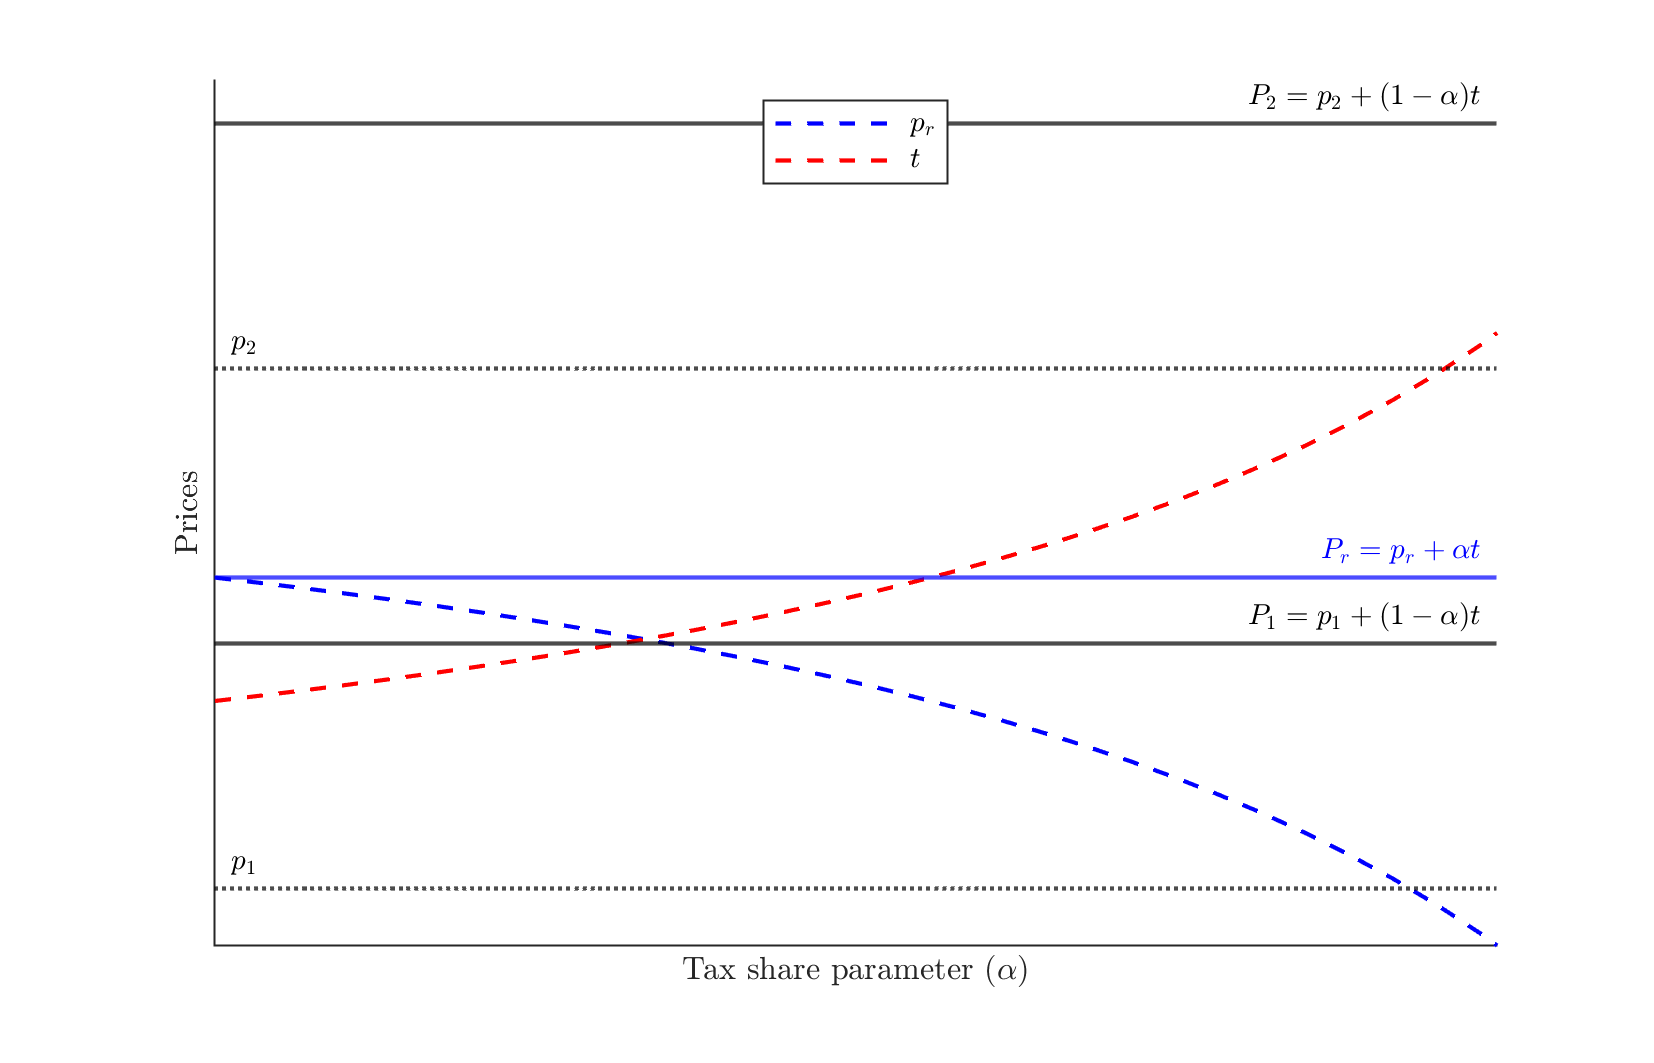
\includegraphics[width=1\linewidth]{figure/Indep_alpha_tax.png}
    \caption{The equilibrium full prices for the private and public consumers are independent of the tax share parameter $\alpha$.}
    \label{fig:Indep_alpha_tax}
\end{figure}
    
\end{frame}

%%%%%%%%%%%%%%%%%%%%%%%%%%%%%%%%%%%%%%%%%%%%%%%%%%%%%%%%%%%%%%%%%%%%%%%%%%%%%%%%%%%%%%%%%%%%%%%%%%%%%%%%%%%%%%%%%%%%%%%%%%%%%%%%%%%%%%%%%%%%%%%%%%%%%%

\subsection{Extension - Two-part tariff}

\begin{frame}{Public firm equilibrium with a two part tariff}


\begin{proposition}

Starting from $p^r = p_2$, the public firm has an incentive to introduce a fixed-price contract if the following condition holds:

\[ CS(\mathcal{M}^s) > \lambda q^r_2(p_2) \]

\end{proposition}

\begin{itemize}
    \item A two-part tariff does not change the incentives to offer a fixed-price contract. 
\end{itemize}

\begin{proposition}
 
The two-part tariff of the fixed-price contract with the public firm solves the following modified Ramsey prices:
 
\begin{equation*}
      p^r = \underbrace{\bigg.\frac{\lambda}{1+\lambda}\frac{q^r}{ \textcolor{blue}{\delta^A(q^r)}}\left(1 - \frac{\mu_r}{q^r}\right)+     \sum_{t\in\{1,2\}} \textcolor{red}{p_t^w }\textcolor{blue}{\frac{\delta^A(q^r_t)}{\delta^A(q^r)}} - A \textcolor{blue}{\frac{\delta^A\mu}{\delta^A(q^r)}} \bigg.}_{\text{similar term as in the single contract case}} -  \;   \underbrace{\bigg. \frac{1}{1+\lambda} \frac{W(\mathcal{M}^s)}{\delta^A(q^r)} \bigg.}_{\text{foregone surplus}}
\end{equation*}

\end{proposition}
    
\end{frame}


\appendix

%%%%%%%%%%%%%%%%%%%%%%%%%%%%%%%%%%%%%%%%%%%%%%%%%%%%%%%%%%%%%%%%%%%%%%%%%%%%%%%%%%%%%%%%%%%%%%%%%%%%%%%%%%%%%%%%%%%%%%%%%%%%%%%%%%%%%%%%%%%%%%%%%%%%%%

\begin{frame}{Literature: Contracts in electricity market}\label{Lit_FB}

\begin{itemize}
    \item Peak Load Pricing Theory: Optimal investment in electricity markets requires short-term marginal cost pricing \cite{m1949tarification,joskow2007reliability}. \vfill

\item Contracts that approximate the first-best.
    \begin{itemize}
        \item  TOU and CPP / Demand Response / RTP \cite{Hinchberger2024}
    \end{itemize}

    \vfill

\item Real-time pricing (RTP)
    \begin{itemize}
        \item Seminal modeling papers comparing fixed-price contracts and RTP contracts with short-term and long-term interactions: \cite{Borenstein2003,Borenstein2005a,Borenstein2005b}
        \item Reduction of market power: \cite{Poletti2020}
        \item Reduction of pollution: \cite{Borenstein2021} 
        \item Interaction with renewable technology: \cite{Imelda2024}
        \item Interaction with decarbonization technologies: \cite{bailey2024electric}
    \end{itemize}
\end{itemize}

    \vfill
    
 \hyperlink{Motivations}{\beamergotobutton{Back}}
    
\end{frame}



%%%%%%%%%%%%%%%%%%%%%%%%%%%%%%%%%%%%%%%%%%%%%%%%%%%%%%%%%%%%%%%%%%%%%%%%%%%%%%%%%%%%%%%%%%%%%%%%%%%%%%%%%%%%%%%%%%%%%%%%%%%%%%%%%%%%%%%%%%%%%%%%%%%%%%



%%%%%%%%%%%%%%%%%%%%%%%%%%%%%%%%%%%%%%%%%%%%%%%%%%%%%%%%%%%%%%%%%%%%%%%%%%%%%%%%%%%%%%%%%%%%%%%%%%%%%%%%%%%%%%%%%%%%%%%%%%%%%%%%%%%%%%%%%%%%%%%%%%%%%%

\begin{frame}{Available technology and contract options}\label{options1}

\begin{columns}

\begin{column}{0.55\textwidth}  %%<--- here
    \begin{center}
\begin{figure}
    \centering
    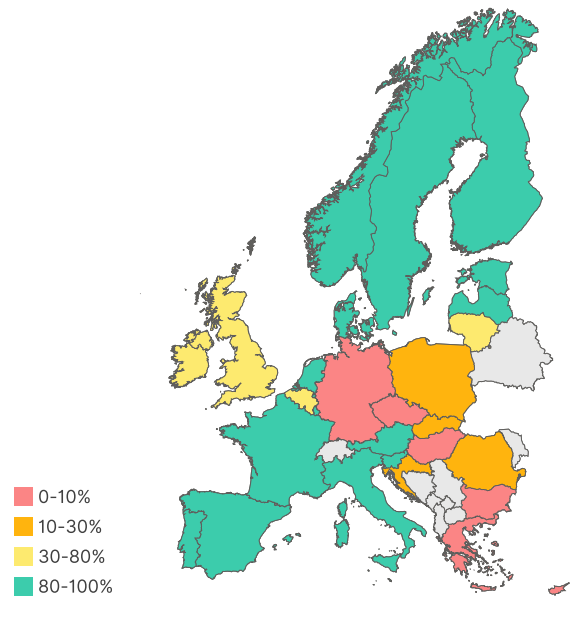
\includegraphics[width=0.75\linewidth]{figure/Smart_EU.PNG}
    \caption{Roll-out of smart meters among households \cite{ACER2024} }
    \label{fig:Smart_EU}
\end{figure}
     \end{center}
\end{column}
\begin{column}{0.50\textwidth}
\small	
 \boldrblue{20 EU countries out of 29} have regulated and non-regulated dynamic contract options for households \cite{ACER2024}
\hyperlink{ContractType}{\beamergotobutton{Table}},\hyperlink{USdata}{\beamergotobutton{US Data}},\hyperlink{options2}{\beamergotobutton{Details}},\hyperlink{UptakeContract1}{\beamergotobutton{Back 1}},\hyperlink{UptakeContract2}{\beamergotobutton{Back 2}}
\hspace{2cm}
\end{column}
\end{columns}

\end{frame}


%%%%%%%%%%%%%%%%%%%%%%%%%%%%%%%%%%%%%%%%%%%%%%%%%%%%%%%%%%%%%%%%%%%%%%%%%%%%%%%%%%%%%%%%%%%%%%%%%%%%%%%%%%%%%%%%%%%%%%%%%%%%%%%%%%%%%%%%%%%%%%%%%%%%%%

\begin{frame}{Available technology and contract options}\label{options2}

% \begin{columns}

% \begin{column}{0.55\textwidth}  %%<--- here
%     \begin{center}
% \begin{figure}
%     \centering
%     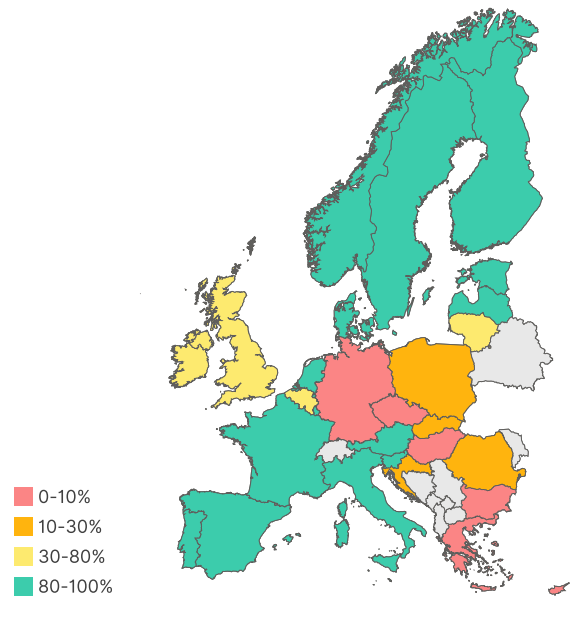
\includegraphics[width=0.75\linewidth]{figure/Smart_EU.PNG}
%     \caption{Roll-out of smart meters among households \cite{ACER2024} }
%     \label{fig:Smart_EU}
% \end{figure}
%      \end{center}
% \end{column}
% \begin{column}{0.50\textwidth}
% \small	
%  \boldrblue{20 EU countries out of 29} have regulated and non-regulated dynamic contract options for households \cite{ACER2024}

% \hspace{2cm}

\begin{figure}
    \centering
    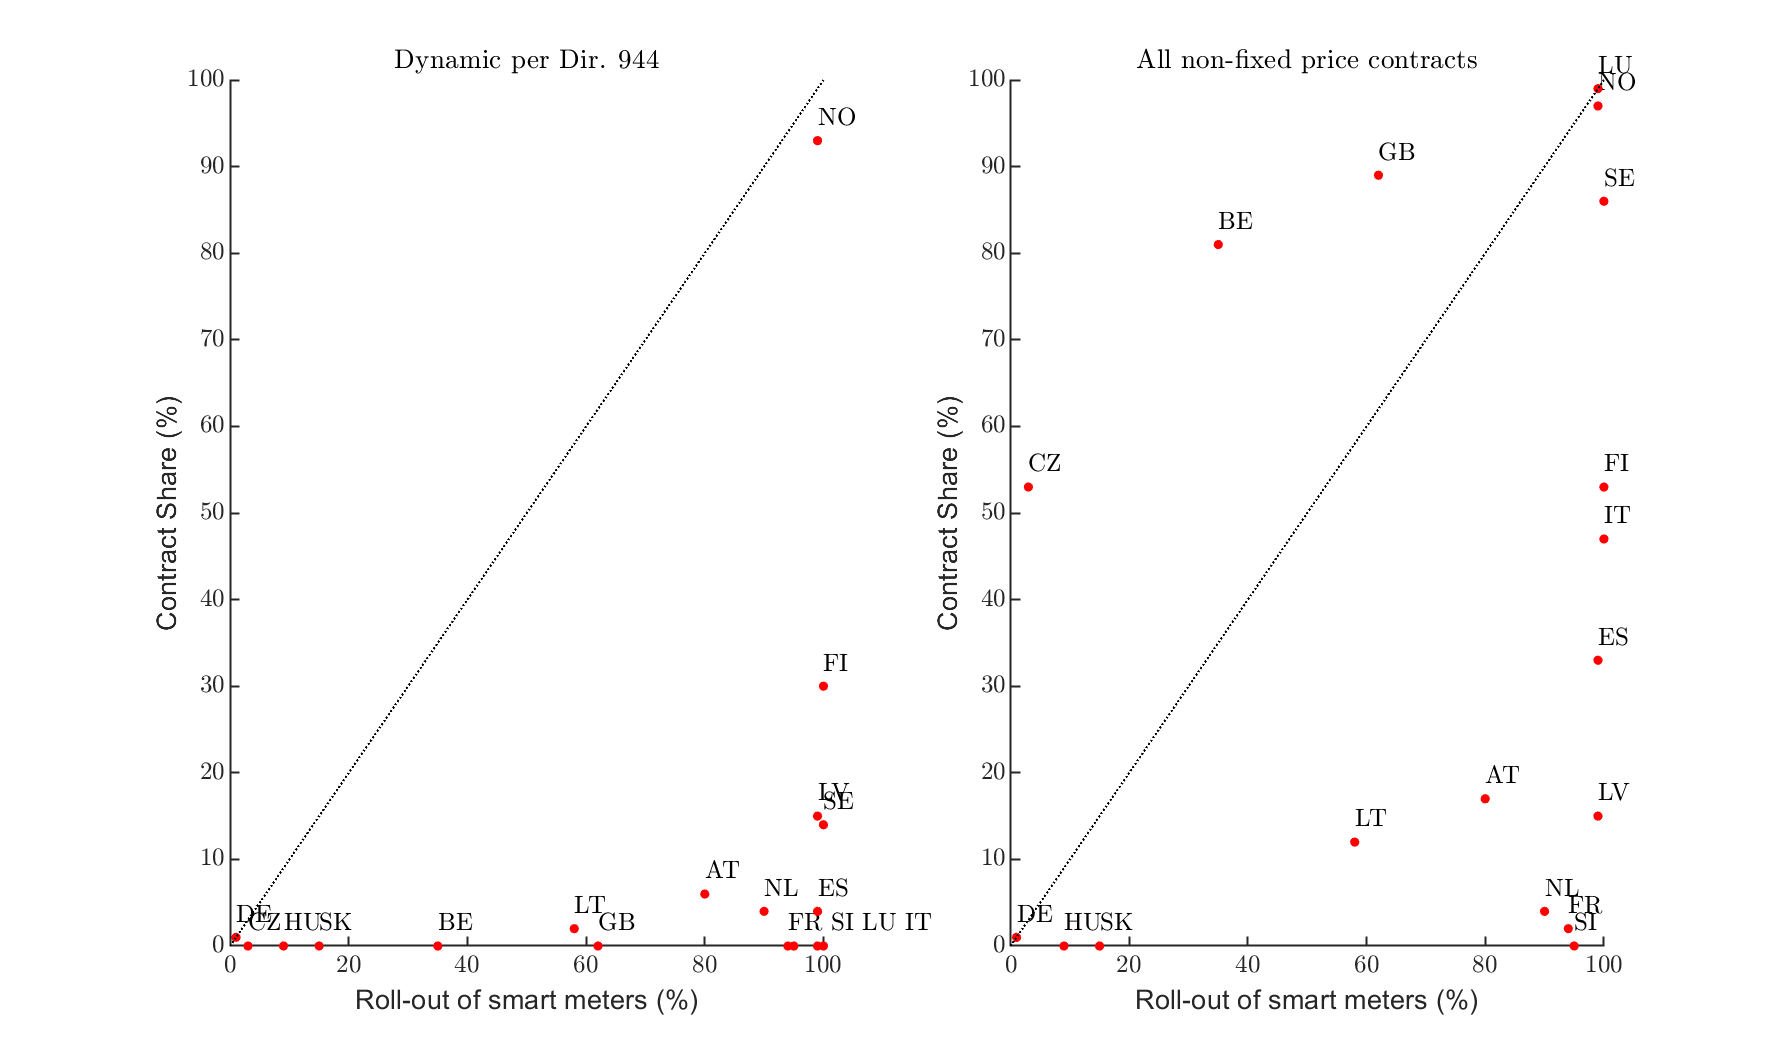
\includegraphics[width=1\linewidth]{figure/share_contract.PNG}
    \caption{Share of contract uptakes with respect to share of roll-out of smart meters among households (own calculation based on \cite{ACER2024}),\hyperlink{ContractType}{\beamergotobutton{Table}},\hyperlink{USdata}{\beamergotobutton{US Data}},\hyperlink{options1}{\beamergotobutton{Back}}}
    \label{fig:share_contract}
\end{figure}







% \end{column}
% \end{columns}



\end{frame}


%%%%%%%%%%%%%%%%%%%%%%%%%%
%%%%%%%%%%%%%%%%%%%%%%%%%%%%%%%%%%%%%%%%%%%%%%%%%%%%%%%%%%%%%%%%%%%%%%%%%%%%%%%%%%%%%%%%%%%%%%%%%%%%%%%%%%%%%%%%%%%%%%%%%%%%%%%%%%%%%%%%%%%%%%%%%%%%%%

\begin{frame}{Contract Options in the EU}\label{ContractType}

\begin{figure}
    \centering
    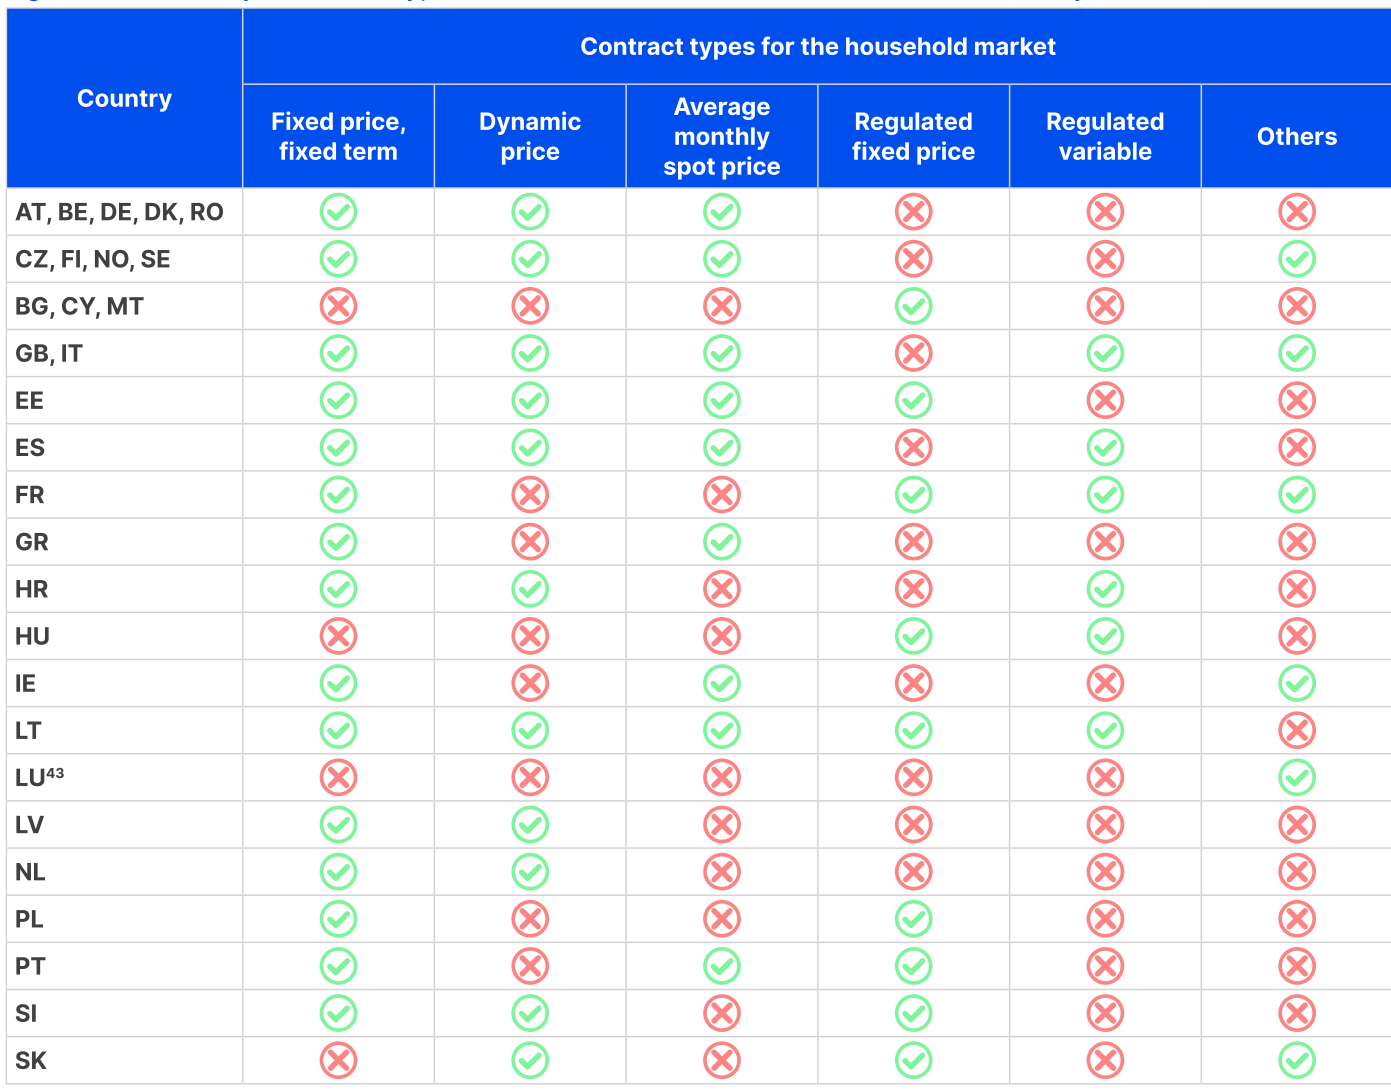
\includegraphics[width=0.8\linewidth]{figure/ContractType.PNG}
    \caption{Availability of different types of contracts to customers in the household electricity market in 2023 Country.\cite{ACER2024}  \hyperlink{options1}{\beamergotobutton{Back}} }
    \label{fig:ContractType}
\end{figure}
    
\end{frame}



%%%%%%%%%%%%%%%%%%%%%%%%%%%%%%%%%%%%%%%%%%%%%%%%%%%%%%%%%%%%%%%%%%%%%%%%%%%%%%%%%%%%%%%%%%%%%%%%%%%%%%%%%%%%%%%%%%%%%%%%%%%%%%%%%%%%%%%%%%%%%%%%%%%%%%

\begin{frame}{US Data}\label{USdata}

\begin{figure}
    \centering
    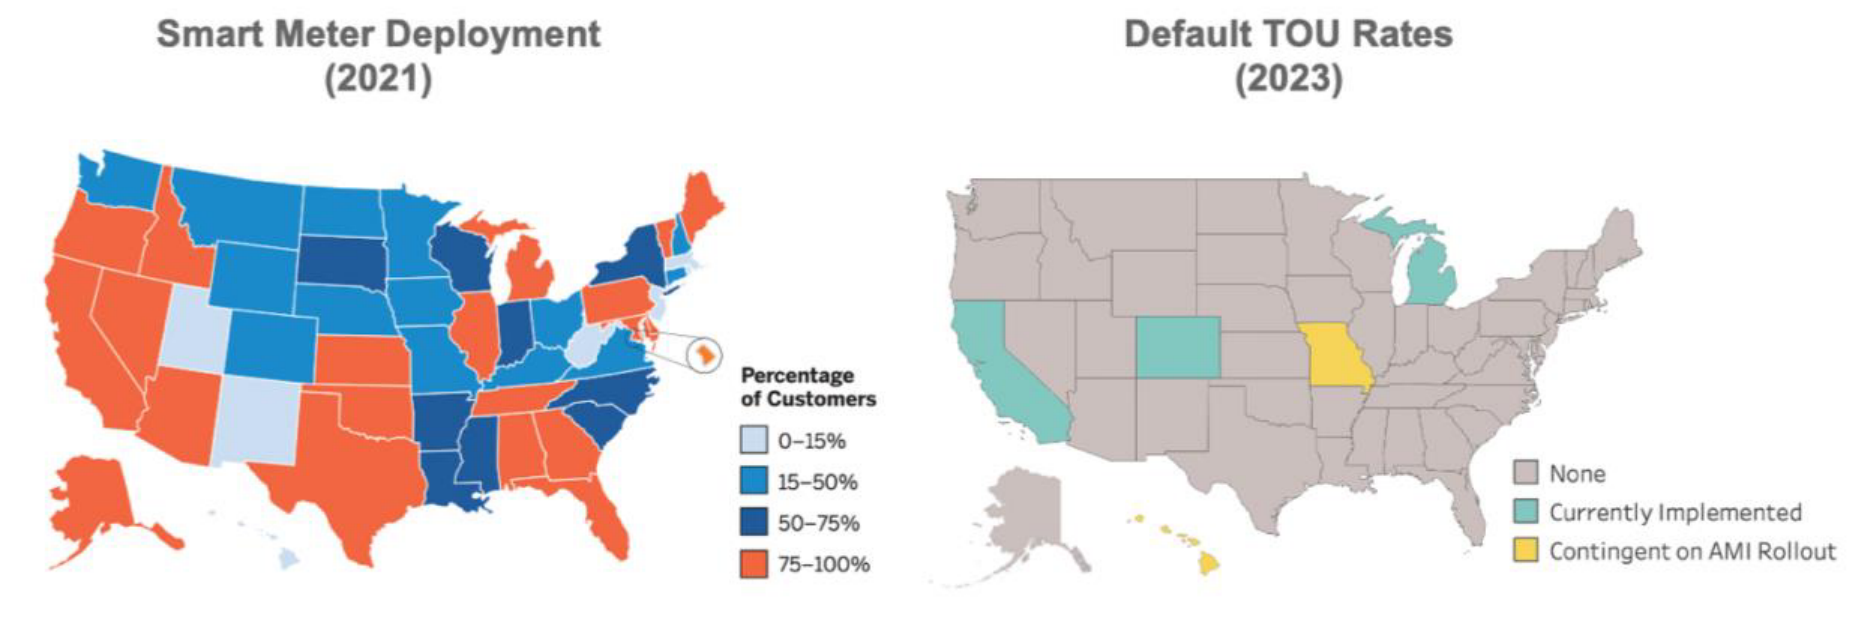
\includegraphics[width=1\linewidth]{figure/FP_Smart_US.PNG}
    \caption{Smart meter deployment among US households (left) and default TOU rate adoption (right). Default TOU rates are shown for each state's largest distribution utility. \cite{Turk2024}  \hyperlink{options1}{\beamergotobutton{Back}} }
    \label{fig:FP_Smart_US}
\end{figure}
    
\end{frame}

%%%%%%%%%%%%%%%%%%%%%%%%%%%%%%%%%%%%%%%%%%%%%%%%%%%%%%%%%%%%%%%%%%%%%%%%%%%%%%%%%%%%%%%%%%%%%%%%%%%%%%%%%%%%%%%%%%%%%%%%%%%%%%%%%%%%%%%%%%%%%%%%%%%%%%

\begin{frame}{Example - Adverse selection}\label{AdverseSelectionSingle_graph}
    \begin{figure}
        \centering
        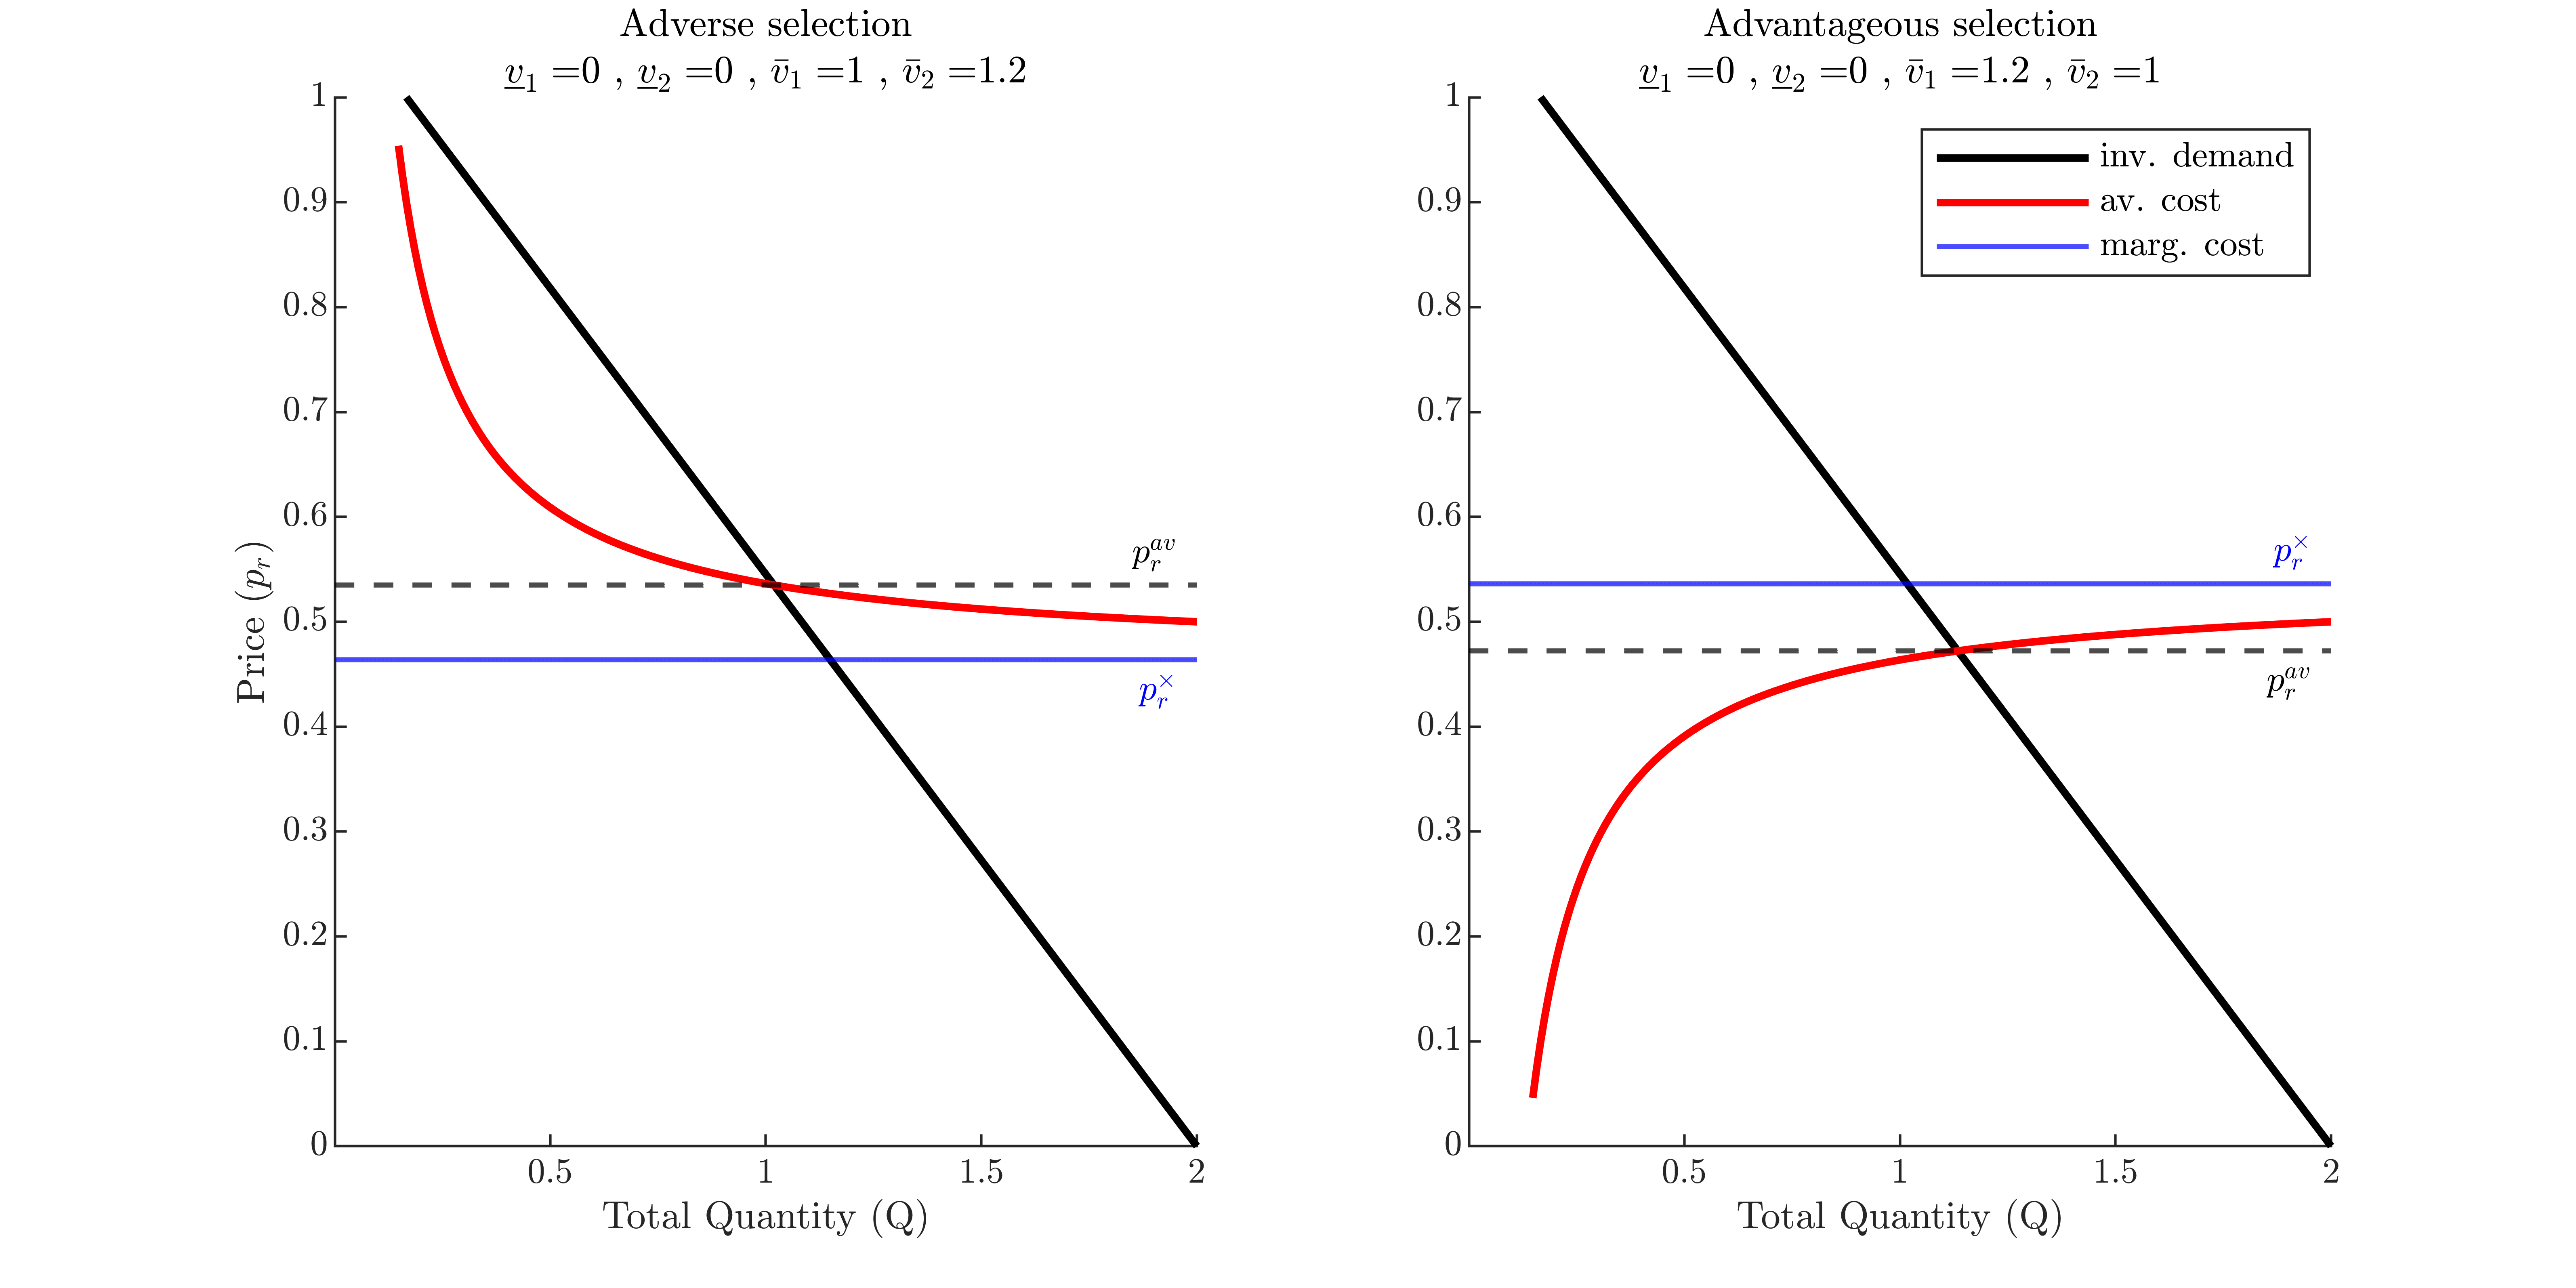
\includegraphics[width=1\linewidth]{figure/Exemple_AS_u_ddeAC.png}
        \caption{Illustration with uniform distribution distribution. $\sigma_t = \frac{1}{\bar{v}_t - p^r} $ \hyperlink{AdverseSelectionSingle}{\beamergotobutton{Back}}}
    \end{figure}
\end{frame}

%%%%%%%%%%%%%%%%%%%%%%%%%%%%%%%%%%%%%%%%%%%%%%%%%%%%%%%%%%%%%%%%%%%%%%%%%%%%%%%%%%%%%%%%%%%%%%%%%%%%%%%%%%%%%%%%%%%%%%%%%%%%%%%%%%%%%%%%%%%%%%%%%%%%%%

\begin{frame}{Proof - Adverse Selection Private Firms}\label{AdverseSelectionSingle_proof}


\begin{equation*}
    C^r(p^r) = \int_{S^r} c(\textbf{v}) f(\textbf{v}) d\textbf{v} = \sum_{t=\{1,2\}}q_t^r p_t^w
\end{equation*}

Which implies the average cost

\begin{equation*}
    AC^r(p^r) =  \mathbb{E}[c(\textbf{v})|\mathcal{S}^r] =   \frac{1}{q^r}C^k = \frac{1}{q^r}(q_1^r p_1^w + q_2^r p_2^w)
\end{equation*}

The derivative of the average cost is:

\begin{equation*}
    \frac{\partial AC^r(p^r)}{\partial p^r} = \frac{q_1^rq_2^r}{q^r_2} (p_2^w - p_1^w)\left( \frac{\partial q_2^r}{\partial p^r} \frac{1}{q_2^r} -\frac{\partial q_1^r}{\partial p^r} \frac{1}{q_1^r}\right)
\end{equation*}

Hence:

\begin{equation*}
    \frac{\partial AC^r(p^r)}{\partial p^r} = \frac{q_1^rq_2^r}{q^r_2} (p_2^w - p_1^w)\left( \sigma_1^r -\sigma_2^r\right)
\end{equation*}

\hyperlink{AdverseSelectionSingle}{\beamergotobutton{Back}}


\end{frame}

%%%%%%%%%%%%%%%%%%%%%%%%%%%%%%%%%%%%%%%%%%%%%%%%%%%%%%%%%%%%%%%%%%%%%%%%%%%%%%%%%%%%%%%%%%%%%%%%%%%%%%%%%%%%%%%%%%%%%%%%%%%%%%%%%%%%%%%%%%%%%%%%%%%%%%

\begin{frame}{Proof - Two-part Tariff Public Firm}\label{ProfitTPTSingle_proof}


\begin{equation*}
    \frac{\partial O^r}{\partial A}(p^r,A) = \lambda \mu_r + (1 + \lambda)\left( (p^r - p_1^w) \frac{\partial q_1^r}{\partial  A} + (p^r - p_1^w) \frac{\partial q_2^r}{\partial  A} + A \frac{\partial \mu_r}{\partial  A}\right) 
\end{equation*}

Using 

\[ p^r^\times = p_1^w\frac{\partial q_1^r/ \partial p^r}{\partial q^r/ \partial p^r} + p_2^w \frac{\partial q_2^r/ \partial p^r}{\partial q^r/ \partial p^r}\]

we have $ \frac{\partial O^r}{\partial A}(p^r^\times,0)  > 0$ if and only if:

\begin{equation*}
    \frac{\lambda}{1+\lambda}\mu_r + (p_2^w - p_1^w)\frac{q^e_1 q^e_2}{q^e}\left( \frac{\sigma_1^i}{\sigma_1^e} - \frac{\sigma_2^i}{\sigma_2^e} \right) > 0 
\end{equation*}


\hyperlink{ProfitTPTSingle}{\beamergotobutton{Back}}


\end{frame}



\end{document}


%%%%%%%%%%%%%%%%%%%%%%%%%%%%%%%%%%%%%%%%%%%%%%%%%%%%%%%%%%%%%%%%%%%%%%%%%%%%%%%%%%%%%%%%%%%%%%%%%%%%%%%%%%%%%%%%%%%%%%%%%%%%%%%%%%%%%%%%%%%%%%%%%%%%%%

% \begin{frame}{With the public firm }\label{RamseyMonopoly}


% \begin{itemize}
%     \item We assume that the public firm relies on two sources of financing:  \vfill
%     \begin{itemize}
%         \item The profit from the regulated fixed-price contract.  \vfill
%         \item Unitary tax $t$ levied on all electricity consumers. \vfill
%     \end{itemize}
% \end{itemize}

% \begin{result}

% \vspace{0.1cm}

% There exist some consumers who strictly prefer the FP contract. The full price ($p^r+t_r$) set by the firm solves the following:
 
% \begin{equation*}
%  p^r^{**} \; = p^r^{**} +t_r^{**} \;  = \;  \text{av.marg.cost} \; + \; \text{ramsey}  \; - \;   \underbrace{\bigg. \Omega \bigg.}_{\text{foregone CS}} \; - \;   \underbrace{ \bigg. T \bigg.}_{\text{levy effect}}  
% \end{equation*}

% \end{result}

% \begin{itemize}
%     \item  $T$ = marginal revenue of the tax from the private consumers
%     \item  $\Omega$ = welfare of the \textit{contract switchers}
% \end{itemize}




% \end{frame}







\newcounter{totalbeforeappendix}
\setcounter{totalbeforeappendix}{\value{framenumber}}
\addtocounter{totalbeforeappendix}{2} 
\addtocounter{framenumber}{-9}


\begin{frame}{Literature: Demand for contracts}\label{Lit_Conso}

\begin{itemize}
    \item \textbf{No theoretical foundation of self-selection in the power retail market}.

    \vfill
    
    \item Variation of an \boldrblue{exogenous share} of RTP consumers.
    \begin{itemize}
        \item Seminal paper: \cite{Borenstein2005b}, Technological cost \cite{Leautier2014},  Interactions with renewable technologies \cite{Ambec2021}, Risk aversion \cite{Boom2021}.
        \item \boldrblue{limits}: single period - homogenous consumers. 
    \end{itemize}

 \vfill

    \item \boldrblue{Empirical evidence} of self-selection with heterogeneous consumers
    \begin{itemize}
        \item Adverse selection \cite{Ito2023} Risk aversion \cite{Qiu2018} Behavioral bias \cite{Hortacsu2017,Fowlie2021}
        \item \boldrblue{limits}: focus on behavioral biais.
    \end{itemize}


\vfill
    \item Empirical evidence of RTP contracts.
    
    \begin{itemize}
        \item Effect of contract prices on consumption \cite{Fabra2021,Han2023,Enrich2024,Fu2024}, Redistributive effect \cite{Leslie2021, Levinson2022a, Cahana2023}
    \end{itemize}


     
    
\end{itemize}

\vfill

\hyperlink{FirstCont}{\beamergotobutton{Back}}

\end{frame}

%%%%%%%%%%%%%%%%%%%%%%%%%%%%%%%%%%%%%%%%%%%%%%%%%%%%%%%%%%%%%%%%%%%%%%%%%%%%%%%%%%%%%%%%%%%%%%%%%%%%%%%%%%%%%%%%%%%%%%%%%%%%%%%%%%%%%%%%%%%%%%%%%%%%%%

\begin{frame}{Literature: Retail competition}\label{Lit_Mkt1}
    
    
\begin{itemize}
    \item \textbf{Little attention on the competition in the retail market and contract equilibrium}.  
    
    \vfill

    \item Few empirical works on the benefit of retail competition \cite{Concettini2013}. Retailers acting as in Bertrand competition \cite{von2010electricity}
    
    \vfill

   \item Seminal papers \cite{joskow2006retail} and \cite{Borenstein2003}. \boldrblue{limits}: homogeneous consumers - simplified market structure.

\vfill

   \item  \boldrblue{Adverse selection} in retail electricity market
   
   \begin{itemize}
       \item Consumers deviation \cite{chao2013incentive}
       \item IC contracts and market equilibrium \cite{Astier2021}
   \end{itemize}

\vfill

    \item \boldrblue{Outside public option with incomplete information}
    \begin{itemize}
        \item In electricity markets with a regulated firm with redistributive preferences \cite{Martimort2020a} in a general setting \cite{Kang2023a}
    \end{itemize}


% \vfill

% \item Market power and price discrimination in retail electricity market \cite{byrne2022price}

\end{itemize}

\vfill



\hyperlink{SecondCont}{\beamergotobutton{Back}}

\end{frame}


%%%%%%%%%%%%%%%%%%%%%%%%%%%%%%%%%%%%%%%%%%%%%%%%%%%%%%%%%%%%%%%%%%%%%%%%%%%%%%%%%%%%%%%%%%%%%%%%%%%%%%%%%%%%%%%%%%%%%%%%%%%%%%%%%%%%%%%%%%%%%%%%%%%%%%

\begin{frame}{Literature: Other litterature }\label{Lit_Mkt2}
    
    
\begin{itemize}

   \item \textbf{Adverse Selection}
   \begin{itemize}
       \item Selection on the level and selection on the slope \cite{Einav2011,Einav2021}
       \item Empirical evidence for electricity contracts \cite{Ito2023}
   \end{itemize}


\vfill

   \item \textbf{Self-Selection}
    \begin{itemize}
        \item Roy Model \cite{Barro2013}
        \item Applied to Energy Efficiency \cite{Allcott2014}
    \end{itemize}

\vfill

   \item \textbf{Durable Goods}
   \begin{itemize}
       \item Household as production unit \cite{Becker1965}
       \item Applied to short-term/long-term decisions \cite{Feger2022} 
   \end{itemize}

\vfill

   \item \textbf{Competition for non-linear contracts}
   \begin{itemize}
       \item General setting \cite{Stole2007}
       \item Applied to insurance \cite{Rothschild1976,Dosis2022} 
   \end{itemize}
   
\vfill

   \item \textbf{Multidimensional Screening} \cite{Rochet1998}
   
\end{itemize}
\vfill

\hyperlink{SecondCont}{\beamergotobutton{Back}}

\end{frame}


%%%%%%%%%%%%%%%%%%%%%%%%%%%%%%%%%%%%%%%%%%%%%%%%%%%%%%%%%%%%%%%%%%%%%%%%%%%%%%%%%%%%%%%%%%%%%%%%%%%%%%%%%%%%%%%%%%%%%%%%%%%%%%%%%%%%%%%%%%%%%%%%%%%%%%
%%%%%%%%%%%%%%%%%%%%%%%%%%%%%%%%%%%%%%%%%%%%%%%%%%%%%%%%%%%%%%%%%%%%%%%%%%%%%%%%%%%%%%%%%%%%%%%%%%%%%%%%%%%%%%%%%%%%%%%%%%%%%%%%%%%%%%%%%%%%%%%%%%%%%%
%%%%%%%%%%%%%%%%%%%%%%%%%%%%%%%%%%%%%%%%%%%%%%%%%%%%%%%%%%%%%%%%%%%%%%%%%%%%%%%%%%%%%%%%%%%%%%%%%%%%%%%%%%%%%%%%%%%%%%%%%%%%%%%%%%%%%%%%%%%%%%%%%%%%%%

\section{Appendix}

\appendix

%%%%%%%%%%%%%%%%%%%%%%%%%%%%%%%%%%%%%%%%%%%%%%%%%%%%%%%%%%%%%%%%%%%%%%%%%%%%%%%%%%%%%%%%%%%%%%%%%%%%%%%%%%%%%%%%%%%%%%%%%%%%%%%%%%%%%%%%%%%%%%%%%%%%%%

\begin{frame}{Literature: Contracts in electricity market}\label{Lit_FB}

\begin{itemize}
    \item Peak Load Pricing Theory: Optimal investment in electricity markets requires short-term marginal cost pricing \cite{m1949tarification,joskow2007reliability}. \vfill

\item Contracts that approximate the first-best.
    \begin{itemize}
        \item  TOU and CPP / Demand Response / RTP \cite{Hinchberger2024}
    \end{itemize}

    \vfill

\item Real-time pricing (RTP)
    \begin{itemize}
        \item Seminal modeling papers comparing fixed-price contracts and RTP contracts with short-term and long-term interactions: \cite{Borenstein2003,Borenstein2005a,Borenstein2005b}
        \item Reduction of market power: \cite{Poletti2020}
        \item Reduction of pollution: \cite{Borenstein2021} 
        \item Interaction with renewable technology: \cite{Imelda2024}
        \item Interaction with decarbonization technologies: \cite{bailey2024electric}
    \end{itemize}
\end{itemize}

    \vfill
    
 \hyperlink{Motivations}{\beamergotobutton{Back}}
    
\end{frame}



%%%%%%%%%%%%%%%%%%%%%%%%%%%%%%%%%%%%%%%%%%%%%%%%%%%%%%%%%%%%%%%%%%%%%%%%%%%%%%%%%%%%%%%%%%%%%%%%%%%%%%%%%%%%%%%%%%%%%%%%%%%%%%%%%%%%%%%%%%%%%%%%%%%%%%



%%%%%%%%%%%%%%%%%%%%%%%%%%%%%%%%%%%%%%%%%%%%%%%%%%%%%%%%%%%%%%%%%%%%%%%%%%%%%%%%%%%%%%%%%%%%%%%%%%%%%%%%%%%%%%%%%%%%%%%%%%%%%%%%%%%%%%%%%%%%%%%%%%%%%%

\begin{frame}{Available technology and contract options}\label{options1}

\begin{columns}

\begin{column}{0.55\textwidth}  %%<--- here
    \begin{center}
\begin{figure}
    \centering
    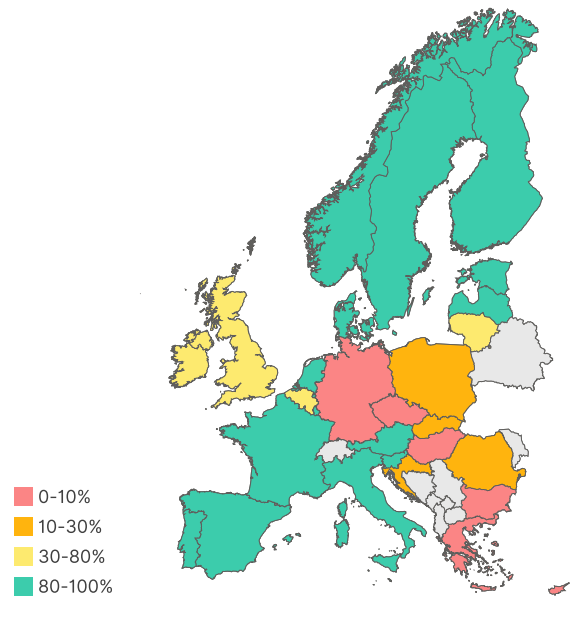
\includegraphics[width=0.75\linewidth]{figure/Smart_EU.PNG}
    \caption{Roll-out of smart meters among households \cite{ACER2024} }
    \label{fig:Smart_EU}
\end{figure}
     \end{center}
\end{column}
\begin{column}{0.50\textwidth}
\small	
 \boldrblue{20 EU countries out of 29} have regulated and non-regulated dynamic contract options for households \cite{ACER2024}
\hyperlink{ContractType}{\beamergotobutton{Table}},\hyperlink{USdata}{\beamergotobutton{US Data}},\hyperlink{options2}{\beamergotobutton{Details}},\hyperlink{UptakeContract2}{\beamergotobutton{Back }}
\hspace{2cm}
\end{column}
\end{columns}

\end{frame}


%%%%%%%%%%%%%%%%%%%%%%%%%%%%%%%%%%%%%%%%%%%%%%%%%%%%%%%%%%%%%%%%%%%%%%%%%%%%%%%%%%%%%%%%%%%%%%%%%%%%%%%%%%%%%%%%%%%%%%%%%%%%%%%%%%%%%%%%%%%%%%%%%%%%%%

\begin{frame}{Available technology and contract options}\label{options2}

% \begin{columns}

% \begin{column}{0.55\textwidth}  %%<--- here
%     \begin{center}
% \begin{figure}
%     \centering
%     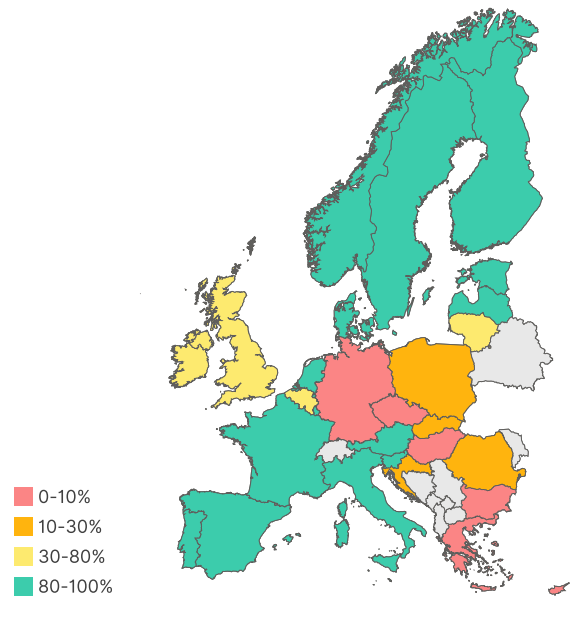
\includegraphics[width=0.75\linewidth]{figure/Smart_EU.PNG}
%     \caption{Roll-out of smart meters among households \cite{ACER2024} }
%     \label{fig:Smart_EU}
% \end{figure}
%      \end{center}
% \end{column}
% \begin{column}{0.50\textwidth}
% \small	
%  \boldrblue{20 EU countries out of 29} have regulated and non-regulated dynamic contract options for households \cite{ACER2024}

% \hspace{2cm}

\begin{figure}
    \centering
    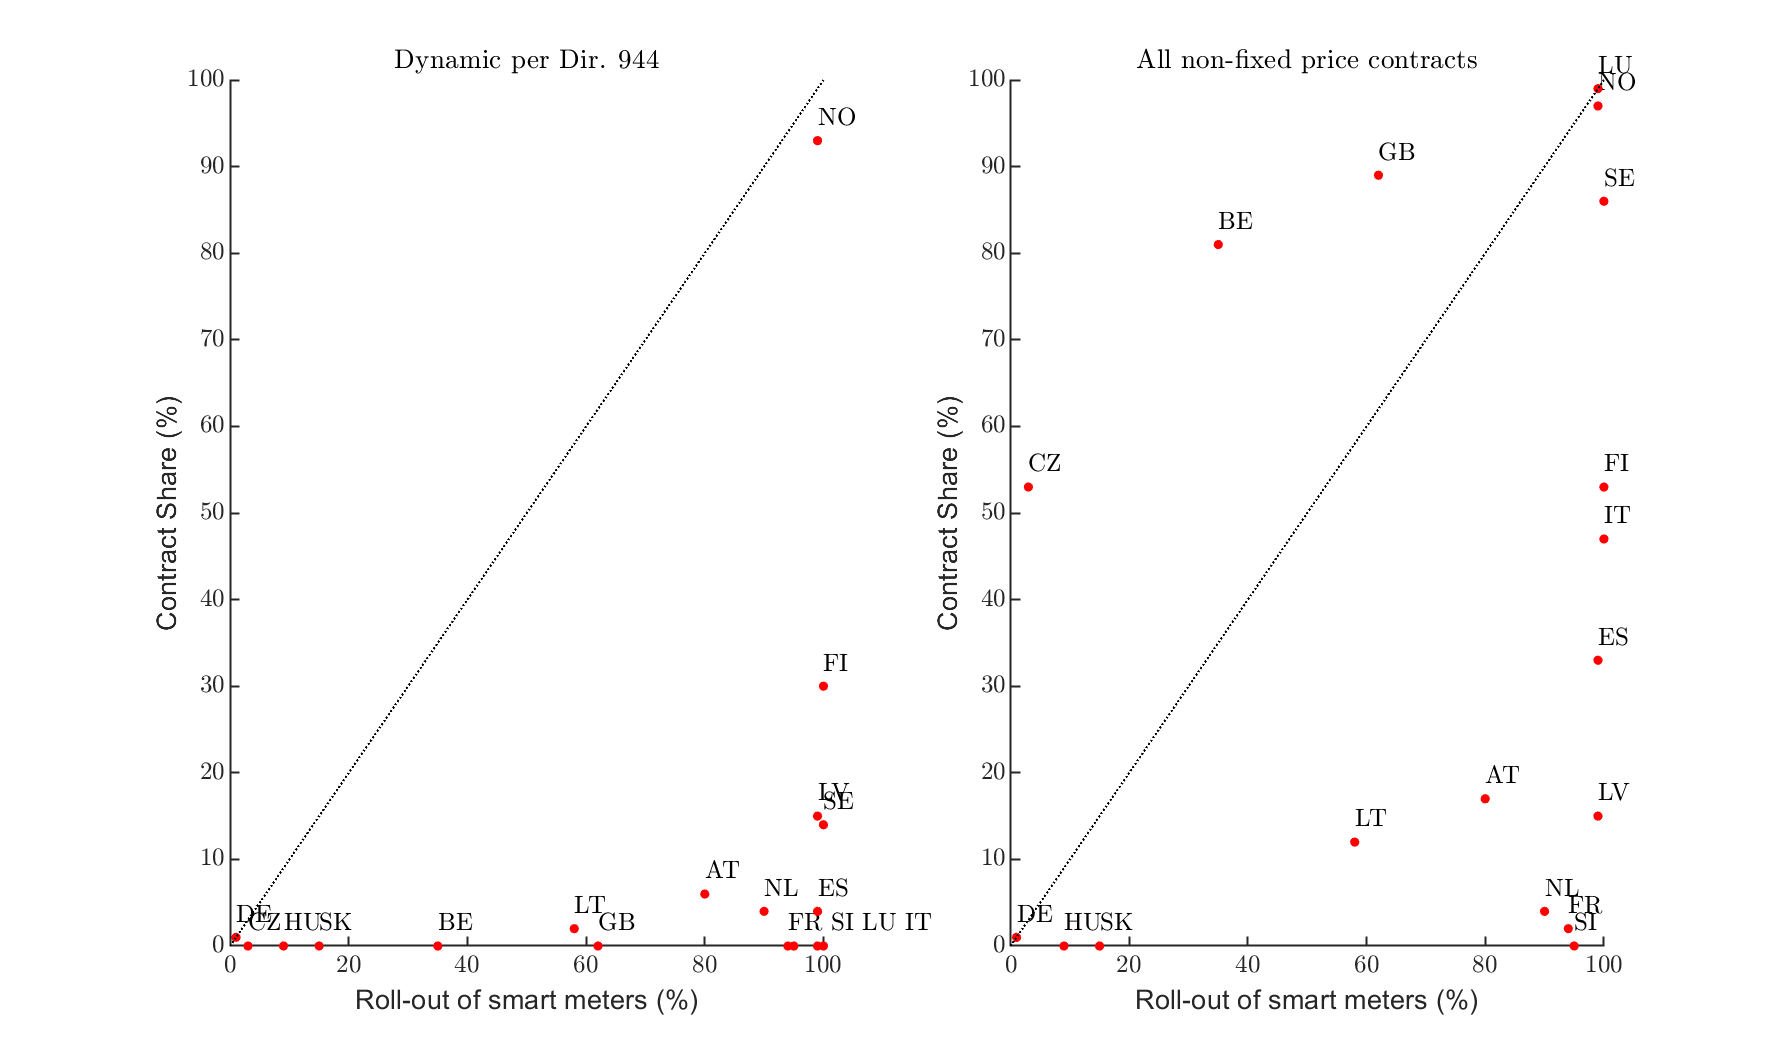
\includegraphics[width=1\linewidth]{figure/share_contract.PNG}
    \caption{Share of contract uptakes with respect to share of roll-out of smart meters among households (own calculation based on \cite{ACER2024}),\hyperlink{ContractType}{\beamergotobutton{Table}},\hyperlink{USdata}{\beamergotobutton{US Data}},\hyperlink{options1}{\beamergotobutton{Back}}}
    \label{fig:Smart_EU}
\end{figure}







% \end{column}
% \end{columns}



\end{frame}


%%%%%%%%%%%%%%%%%%%%%%%%%%
%%%%%%%%%%%%%%%%%%%%%%%%%%%%%%%%%%%%%%%%%%%%%%%%%%%%%%%%%%%%%%%%%%%%%%%%%%%%%%%%%%%%%%%%%%%%%%%%%%%%%%%%%%%%%%%%%%%%%%%%%%%%%%%%%%%%%%%%%%%%%%%%%%%%%%

\begin{frame}{Contract Options in the EU}\label{ContractType}

\begin{figure}
    \centering
    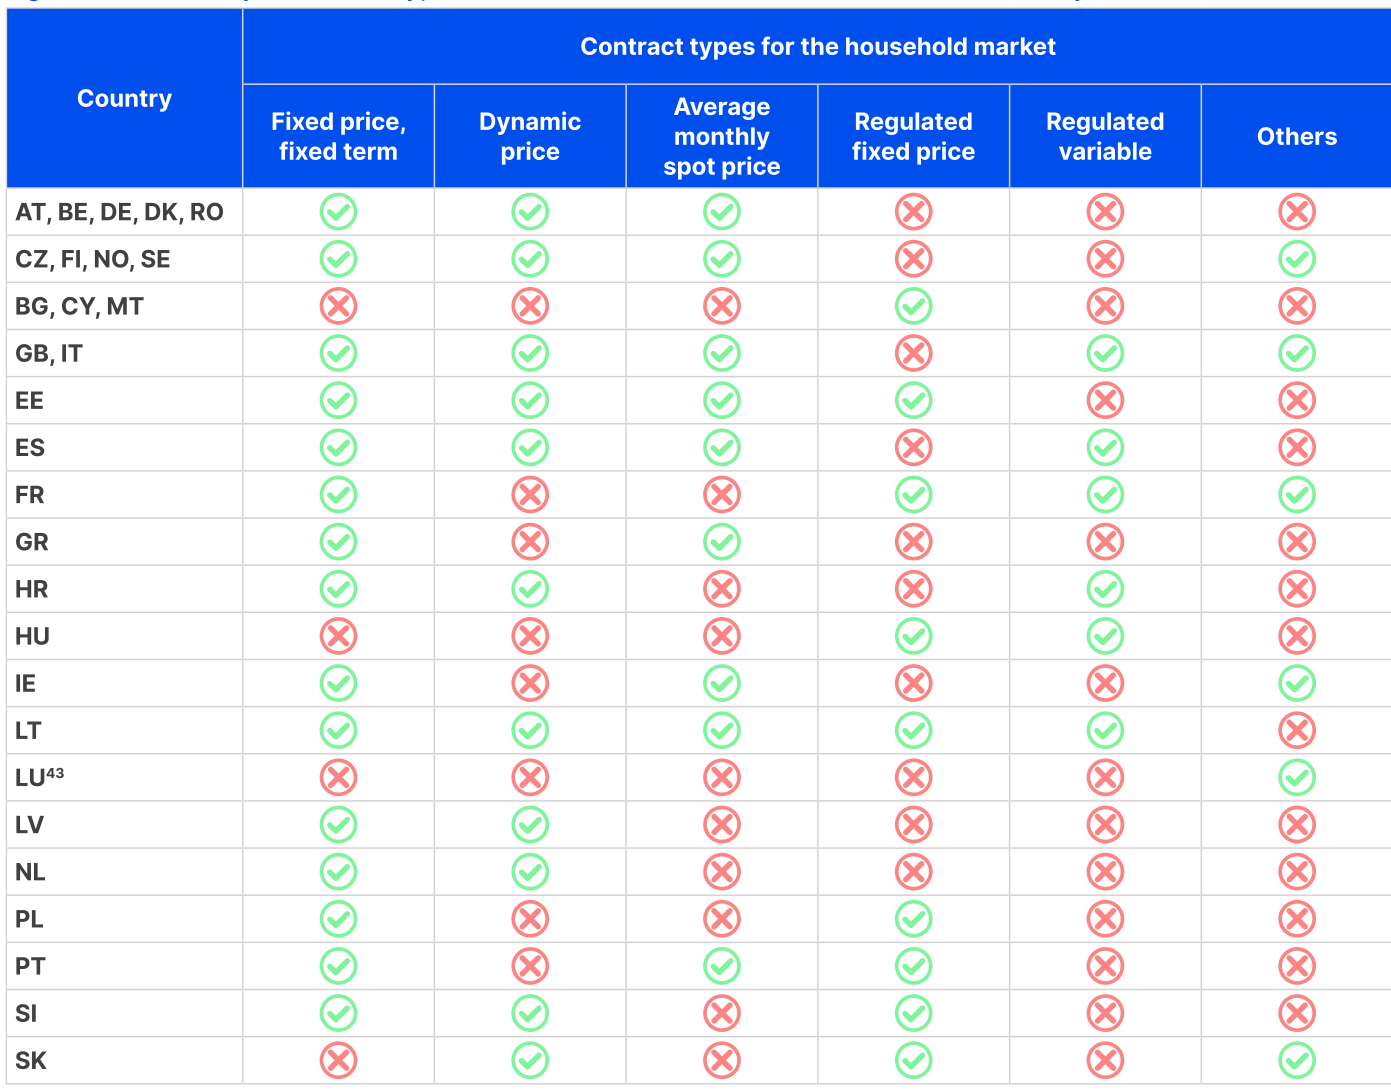
\includegraphics[width=0.8\linewidth]{figure/ContractType.PNG}
    \caption{Availability of different types of contracts to customers in the household electricity market in 2023 Country.\cite{ACER2024}  \hyperlink{options1}{\beamergotobutton{Back}} }
    \label{fig:ContractType}
\end{figure}
    
\end{frame}


%%%%%%%%%%%%%%%%%%%%%%%%%%%%%%%%%%%%%%%%%%%%%%%%%%%%%%%%%%%%%%%%%%%%%%%%%%%%%%%%%%%%%%%%%%%%%%%%%%%%%%%%%%%%%%%%%%%%%%%%%%%%%%%%%%%%%%%%%%%%%%%%%%%%%%

\begin{frame}{US Data}\label{USdata}

\begin{figure}
    \centering
    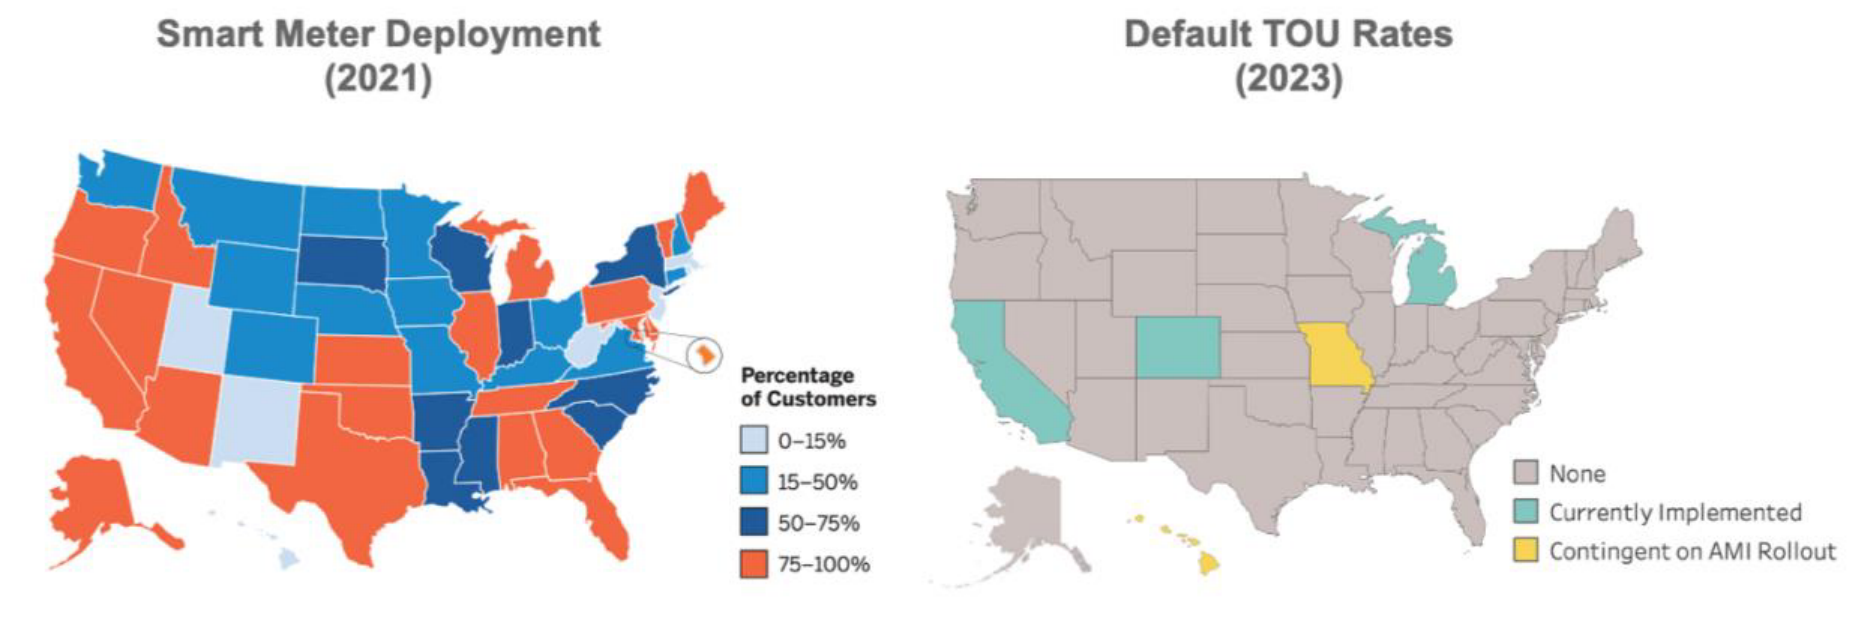
\includegraphics[width=1\linewidth]{figure/FP_Smart_US.PNG}
    \caption{Smart meter deployment among US households (left) and default TOU rate adoption (right). Default TOU rates are shown for each state's largest distribution utility. \cite{Turk2024}  \hyperlink{options1}{\beamergotobutton{Back}} }
    \label{fig:FP_Smart_US}
\end{figure}
    
\end{frame}

%%%%%%%%%%%%%%%%%%%%%%%%%%%%%%%%%%%%%%%%%%%%%%%%%%%%%%%%%%%%%%%%%%%%%%%%%%%%%%%%%%%%%%%%%%%%%%%%%%%%%%%%%%%%%%%%%%%%%%%%%%%%%%%%%%%%%%%%%%%%%%%%%%%%%%



\bibliography{bib}


\end{document}

\newlength{\tempb}

\frame{\titlepage}

\newcommand{\commentedbox}[2]{%
  \mbox{
    \begin{tabular}[t]{@{}c@{}}
    $\boxed{\displaystyle#1}$\\
    #2
    \end{tabular}%
  }%
}

\newcommand\Wider[2][3em]{%
\makebox[\linewidth][c]{%
  \begin{minipage}{\dimexpr\textwidth+#1\relax}
  \raggedright#2
  \end{minipage}%
  }%
}

\newcommand*\circled[1]{\tikz[baseline=(char.base)]{
            \node[shape=circle,draw,inner sep=2pt] (char) {#1};}}

%%%%%%%%%%%%%%%%%%%%%%%%%%%%%%%%%%%%%%%%%%%%%%%%%%%%%%%%%%%%%%%%%%%%%%%%%%%%%%%%%%%%%%%%%%%%%%%%%%%%%%%%%%%%%%%%%%%%%%%%%%%%%%%%%%%%%%%%%%%%%%%%%%%%%%

\section{Introduction and motivations}


\begin{frame}{Motivations}\label{Motivations}

\begin{mainbox}{Questions}
\begin{itemize}
\vspace{0.15 cm}
    \item  How do heterogeneous consumers self-select into different contracts?
        \vspace{0.15 cm}
    \item How does this sorting interact with market equilibrium?
(\textit{private vs. public provision})
    \vspace{0.15 cm}
\end{itemize}
\end{mainbox}

\vfill

\begin{itemize}    
    \item Focus on \boldrblue{electricity markets}: Fixed Price vs. Dynamic Price contract. \vfill
    
    \item \boldrblue{First Best.} Consumers should face the real-time marginal cost. \vfill
    
    \item \boldrblue{Moral hazard.} Different contract choices imply allocative inefficiencies.
\end{itemize}

       
\end{frame}

%%%%%%%%%%%%%%%%%%%%%%%%%%%%%%%%%%%%%%%%%%%%%%%%%%%%%%%%%%%%%%%%%%%%%%%%%%%%%%%%%%%%%%%%%%%%%%%%%%%%%%%%%%%%%%%%%%%%%%%%%%%%%%%%%%%%%%%%%%%%%%%%%%%%%%

\begin{frame}{Private contracts coexist with regulated options }\label{UptakeContract2}

\begin{figure}
    \centering
    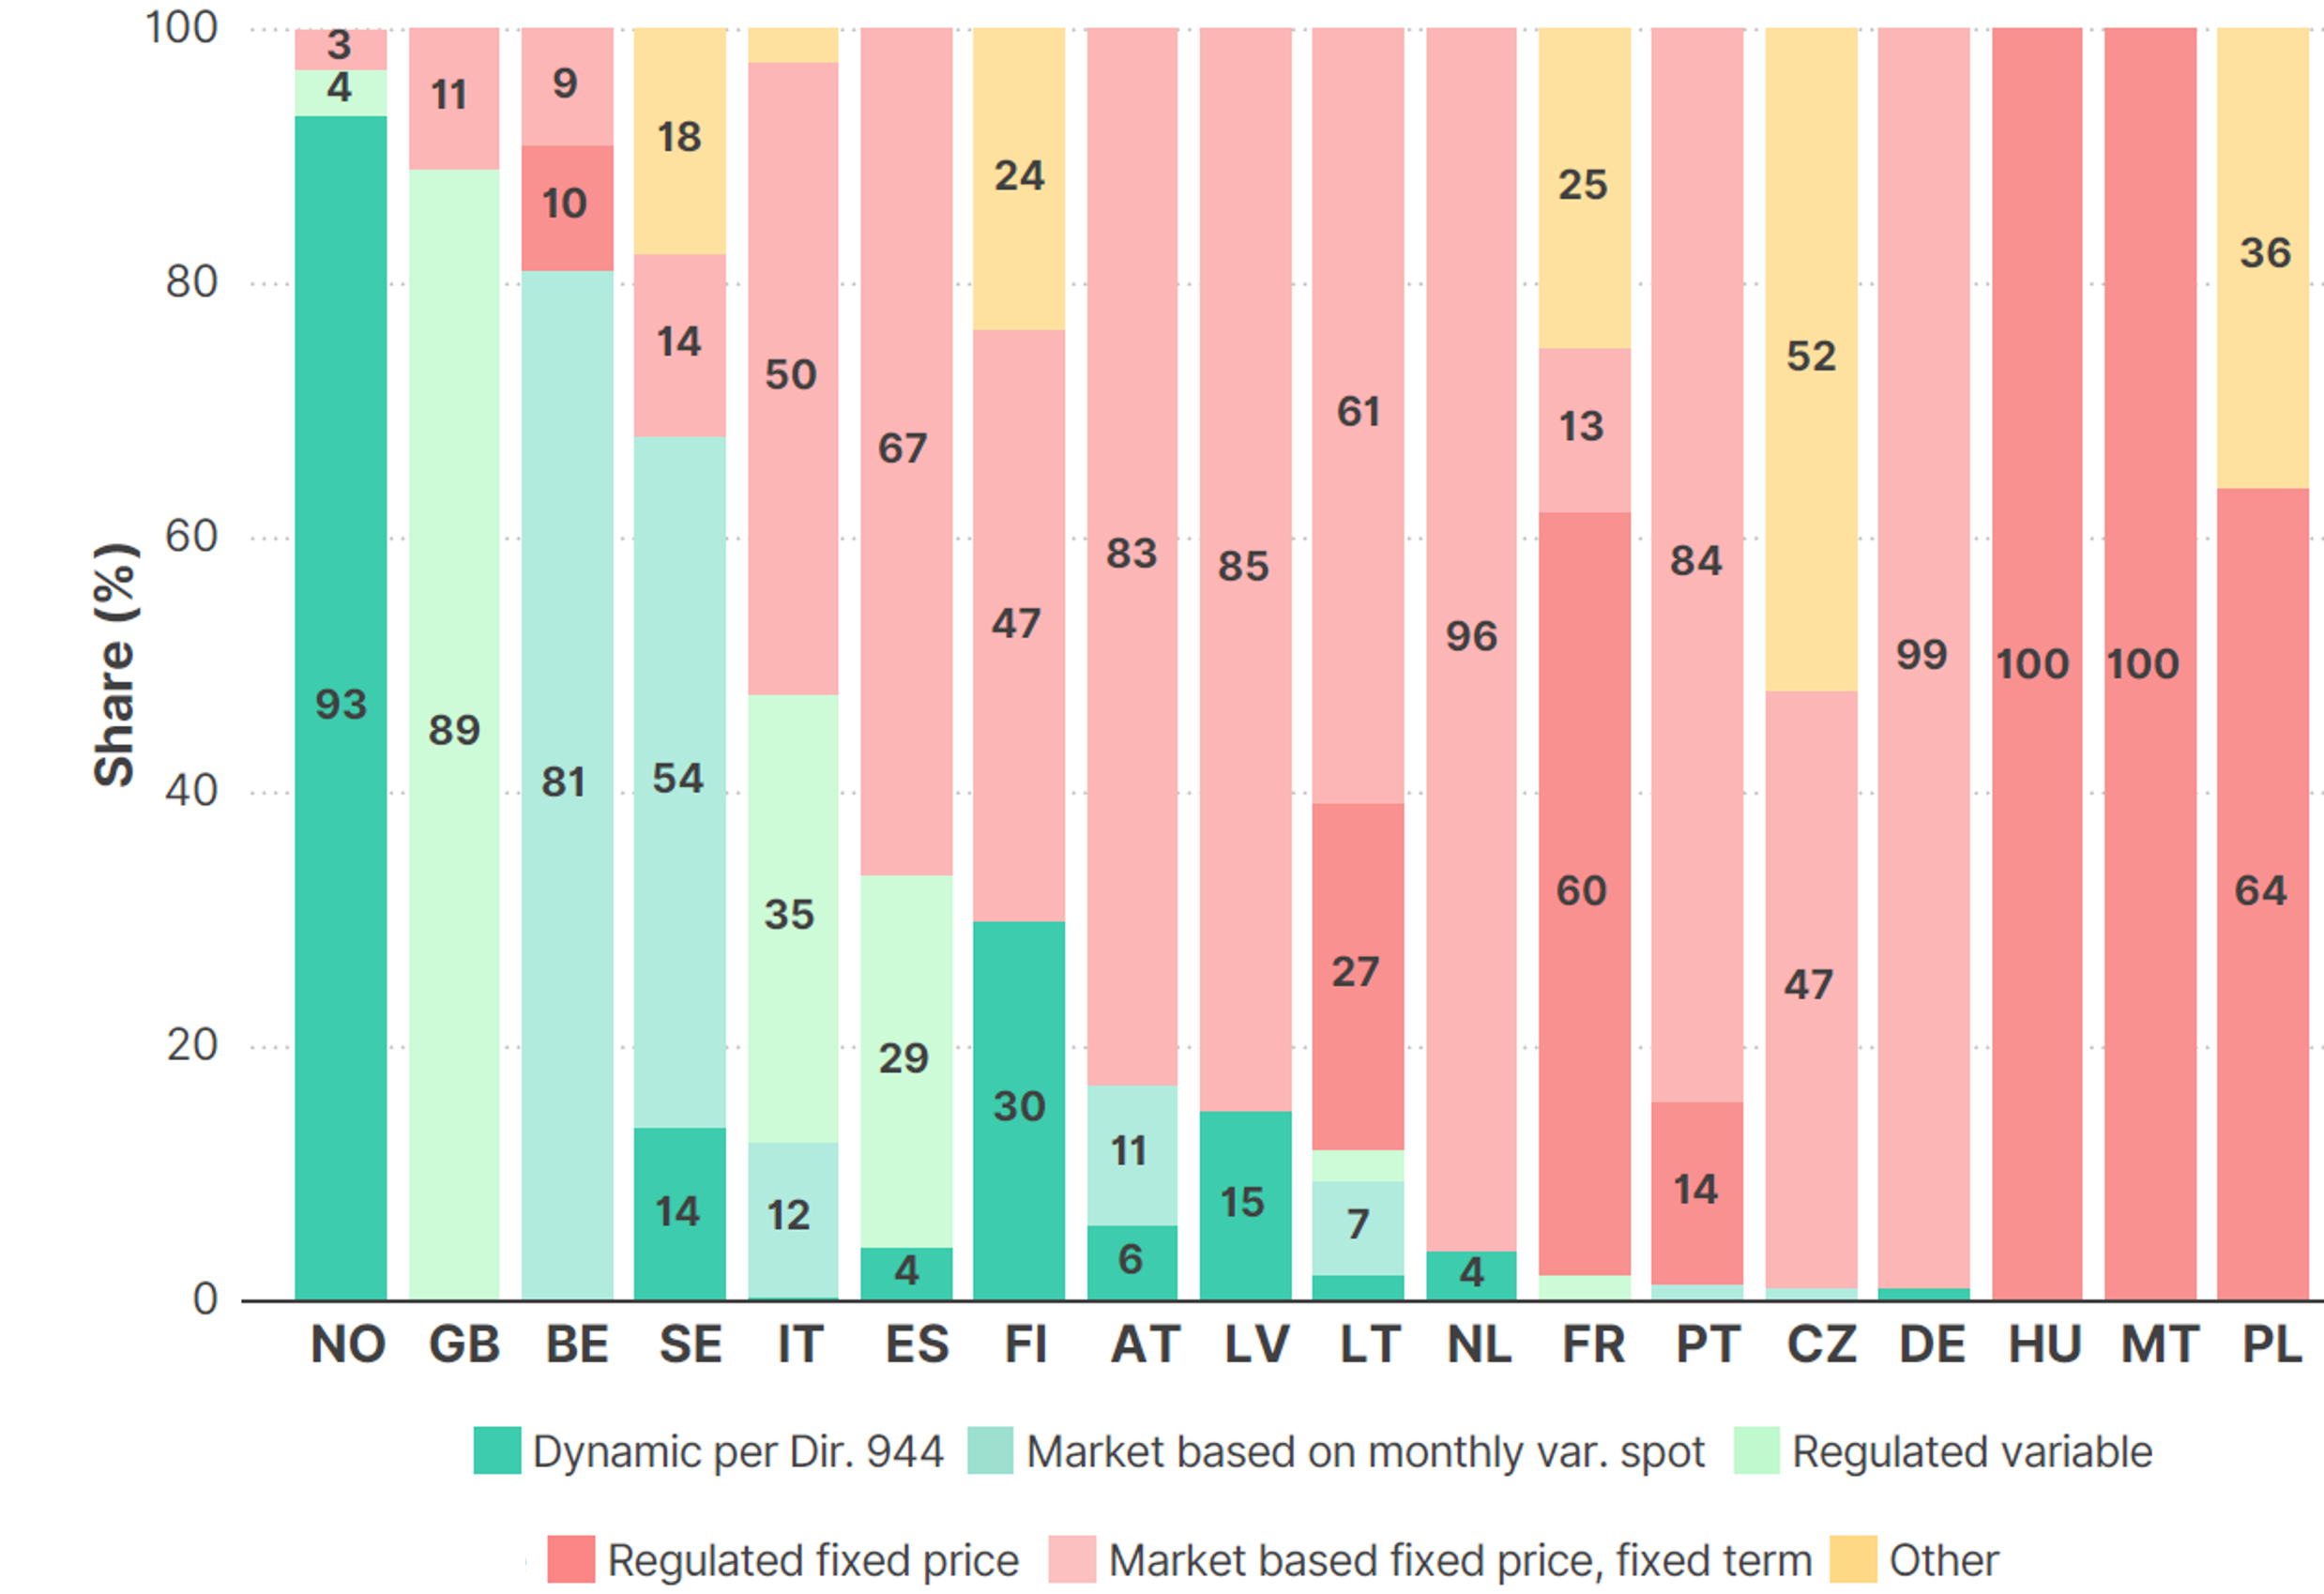
\includegraphics[width=0.8\linewidth]{figure/FP_EU_detail_v2.PNG}
    \caption{Share of household contract uptake in Europe \cite{ACER2024} \hyperlink{options1}{\beamergotobutton{Options}}} 
    \label{fig:FP_EU_detail}
\end{figure}

\end{frame}




%%%%%%%%%%%%%%%%%%%%%%%%%%%%%%%%%%%%%%%%%%%%%%%%%%%%%%%%%%%%%%%%%%%%%%%%%%%%%%%%%%%%%%%%%%%%%%%%%%%%%%%%%%%%%%%%%%%%%%%%%%%%%%%%%%%%%%%%%%%%%%%%%%%%%%



\begin{frame}{First contribution: Demand for contracts with heterogeneous consumers}\label{FirstCont}


\begin{itemize}

\item Provide a \boldrblue{stylized theoretical framework} where a set of consumers have to choose between \boldrblue{a Fixed-Price contract} or \boldrblue{a Dynamic-Price contract}. \vfill

\item Consumers can consume over \boldrblue{two periods} with \boldrblue{different willingness-to-pay} in each period (\textit{multidimensional}). 

\vfill

\item Assume entirely rational and risk-neutral consumers.

\vfill

\end{itemize}

\begin{mainbox}{Partial Equilibrium}
Provide \boldrblue{the demand} for each contract, given a set of prices and the type of consumers who choose each contract.  
\end{mainbox}

\vfill

\begin{itemize}

\item Literature \hyperlink{Lit_Conso}{\beamergotobutton{Contracts and Electricity Markets}} 
\end{itemize}



\end{frame}



%%%%%%%%%%%%%%%%%%%%%%%%%%%%%%%%%%%%%%%%%%%%%%%%%%%%%%%%%%%%%%%%%%%%%%%%%%%%%%%%%%%%%%%%%%%%%%%%%%%%%%%%%%%%%%%%%%%%%%%%%%%%%%%%%%%%%%%%%%%%%%%%%%%%%%



\begin{frame}{Second contribution: Market equilibrium with consumer choices}\label{SecondCont}


\begin{itemize}

\item We model \boldrblue{retail competition} between firms that offer the two contracts. 

\vfill

\item Focus on \boldrblue{price equilibrium}.

\vfill

\item The \boldrblue{market structure} is composed of two types of firms. \vfill

\begin{itemize}
    \item Perfectly competitive retailers and a regulated firm.
\end{itemize}

\end{itemize}


\vfill

\begin{mainbox}{General Equilibrium}
We characterize \boldrblue{the price and welfare equilibrium} in the retail market when consumers can self-select.
\end{mainbox}

\vfill

\begin{itemize}
\item Literature \hyperlink{Lit_Mkt1}{\beamergotobutton{Retail Competition in Electricity Markets}}  and \hyperlink{Lit_Mkt2}{\beamergotobutton{General Theory}} 
\end{itemize}


\end{frame}

%%%%%%%%%%%%%%%%%%%%%%%%%%%%%%%%%%%%%%%%%%%%%%%%%%%%%%%%%%%%%%%%%%%%%%%%%%%%%%%%%%%%%%%%%%%%%%%%%%%%%%%%%%%%%%%%%%%%%%%%%%%%%%%%%%%%%%%%%%%%%%%%%%%%%%

\begin{frame}{Main takeaways}


\begin{itemize}

\item \boldrblue{A selection model}. heterogeneity and multidimensionality of types $\rightarrow$ retail cost depends on consumer types.


\vfill

\item \boldrblue{Optimal demand for contracts}: Higher willingness to pay during low-price periods $\rightarrow$ dynamic contract. Opposite for the fixed-price contract.

\vfill

\item \boldrblue{Market equilibrium}.

\vfill

\begin{itemize}
    \item At the equilibrium, a public firm may offer FP contract. \vfill

\item \boldrblue{Adverse selection}: \vfill

    \begin{center}
    $W$(\textcolor{blue}{Private} / \textcolor{blue}{Dynamic} + \textcolor{red}{Public} / \textcolor{red}{Fixed-Price})  { \textbf{  < }} $W$( \textcolor{red}{Fixed-Price})
   \end{center}

\vfill

\item Leakage of consumers to the private firms $\rightarrow$ low equilibrium fixed-price.

    \end{itemize}

\end{itemize}


\end{frame}






%%%%%%%%%%%%%%%%%%%%%%%%%%%%%%%%%%%%%%%%%%%%%%%%%%%%%%%%%%%%%%%%%%%%%%%%%%%%%%%%%%%%%%%%%%%%%%%%%%%%%%%%%%%%%%%%%%%%%%%%%%%%%%%%%%%%%%%%%%%%%%%%%%%%%%
%%%%%%%%%%%%%%%%%%%%%%%%%%%%%%%%%%%%%%%%%%%%%%%%%%%%%%%%%%%%%%%%%%%%%%%%%%%%%%%%%%%%%%%%%%%%%%%%%%%%%%%%%%%%%%%%%%%%%%%%%%%%%%%%%%%%%%%%%%%%%%%%%%%%%%
%%%%%%%%%%%%%%%%%%%%%%%%%%%%%%%%%%%%%%%%%%%%%%%%%%%%%%%%%%%%%%%%%%%%%%%%%%%%%%%%%%%%%%%%%%%%%%%%%%%%%%%%%%%%%%%%%%%%%%%%%%%%%%%%%%%%%%%%%%%%%%%%%%%%%%

\section{The model}

% \subsection{The environment}

\begin{frame}{Roadmap}
  \tableofcontents [sectionstyle=show/shaded,subsectionstyle=show/shaded]
\end{frame}


%%%%%%%%%%%%%%%%%%%%%%%%%%%%%%%%%%%%%%%%%%%%%%%%%%%%%%%%%%%%%%%%%%%%%%%%%%%%%%%%%%%%%%%%%%%%%%%%%%%%%%%%%%%%%%%%%%%%%%%%%%%%%%%%%%%%%%%%%%%%%%%%%%%%%%


\begin{frame}{Timing}


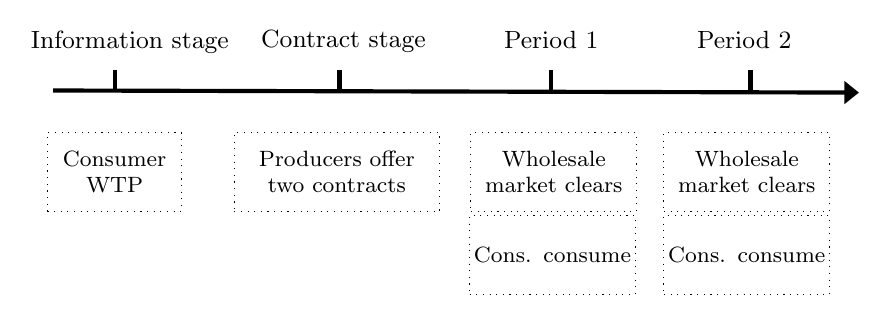
\begin{tikzpicture}[x=0.45pt,y=0.75pt,yscale=-1,xscale=1]

\draw [line width=1.5]    (20,100) -- (663,101) ;
\draw [shift={(667,101)}, rotate = 180.07] [fill={rgb, 255:red, 0; green, 0; blue, 0 }  ][line width=0.08]  [draw opacity=0] (11.61,-5.58) -- (0,0) -- (11.61,5.58) -- cycle    ;
\draw [line width=1.5,color = black]    (70,90) -- (70,100) ;
\draw [line width=1.5,color = black]   (250,90) -- (250,100) ;
\draw [line width=1.5,color = black]   (420,90) -- (420,100)  ;
\draw [line width=1.5,color = black]    (580,90) -- (580,100)   ;

% Text Node
\draw (0,70) node [anchor=north west][inner sep=0.75pt]  [font=\small] [align=center] {Information stage};
\draw (185,70) node [anchor=north west][inner sep=0.75pt]  [font=\small] [align=center] {Contract  stage};
\draw (380,70) node [anchor=north west][inner sep=0.75pt]  [font=\small] [align=center] {Period 1};
\draw (535,70) node [anchor=north west][inner sep=0.75pt]  [font=\small] [align=center] {Period 2};

\draw (15,120) node [draw = black,anchor=north west,minimum height = 1 cm,  text  width = 1.6cm][inner sep=1.5pt,dotted]  [font=\footnotesize] [align=center] {Consumer WTP};
% \draw (15,160) node [anchor=north west,minimum height = 1 cm,  text  width = 1.6cm,dotted][inner sep=1.5pt]  [font=\footnotesize] [align=center] { \textit{common info.} \\ \textit{private info.}};

\draw (165,120) node [draw = black,anchor=north west,minimum height = 1 cm,  text  width = 2.5cm][inner sep=1.5pt,dotted]  [font=\footnotesize] [align=center]{ Producers offer \\ two contracts};
\draw (355,120) node [draw = black,anchor=north west,minimum height = 1 cm,  text  width =  2cm,dotted][inner sep=1.5pt]  [font=\footnotesize] [align=center] { Wholesale  \\ market clears};
\draw (354,160) node [draw = black,anchor=north west,minimum height = 1 cm,  text  width = 2cm,dotted][inner sep=1.5pt]  [font=\footnotesize] [align=center] { Cons. consume};

\draw (510,120) node [draw = black,anchor=north west,minimum height = 1 cm,  text  width = 2cm,dotted][inner sep=1.5pt]  [font=\footnotesize] [align=center] { Wholesale  \\ market clears};
\draw (510,160) node [draw = black,anchor=north west,minimum height = 1 cm,  text  width = 2cm,dotted][inner sep=1.5pt]  [font=\footnotesize] [align=center] { Cons. consume};

\end{tikzpicture}

    
\end{frame}



%%%%%%%%%%%%%%%%%%%%%%%%%%%%%%%%%%%%%%%%%%%%%%%%%%%%%%%%%%%%%%%%%%%%%%%%%%%%%%%%%%%%%%%%%%%%%%%%%%%%%%%%%%%%%%%%%%%%%%%%%%%%%%%%%%%%%%%%%%%%%%%%%%%%%%

\begin{frame}{Consumers}

\begin{itemize}
    \item A unit mass of consumers.

\vfill

    \item With a \boldrblue{unit demand} for electricity for each two periods $t = 1,2$.

\vfill

    \item W.t.p: a \boldrblue{two-dimensional} type $\textbf{v}=(v_1,v_2) $
    
\vfill

        % \begin{itemize}
 \item Drawn from a pdf. $f_t(v)$ and cdf. $F_t(v)$ with support $[\underline{v}_t,\bar{v}_t]$. 
            
% \vfill

        % \item Even though the distributions are independent, we assume the affine relationship between the two periods, where $\alpha,\beta \in \mathbb{R}$.

% \end{itemize}

        % \begin{equation*}
        %     [ \ubar{v}_2, \bar{v}_2] = [\alpha + \beta \ubar{v}_1, \alpha + \beta \bar{v}_1]
        % \end{equation*}


\vfill

\item Type $\textbf{v}$ consumer surplus from consuming at price profile $\textbf{p}$ is:

\begin{equation*}
 u\left(\textbf{v},\textbf{p}\right)= v_1-p_1 +  v_2-p_2
 \end{equation*}
\end{itemize}    
\end{frame}

%%%%%%%%%%%%%%%%%%%%%%%%%%%%%%%%%%%%%%%%%%%%%%%%%%%%%%%%%%%%%%%%%%%%%%%%%%%%%%%%%%%%%%%%%%%%%%%%%%%%%%%%%%%%%%%%%%%%%%%%%%%%%%%%%%%%%%%%%%%%%%%%%%%%%%

\begin{frame}{Wholesale market}


\begin{itemize}
    \item \boldrblue{Perfectly competitive firms} produce each periods $q$ unit of electricity at a linear production cost: 
\end{itemize}

\begin{equation*}
    C_t(q) = c_t q
\end{equation*}

\vfill

\begin{itemize}
    \item We assume w.l.o.g. that $c_1 < c_2$

\vfill

\begin{itemize}
    \item Off-peak period: $t = 1$ and On-peak period: $t = 2$. \vfill
    \item Due to perfect competition: $\textbf{p}_w = \{p_1^w,p_2^w\} = \{c_1,c_2\}$.
\end{itemize}

\vfill

\item Period 1 is a sunny afternoon with renewable production with null marginal cost, and period 2 is the evening with fuel producers with high marginal cost.


\vfill

\item  No uncertainty, no investment decision, and no capacity constraints.

\end{itemize}
    
\end{frame}

%%%%%%%%%%%%%%%%%%%%%%%%%%%%%%%%%%%%%%%%%%%%%%%%%%%%%%%%%%%%%%%%%%%%%%%%%%%%%%%%%%%%%%%%%%%%%%%%%%%%%%%%%%%%%%%%%%%%%%%%%%%%%%%%%%%%%%%%%%%%%%%%%%%%%%

\begin{frame}{Retailers}

\begin{itemize}
    \item We assume a set of retailers that purchase at no cost on the wholesale market.

    \vfill

    \item We take the characteristics of contracts and the set of contracts as given.  \vfill
    
    \item If $\textbf{p}_k=(p_1^k,p_2^k)$ is profile unit-price of contract $k$, then:  \vfill

    \begin{itemize}
        \item FP contract: $\textbf{p}_{r} =  (p^r,p^r)$ \vfill
        \item Dynamic contract: $\textbf{p}_{s} =  (p_1,p_2)$ \vfill
    \end{itemize}

\item $A_k$ is the fixed-part of a two-parts tariff. 


\end{itemize}


    
\end{frame}

%%%%%%%%%%%%%%%%%%%%%%%%%%%%%%%%%%%%%%%%%%%%%%%%%%%%%%%%%%%%%%%%%%%%%%%%%%%%%%%%%%%%%%%%%%%%%%%%%%%%%%%%%%%%%%%%%%%%%%%%%%%%%%%%%%%%%%%%%%%%%%%%%%%%%%


\begin{frame}{Equilibrium Definition}


\begin{itemize}

\item The optimal consumer choose a consumption profile $\textbf{x} = (x_1,x_2)$ with $x_t =\{0,1\}$, given a contract, to maximize its utility:

\vfill

\begin{equation*}
U\left(\textbf{v},\textbf{p}_k, A_k\right) \quad = \quad  \max_{\textbf{x}} \quad \textbf{x} (\textbf{v} - \textbf{p}_k) - A_k \; \textbf{1}_{x_1 + x_2 \geq 1} 
\end{equation*}

\vfill
    
\item Given a contract $k$, a \textit{private firm} equilibrium is such that:

\vfill

\begin{equation*}
 \pi_k(\textbf{p}_{k},A_k) = \textbf{q}_k (\textbf{p}_k - \textbf{p}_w) + \mu_k A_k  =0 
\end{equation*}

\vfill

\item A \textit{public firm} equilibrium is such that:

\vfill

\begin{equation*}
 \max \quad CS^r(\textbf{p}_r,A_r) + (1+\lambda)\pi_r(\textbf{p}_{r},A_r)
\end{equation*}

\end{itemize}

{\footnotesize $\mu_k = $ mass of consumers}
    
\end{frame}
%%%%%%%%%%%%%%%%%%%%%%%%%%%%%%%%%%%%%%%%%%%%%%%%%%%%%%%%%%%%%%%%%%%%%%%%%%%%%%%%%%%%%%%%%%%%%%%%%%%%%%%%%%%%%%%%%%%%%%%%%%%%%%%%%%%%%%%%%%%%%%%%%%%%%%


\begin{frame}{The single contract case}

\begin{figure}
    \centering
    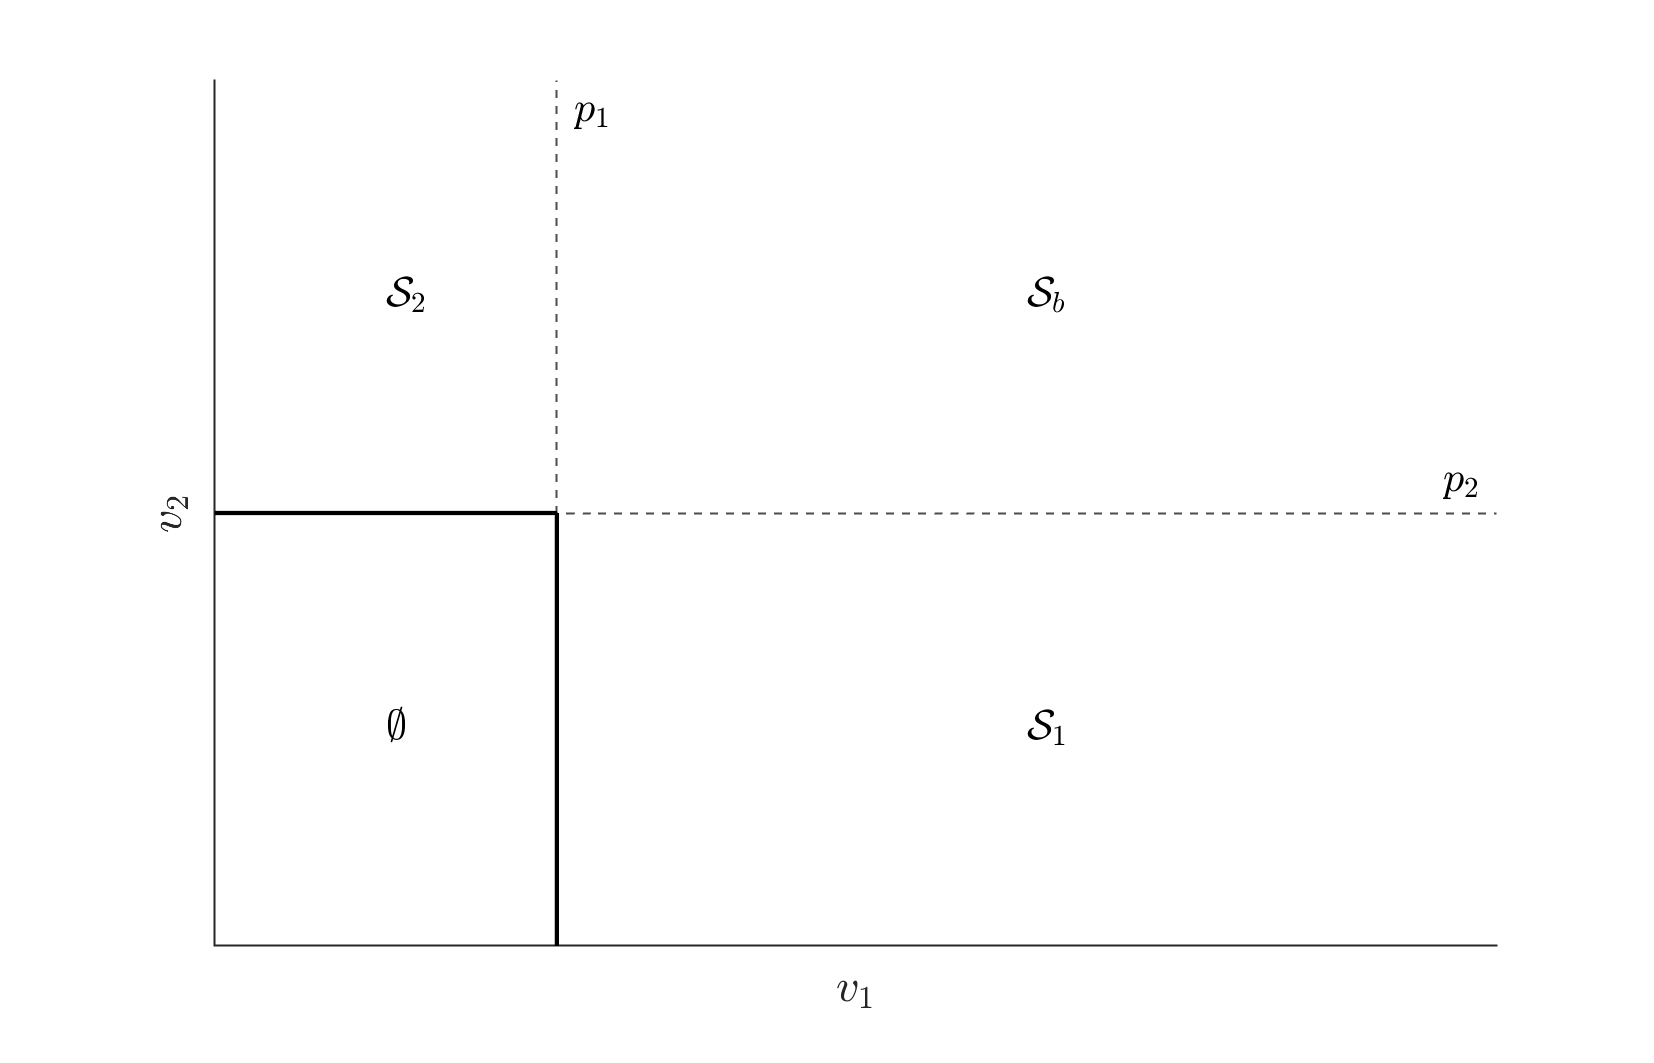
\includegraphics[width=0.8\linewidth]{figure/spot_demand_multi.png}
     \caption{The canonical bundle case.} 
    \label{fig:spot_demand_multi}
\end{figure}
    
    
\end{frame}
%%%%%%%%%%%%%%%%%%%%%%%%%%%%%%%%%%%%%%%%%%%%%%%%%%%%%%%%%%%%%%%%%%%%%%%%%%%%%%%%%%%%%%%%%%%%%%%%%%%%%%%%%%%%%%%%%%%%%%%%%%%%%%%%%%%%%%%%%%%%%%%%%%%%%%

% \begin{frame}{Single Contract Equilibrium}

% \begin{itemize}

% \item  \boldrblue{Private retailers - Dynamic only}, competition implies full cost pass-through:

% \vfill

% \begin{equation*}
%  \textbf{p}_s^*  = \{p_1^w,p_2^w\}  = \{c_1,c_2\}   \quad \text{and} \quad A_s^* =0 
% \end{equation*}

% \vfill

%  \item   \boldrblue{Private retailers - FP only},  linear price is the eq.:

% \begin{equation*}
%  p^r^{av} =  \underbrace{ p_1^w\frac{q_1^r}{q^r} + p_2^w \frac{q_2^r}{q^r} }_\text{av. retail cost}   \quad \text{and} \quad A_r^* =0 
% \end{equation*}

% \vfill



% \item \boldrblue{Public firm - FP only}, then the equilibrium is a Ramsey formula: 


%         \begin{equation*}
%             p^r^{**}  =\underbrace{\bigg.\frac{\lambda}{1+\lambda}\frac{q^r}{ \delta_A q^r}\left(1 - \frac{1}{\mu_r/q^r}\right)\bigg.}_{\text{ramsey}} + \underbrace{\bigg.  p_1^w \frac{\delta_A q^r_1}{\delta_A q^r} + p^w_2\frac{\delta_A q^r_2}{\delta_A q^r} \bigg.}_{\text{multi. types} } + \underbrace{\bigg.A^{**}_r \frac{\delta_A\mu_r}{\delta_A q^r} \bigg.}_{\text{switchers wedge}}
%         \end{equation*}

% {\footnotesize $\delta_A x = \partial x/\partial A-\partial x/\partial p^r$, $\lambda$ budget shadow value.}

% \end{itemize}

% \end{frame}

%%%%%%%%%%%%%%%%%%%%%%%%%%%%%%%%%%%%%%%%%%%%%%%%%%%%%%%%%%%%%%%%%%%%%%%%%%%%%%%%%%%%%%%%%%%%%%%%%%%%%%%%%%%%%%%%%%%%%%%%%%%%%%%%%%%%%%%%%%%%%%%%%%%%%%



%%%%%%%%%%%%%%%%%%%%%%%%%%%%%%%%%%%%%%%%%%%%%%%%%%%%%%%%%%%%%%%%%%%%%%%%%%%%%%%%%%%%%%%%%%%%%%%%%%%%%%%%%%%%%%%%%%%%%%%%%%%%%%%%%%%%%%%%%%%%%%%%%%%%%%

% \begin{frame}{Adverse Selection in Single Contract Equilibrium}

% \begin{itemize}

% \item We derive sufficient and necessary conditions for the private and public equilibrium to exhibit adverse (or advantageous) selection.  \vfill

% \item  Private equilibrium (sufficient conditions): $p^r^{av} > p^r^{sb}$  \vfill

% \begin{equation*}
%  \frac{\# \text{marginal cons. in } t_1}{\# \text{ cons. in }t_1} > \frac{\# \text{marginal cons. in } t_2}{\# \text{ cons. in }t_2}   
% \end{equation*}

% \vfill

% \item  Public equilibrium (necessary conditions): $A < 0$    \vfill

% \begin{equation*}
%  \frac{\# \text{profile switchers in }t_1}{\# \text{ cons. in }t_1} <  (>)  \frac{\# \text{profile switchers in } t_2}{\# \text{cons. in }t_2}   \quad \text{and} \quad \lambda > (<)1 
% \end{equation*}

% \end{itemize}

% \end{frame}



%%%%%%%%%%%%%%%%%%%%%
%%%%%%%%%%%%%%%%%%%%%%%%%%%%%%%%%%%%%%%%%%%%%%%%%%%%%%%%%%%%%%%%%%%%%%%%%%%%%%%%%%%%%%%%%%%%%%%%%%%%%%%%%%%%%%%%%%%%%%%%%%%%%%%%%%%%%%%%%%%%%%%%%%%%%%

\section{Partial equilibrium: Demand for multiple contracts}


\begin{frame}{Roadmap}
  \tableofcontents [sectionstyle=show/shaded,subsectionstyle=show/shaded]
\end{frame}

%%%%%%%%%%%%%%%%%%%%%%%%%%%%%%%%%%%%%%%%%%%%%%%%%%%%%%%%%%%%%%%%%%%%%%%%%%%%%%%%%%%%%%%%%%%%%%%%%%%%%%%%%%%%%%%%%%%%%%%%%%%%%%%%%%%%%%%%%%%%%%%%%%%%%%



\begin{frame}{The marginal consumers}


\begin{itemize}

\item Partial equilibrium: contract prices as given: $p_1 < p^r < p_2$ \vfill


\item Marginal consumers $\equiv $ same utility over at least two options when optimizing over the set of contracts and consumption profiles.

\vfill

\item There are three types

\vfill

\begin{itemize}
    \item \textit{Exiters - stop consuming}\vfill
    \item \textit{Profile switchers - 2 periods vs 1 period in the same contract} \vfill
    \item Contract switchers - switch contract and consumption profile 
\end{itemize}



\end{itemize}

\end{frame}

%%%%%%%%%%%%%%%%%%%%%%%%%%%%%%%%%%%%%%%%%%%%%%%%%%%%%%%%%%%%%%%%%%%%%%%%%%%%%%%%%%%%%%%%%%%%%%%%%%%%%%%%%%%%%%%%%%%%%%%%%%%%%%%%%%%%%%%%%%%%%%%%%%%%%%


\begin{frame}{Illustration}\label{PlotIndifConso}

\begin{figure}
    \centering
    \includegraphics[width=1\linewidth]{figure/example_cstc_ppt.png}
     \caption{The three types of marginal consumers.} 
    \label{fig:example_conv_cstc_nocol}
\end{figure}
    
\end{frame}


%%%%%%%%%%%%%%%%%%%%%%%%%%%%%%%%%%%%%%%%%%%%%%%%%%%%%%%%%%%%%%%%%%%%%%%%%%%%%%%%%%%%%%%%%%%%%%%%%%%%%%%%%%%%%%%%%%%%%%%%%%%%%%%%%%%%%%%%%%%%%%%%%%%%%%

\begin{frame}{The demand for contracts}\label{ExogenousDemand}

\begin{figure}
    \centering
    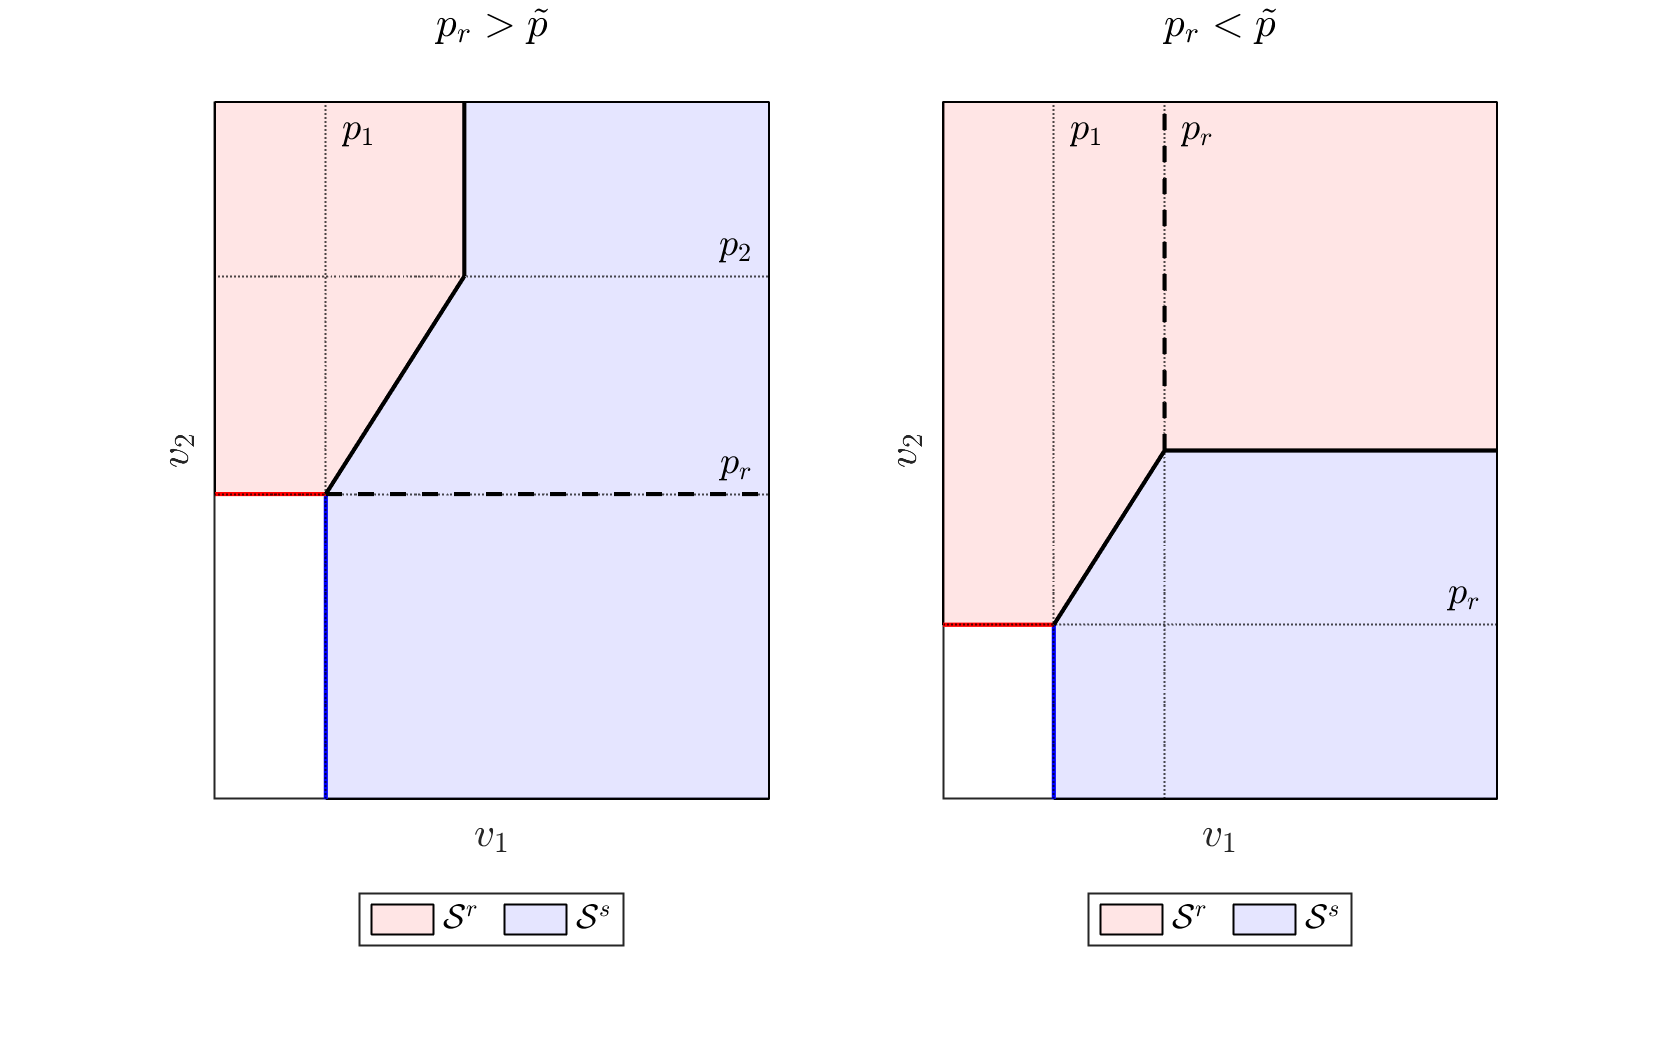
\includegraphics[width=1\linewidth]{figure/example_conv_cstc_ppt.png}
     \caption{The set of \textit{contract switchers} defines the mass of consumers choosing each contract.}
\end{figure}
    
\end{frame}


% \begin{frame}{Implication 2: The demand for electricity}\label{ExogenousDemand}

% \begin{figure}
%     \centering
%     \includegraphics[width=1\linewidth]{figure/example_conv_cqtt.png}
%      \caption{When $p^r < \Tilde{p}$ (resp. $p^r > \tilde{p}$ ), some consumers that choose the FP contract (resp. RTP contract) consume in both periods, while consumers under the RTP contracts (resp. FP contract) consume only during period 1 (resp. period 2).}
%     \label{fig:example_conv_cstc4}
% \end{figure}
    
% \end{frame}


%%%%%%%%%%%%%%%%%%%%%%%%%%%%%%%%%%%%%%%%%%%%%%%%%%%%%%%%%%%%%%%%%%%%%%%%%%%%%%%%%%%%%%%%%%%%%%%%%%%%%%%%%%%%%%%%%%%%%%%%%%%%%%%%%%%%%%%%%%%%%%%%%%%%%%
%%%%%%%%%%%%%%%%%%%%%%%%%%%%%%%%%%%%%%%%%%%%%%%%%%%%%%%%%%%%%%%%%%%%%%%%%%%%%%%%%%%%%%%%%%%%%%%%%%%%%%%%%%%%%%%%%%%%%%%%%%%%%%%%%%%%%%%%%%%%%%%%%%%%%%
%%%%%%%%%%%%%%%%%%%%%%%%%%%%%%%%%%%%%%%%%%%%%%%%%%%%%%%%%%%%%%%%%%%%%%%%%%%%%%%%%%%%%%%%%%%%%%%%%%%%%%%%%%%%%%%%%%%%%%%%%%%%%%%%%%%%%%%%%%%%%%%%%%%%%%

\section{General equilibrium: Retail contract prices}

\begin{frame}{Roadmap}
  \tableofcontents [sectionstyle=show/shaded,subsectionstyle=show/shaded]
\end{frame}



%%%%%%%%%%%%%%%%%%%%%%%%%%%%%%%%%%%%%%%%%%%%%%%%%%%%%%%%%%%%%%%%%%%%%%%%%%%%%%%%%%%%%%%%%%%%%%%%%%%%%%%%%%%%%%%%%%%%%%%%%%%%%%%%%%%%%%%%%%%%%%%%%%%%%%

\begin{frame}{Incentive for fixed-price contract}

\begin{figure}
    \centering
    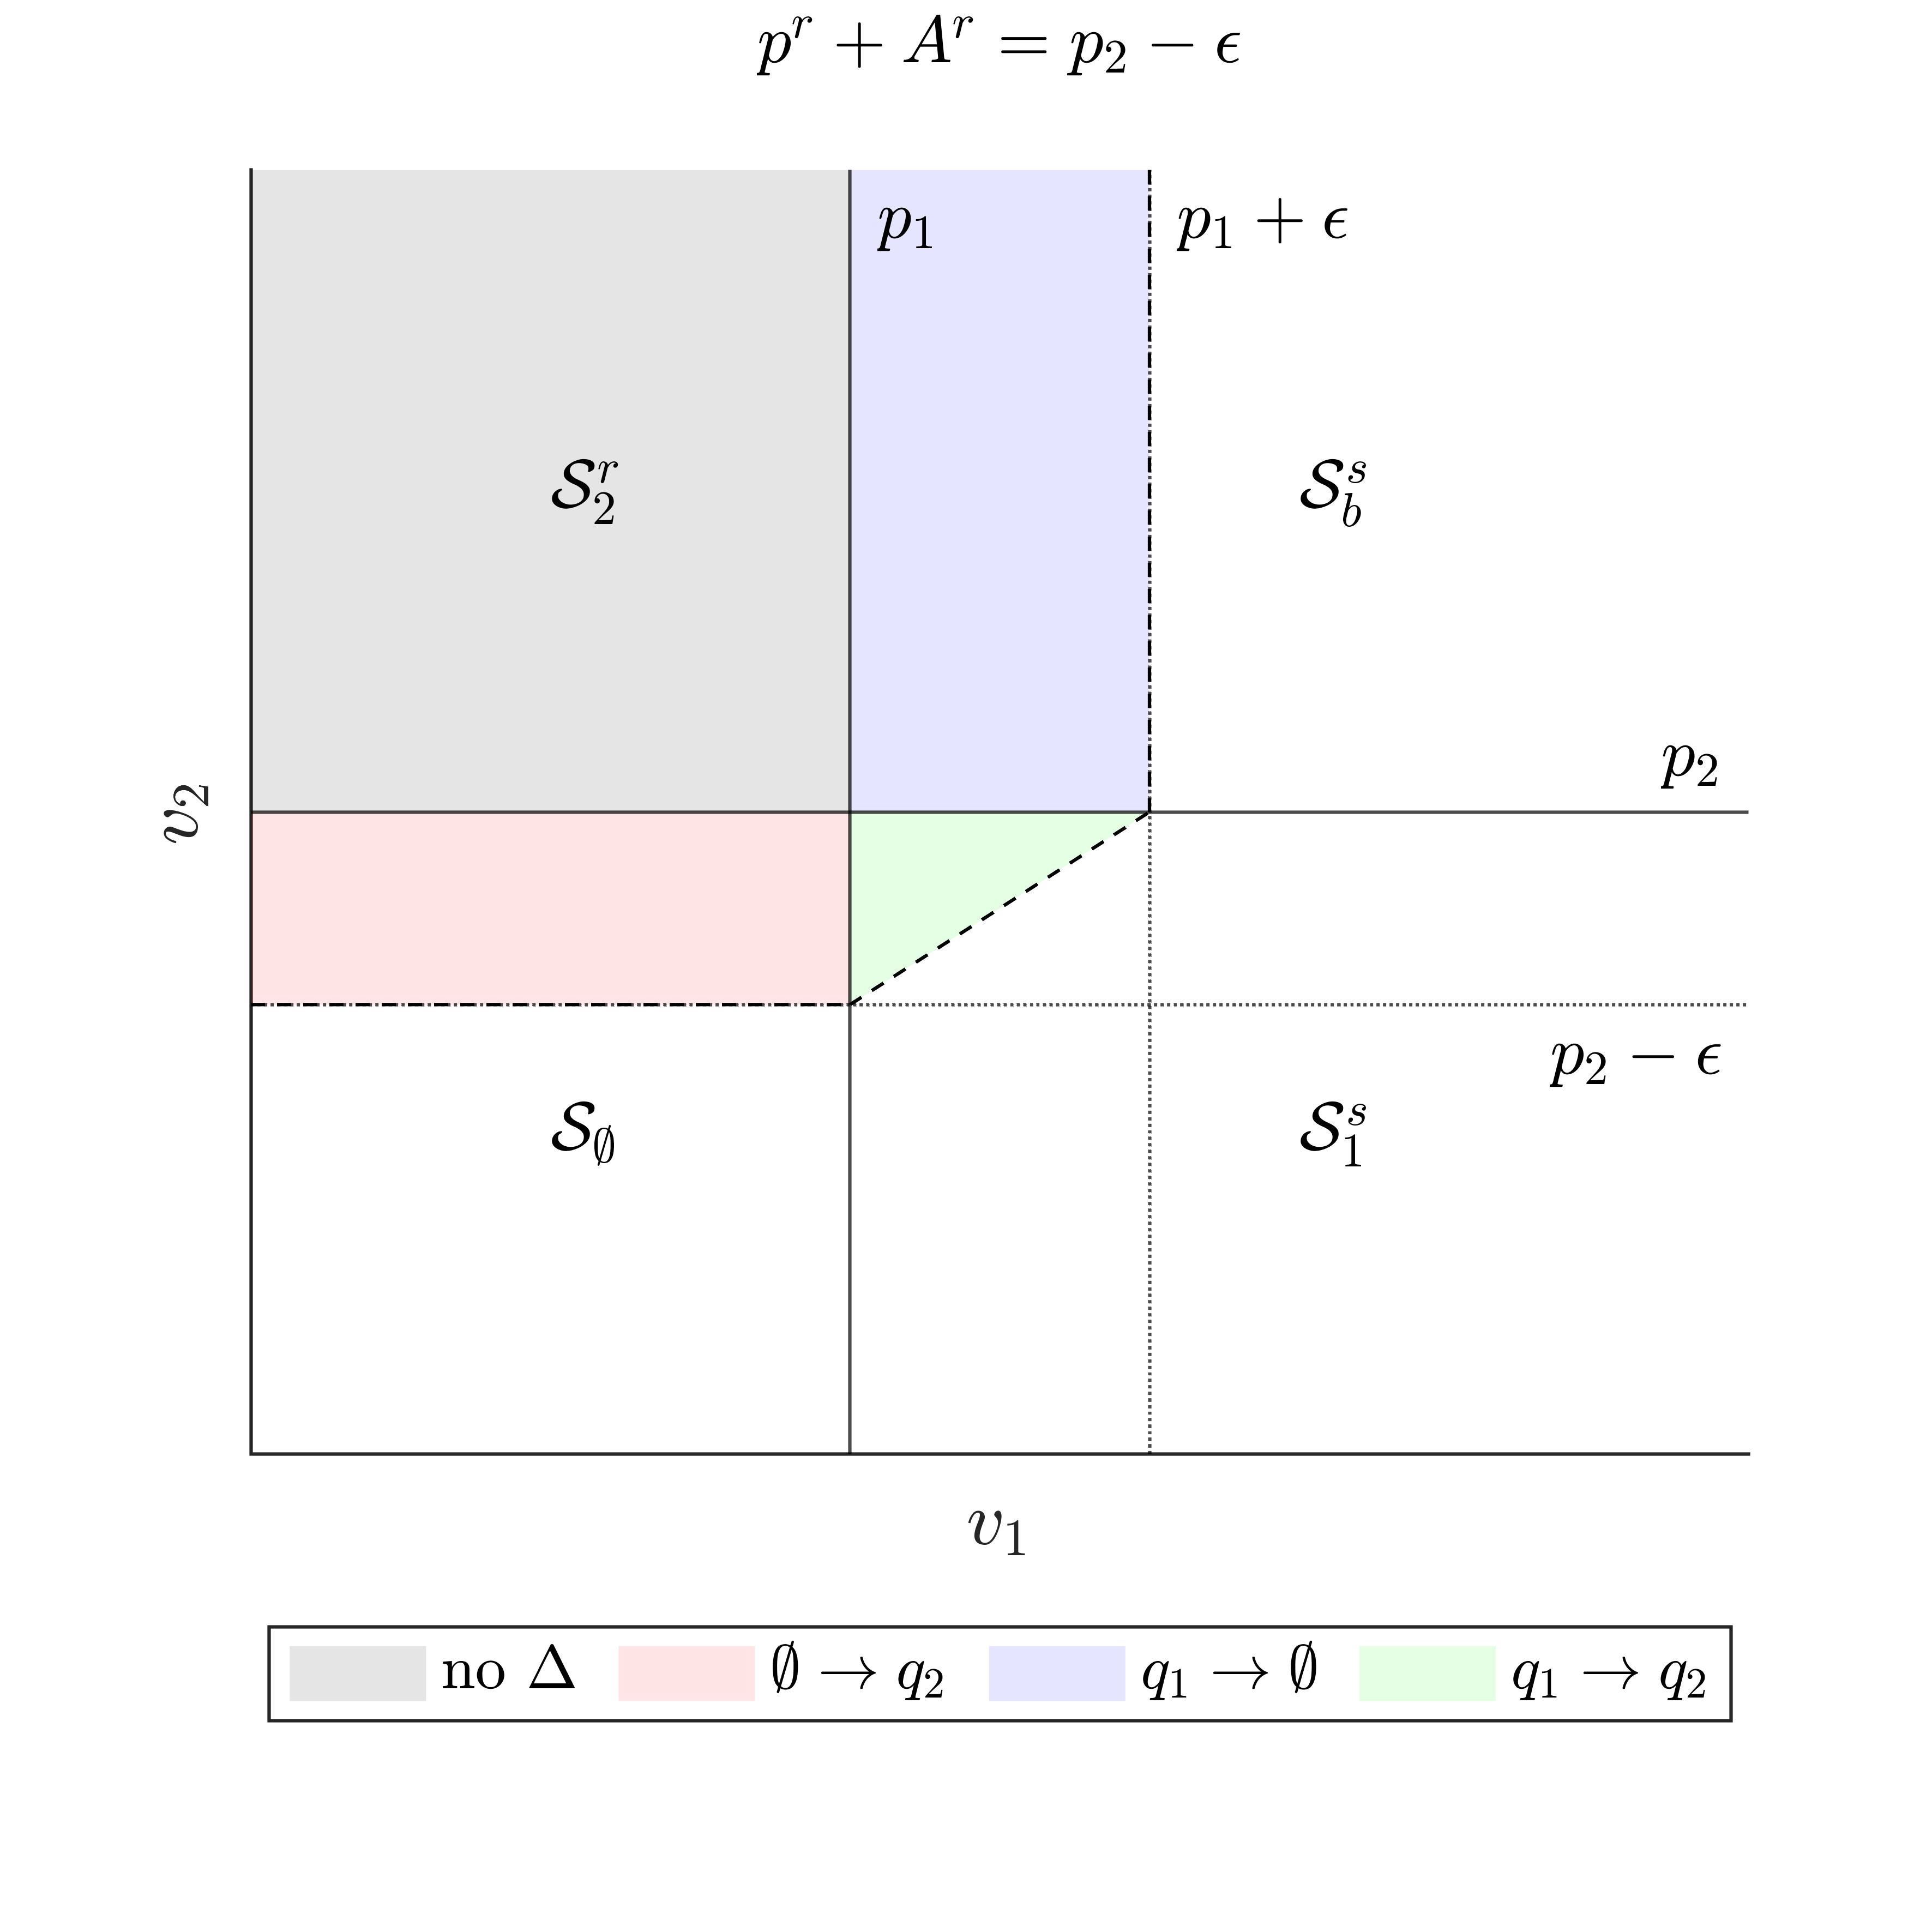
\includegraphics[width=1\linewidth]{figure/spot_demand_multi_sb_ppt.png}
    \caption{Downward price deviation of FP with entry.}
    \label{fig:spot_demand_multi_sb_ppt}
\end{figure}
    
\end{frame}


%%%%%%%%%%%%%%%%%%%%%%%%%%%%%%%%%%%%%%%%%%%%%%%%%%%%%%%%%%%%%%%%%%%%%%%%%%%%%%%%%%%%%%%%%%%%%%%%%%%%%%%%%%%%%%%%%%%%%%%%%%%%%%%%%%%%%%%%%%%%%%%%%%%%%%


\begin{frame}{Private Firms only offer dynamic contracts in equilibrium}\label{PrivateFirms2}


\begin{proposition}
 With private firms, there is no equilibrium with consumers having a strict preference for the fixed-price contract. 
\end{proposition}

\begin{figure}
    \centering
    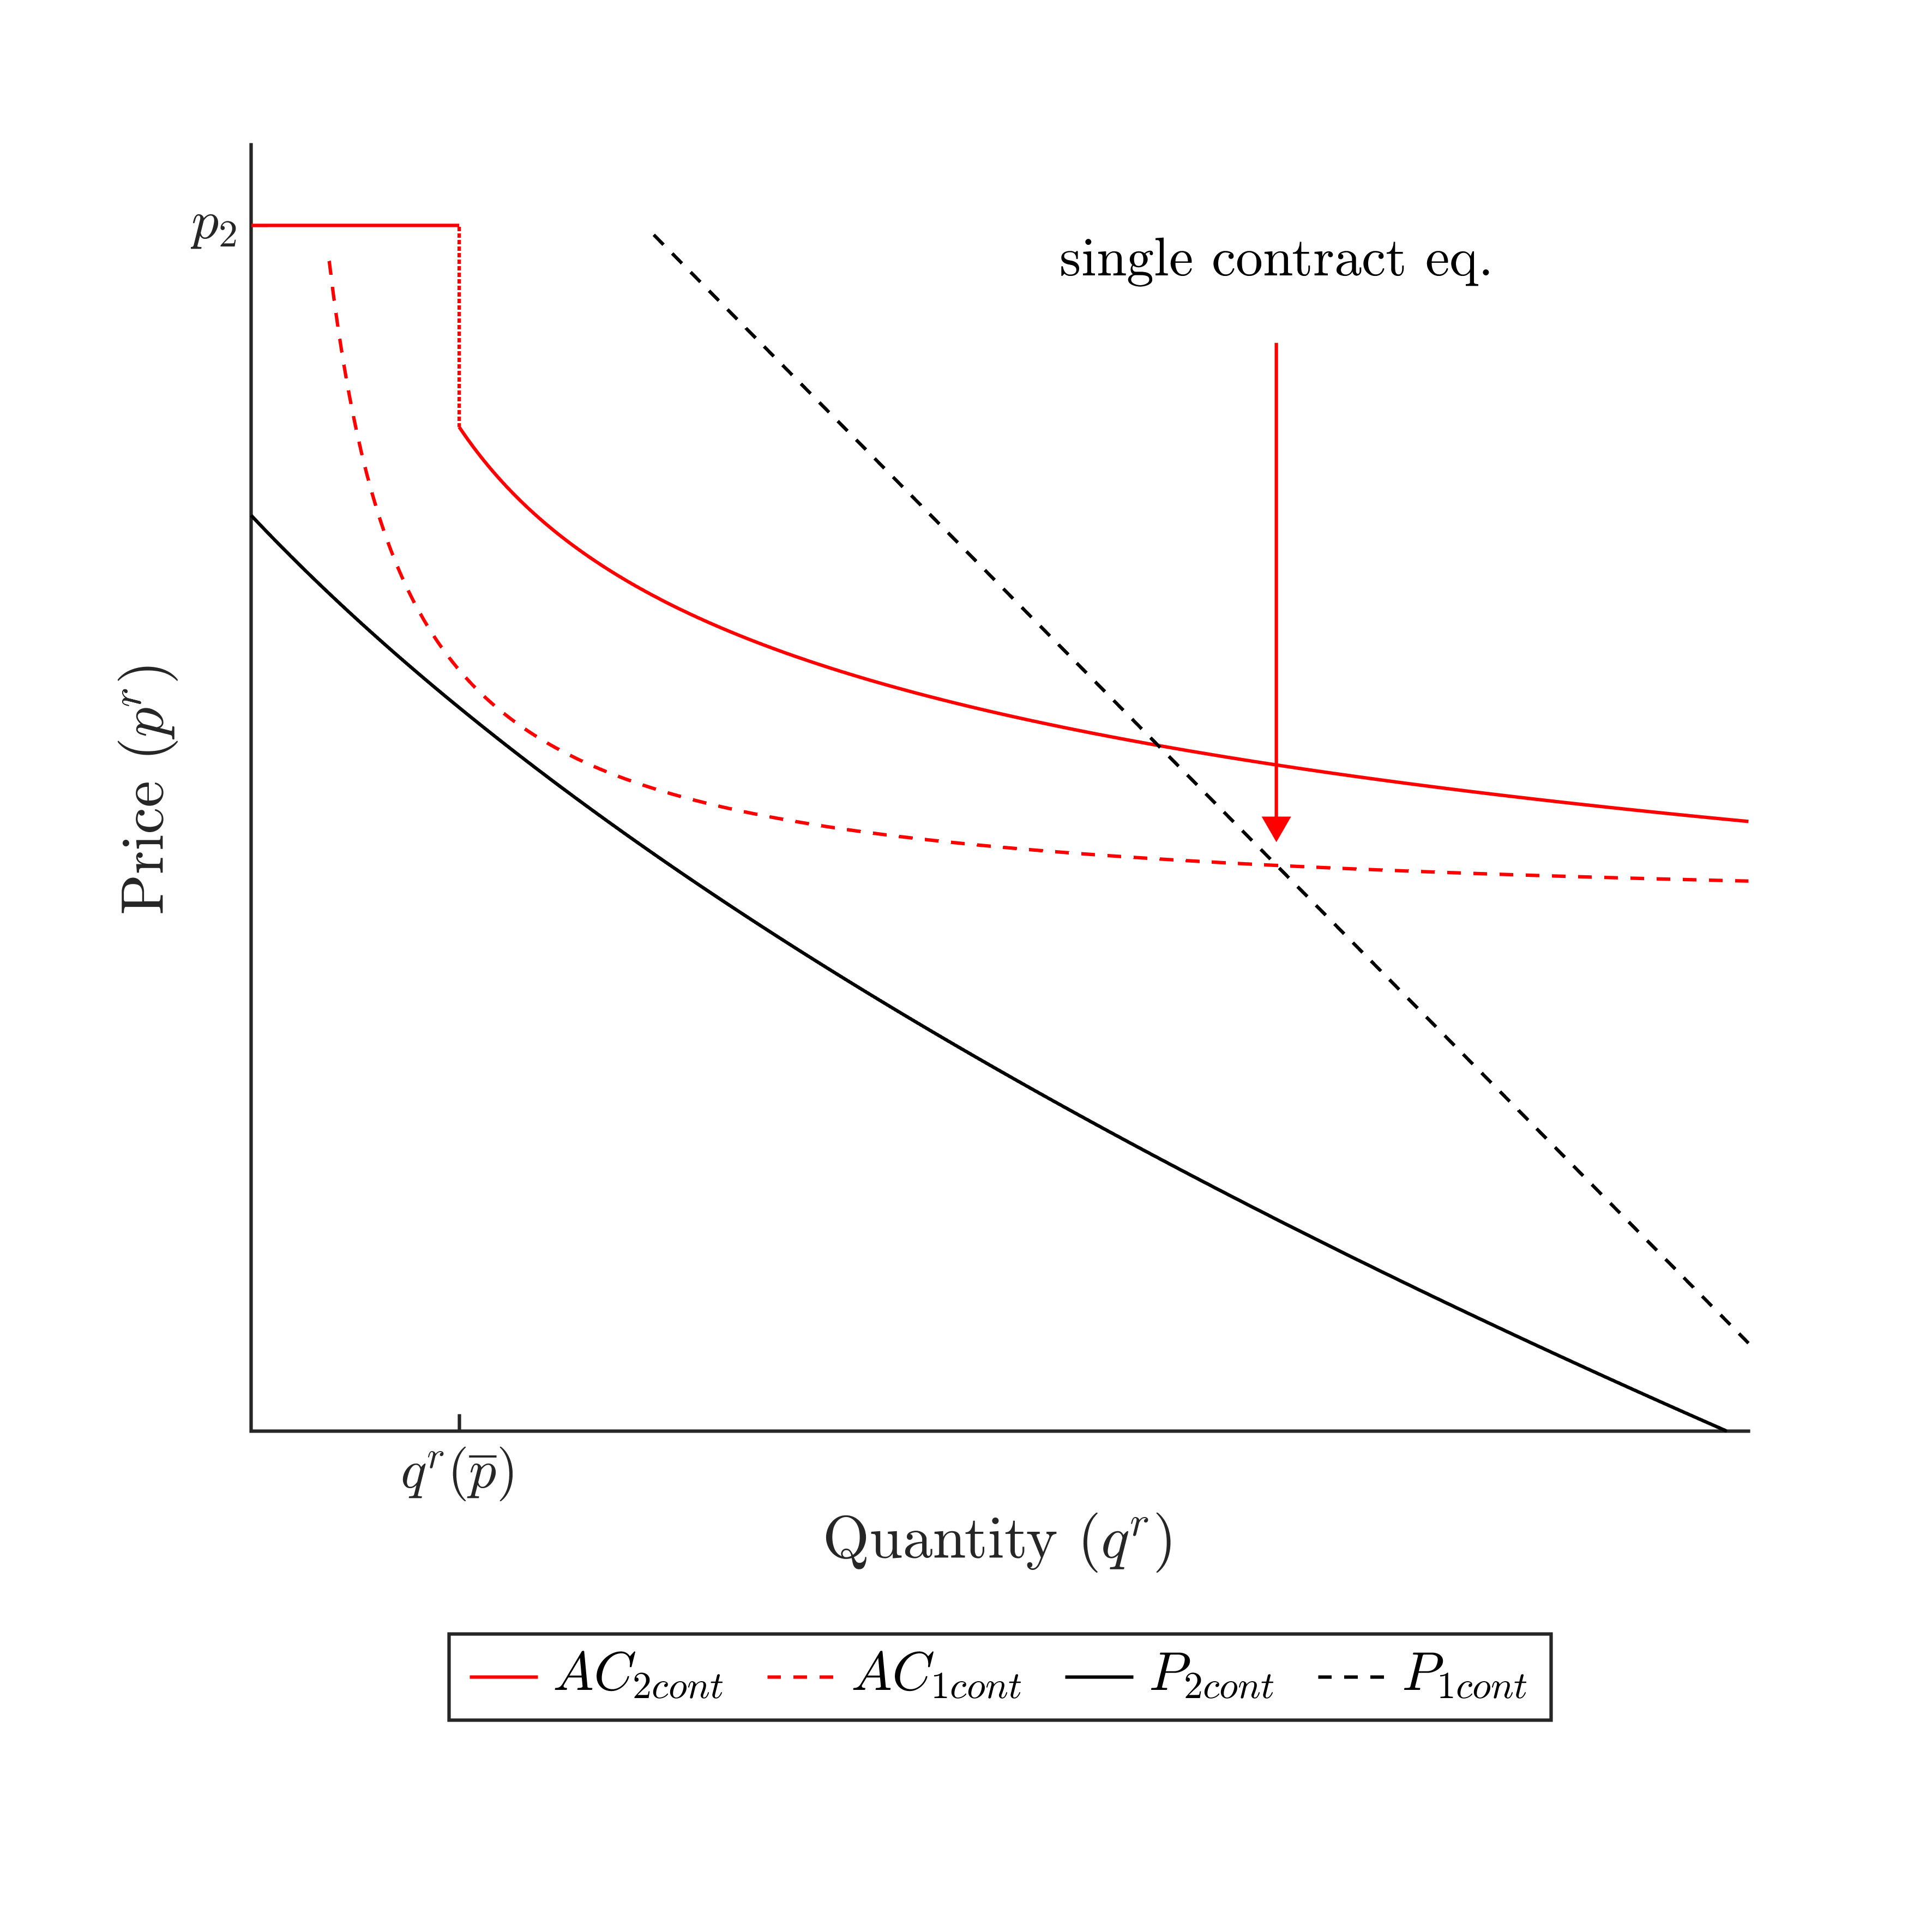
\includegraphics[width=0.8\linewidth]{figure/Exemple_Private_u_ddeAC_ppt.png}
\end{figure}
    
\end{frame}
% 


\begin{frame}{Ramsey Prices with Consumers Choice}\label{RamseyOutside}

Assume general objective function $CS^r + (1+\lambda) \pi^r$ and linear pricing $p^r$.

\vfill

Condition for equilibrium: $ W(\Omega_1) > \lambda q^r(p_2)$: 


\vfill

\begin{proposition}
 
With $\delta q$, the quantity derivatives, the linear price of the FP contract with the public firm solves the following modified Ramsey prices:
 

\begin{equation*}
      p^r \quad = \quad \;\underbrace{ \frac{\lambda}{1+\lambda} \frac{q^r}{\delta^p(q^r)}}_{\text{ramsey}} \; + \; \underbrace{p^w_1\frac{\delta q_1}{\delta^p(q^r)}+p^w_2\frac{\delta q_2}{\delta^p(q^r)}}_{\text{multi. types}} \; -  \;   \underbrace{\bigg. \Omega \bigg.}_{\text{foregone surplus}}  
\end{equation*}

\end{proposition}

\vfill

\begin{itemize}
    \item The model can easily be extended: $i$) two-part tariff, $ii$) Ramsey firm with endogenous $\lambda$, $iii$) and levy mechanism to pay for the public firm budget.
\end{itemize}


\end{frame}

%%%%%%%%%%%%%%%%%%%%%%%%%%%%%%%%%%%%%%%%%%%%%%%%%%%%%%%%%%%%%%%%%%%%%%%%%%%%%%%%%%%%%%%%%%%%%%%%%%%%%%%%%%%%%%%%%%%%%%%%%%%%%%%%%%%%%%%%%%%%%%%%%%%%%%

\begin{frame}{Incentive for fixed-price contract}

\begin{figure}
    \centering
    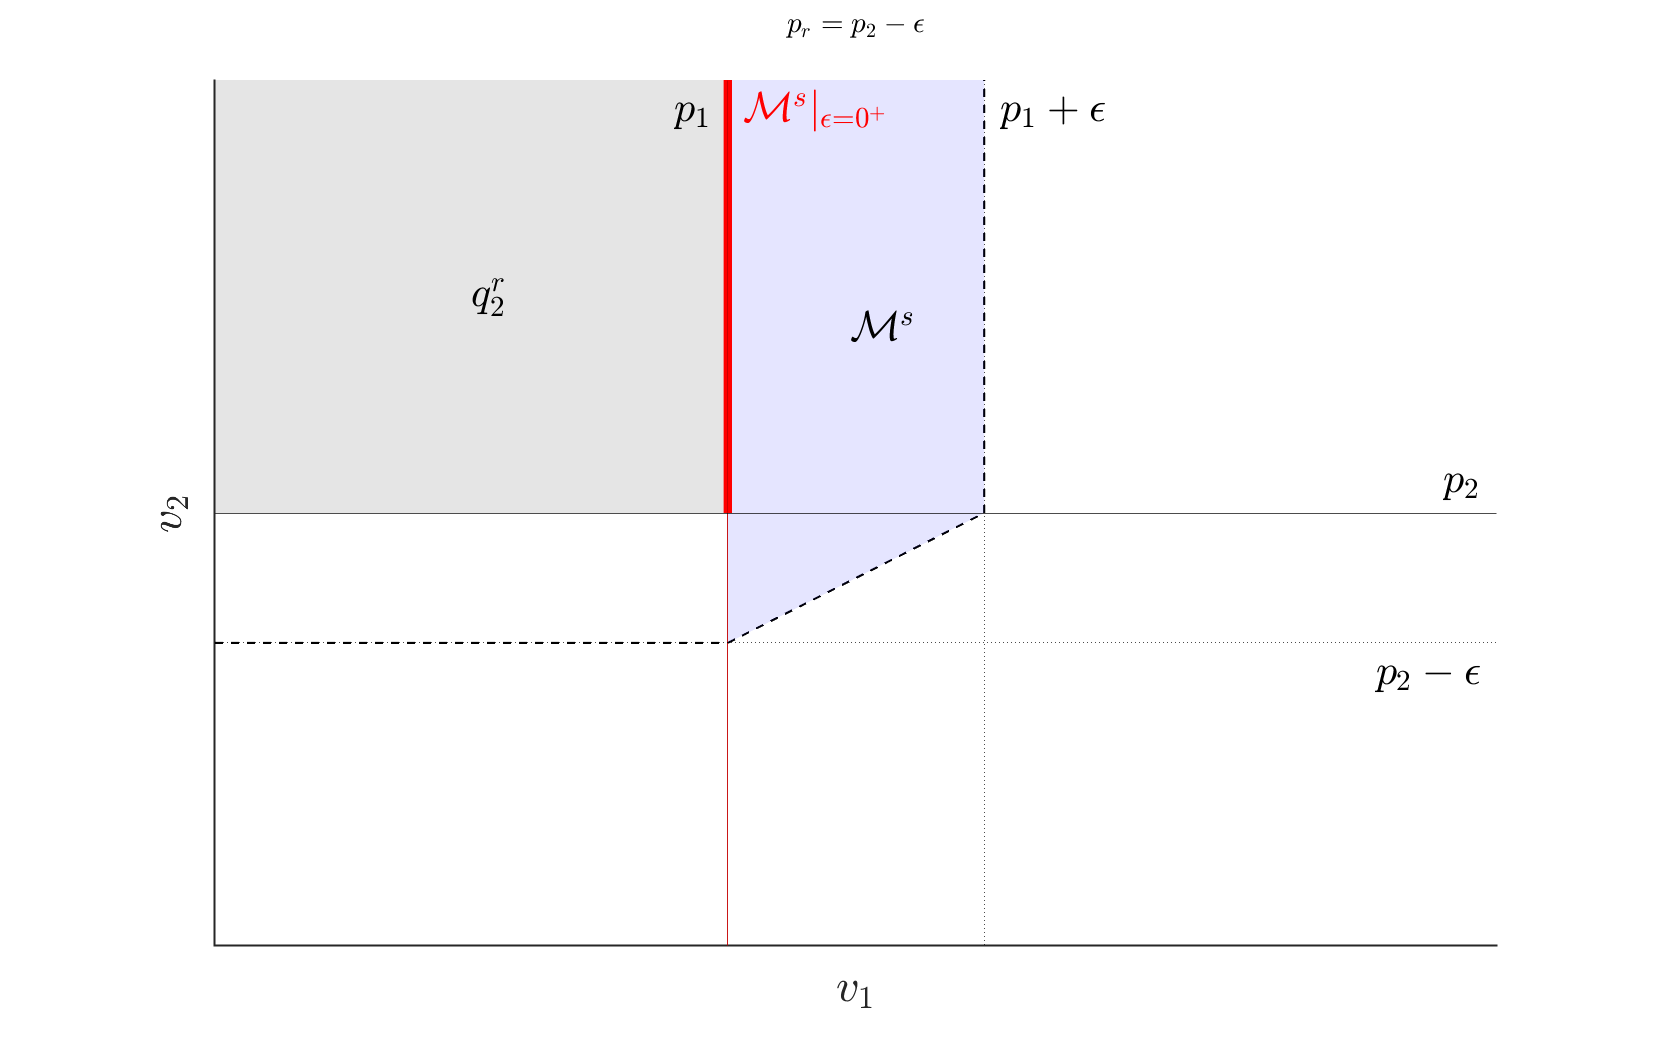
\includegraphics[width=1\linewidth]{figure/spot_demand_multi_sb_ppt_equil.png}
    \caption{Tradeoff for profitability of the public fixed-price contract.}
    \label{fig:spot_demand_multi_sb_ppt_equil}
\end{figure}
    
\end{frame}
%%%%%%%%%%%%%%%%%%%%%%%%%%%%%%%%%%%%%%%%%%%%%%%%%%%%%%%%%%%%%%%%%%%%%%%%%%%%%%%%%%%%%%%%%%%%%%%%%%%%%%%%%%%%%%%%%%%%%%%%%%%%%%%%%%%%%%%%%%%%%%%%%%%%%%

\begin{frame}{Implications of contract switchers}\label{IntuiRamsey}

\begin{figure}
    \centering
    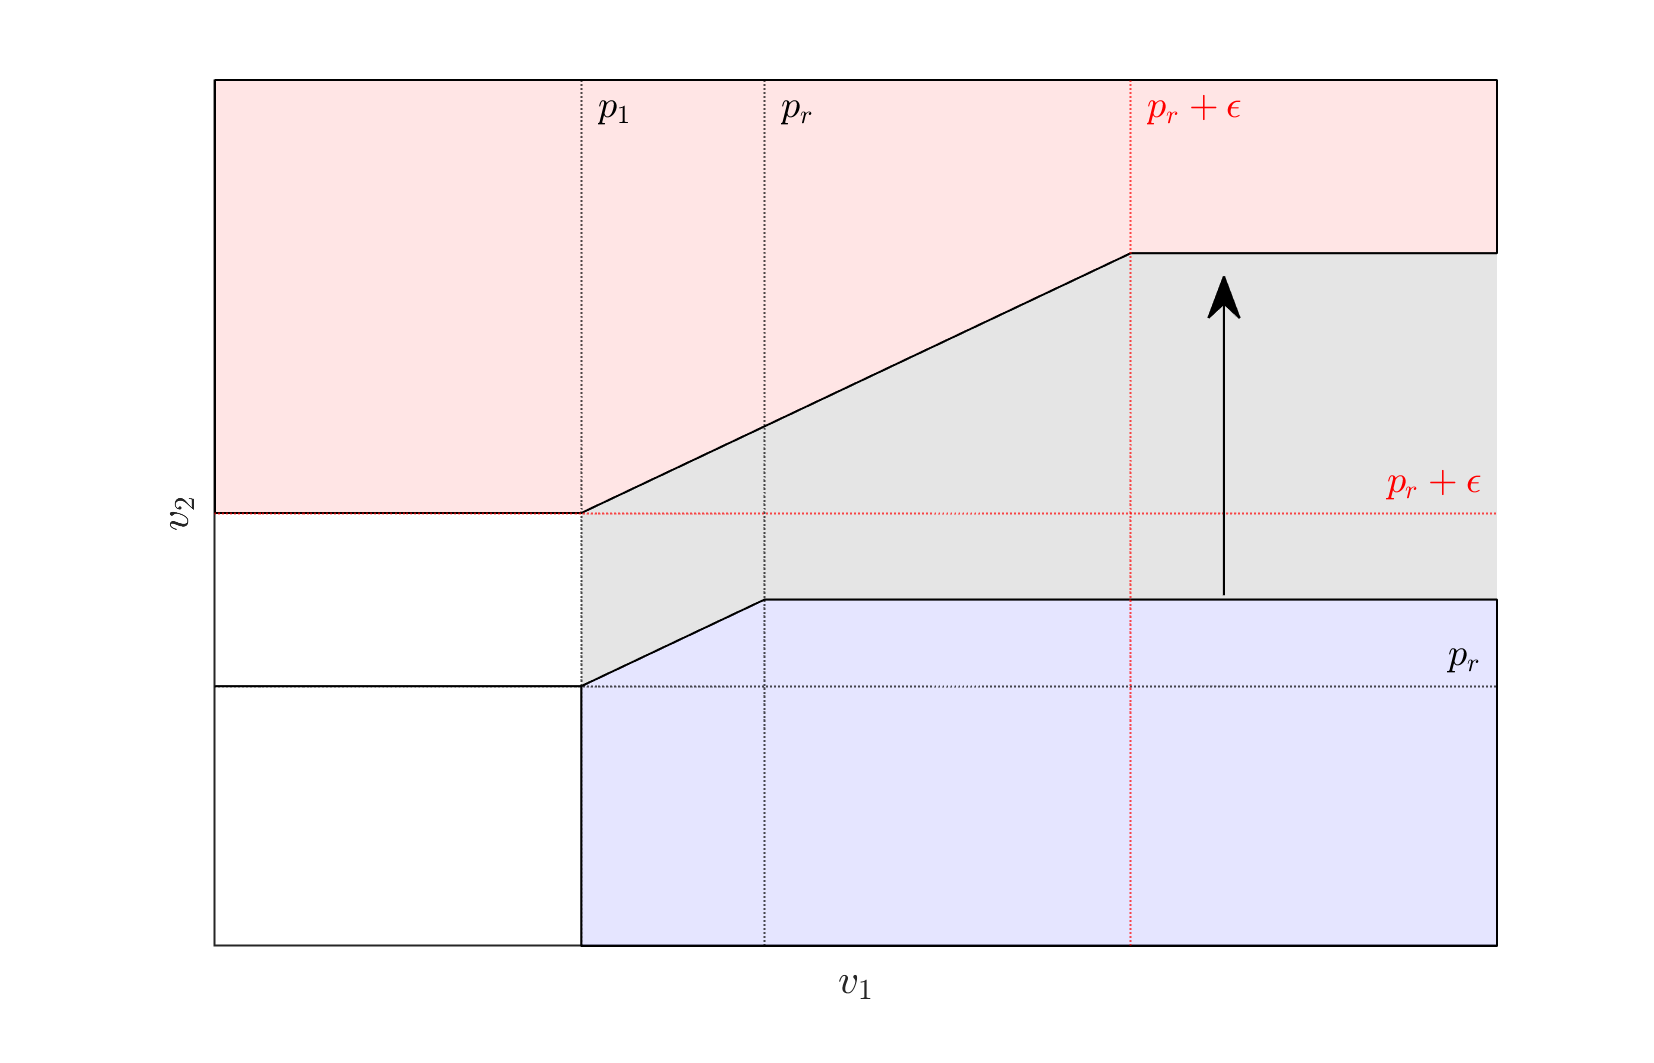
\includegraphics[width=0.95\linewidth]{figure/example_compstatpr_ppt.png}
    \caption{A marginal increases of the regulated fixed-price induces consumers to choose the private contract. $\Omega$ captures this welfare loss}
    
\end{figure}
    
\end{frame}

%%%%%%%%%%%%%%%%%%%%%%%%%%%%%%%%%%%%%%%%%%%%%%%%%%%%%%%%%%%%%%%%%%%%%%%%%%%%%%%%%%%%%%%%%%%%%%%%%%%%%%%%%%%%%%%%%%%%%%%%%%%%%%%%%%%%%%%%%%%%%%%%%%%%%%

\section{Welfare implication}

%%%%%%%%%%%%%%%%%%%%%%%%%%%%%%%%%%%%%%%%%%%%%%%%%%%%%%%%%%%%%%%%%%%%%%%%%%%%%%%%%%%%%%%%%%%%%%%%%%%%%%%%%%%%%%%%%%%%%%%%%%%%%%%%%%%%%%%%%%%%%%%%%%%%%%

\begin{frame}{Roadmap}
  \tableofcontents [sectionstyle=show/shaded,subsectionstyle=show/shaded]
\end{frame}

%%%%%%%%%%%%%%%%%%%%%%%%%%%%%%%%%%%%%%%%%%%%%%%%%%%%%%%%%%%%%%%%%%%%%%%%%%%%%%%%%%%%%%%%%%%%%%%%%%%%%%%%%%%%%%%%%%%%%%%%%%%%%%%%%%%%%%%%%%%%%%%%%%%%%%

\begin{frame}{Welfare comparison}


\begin{itemize}
   
    \item Only private firms: \boldrblue{ First-Best}. \vfill

    \item Public Firm + Private Firms + Consumer Choices \boldrblue{?} \vfill

    \item We compare the welfare with \boldrblue{a Single Contract} environment. \vfill

    \begin{itemize}
        \item We show that the \boldrblue{welfare can be ambiguous}. \vfill
        \item Due to having \boldrblue{a lower fixed-price} compared to the single contract case.
    \end{itemize}
    
\end{itemize}
    
\end{frame}

%%%%%%%%%%%%%%%%%%%%%%%%%%%%%%%%%%%%%%%%%%%%%%%%%%%%%%%%%%%%%%%%%%%%%%%%%%%%%%%%%%%%%%%%%%%%%%%%%%%%%%%%%%%%%%%%%%%%%%%%%%%%%%%%%%%%%%%%%%%%%%%%%%%%%%

% \begin{frame}{The intuitions}\label{WelfareComp}

% \begin{enumerate}
%     \item Allowing self-selection from consumers implies that a specific set of consumers leaves the public firm. \vfill
%     \item High-$v_1$ consumers are particularly valuable in terms of surplus. \vfill
%     \item It puts downward pressure on the firm to avoid surplus loss: $p^r^{choice} < \textcolor{red}{p^r^{single}}$ \vfill
%     \item But it implies more over-consumption from low-$v_2$ consumers. 
%     \vfill 
%      \item There exists some set of parameters such that \boldrblue{Losses from consumers over-consuming} out-weight the \boldrblue{Gains from consumers switching to the dynamic contract}.
% \end{enumerate}
    
% \end{frame}

%%%%%%%%%%%%%%%%%%%%%%%%%%%%%%%%%%%%%%%%%%%%%%%%%%%%%%%%%%%%%%%%%%%%%%%%%%%%%%%%%%%%%%%%%%%%%%%%%%%%%%%%%%%%%%%%%%%%%%%%%%%%%%%%%%%%%%%%%%%%%%%%%%%%%%



\begin{frame}{Application - Equilibrium and Welfare}

\begin{figure}
    \centering
    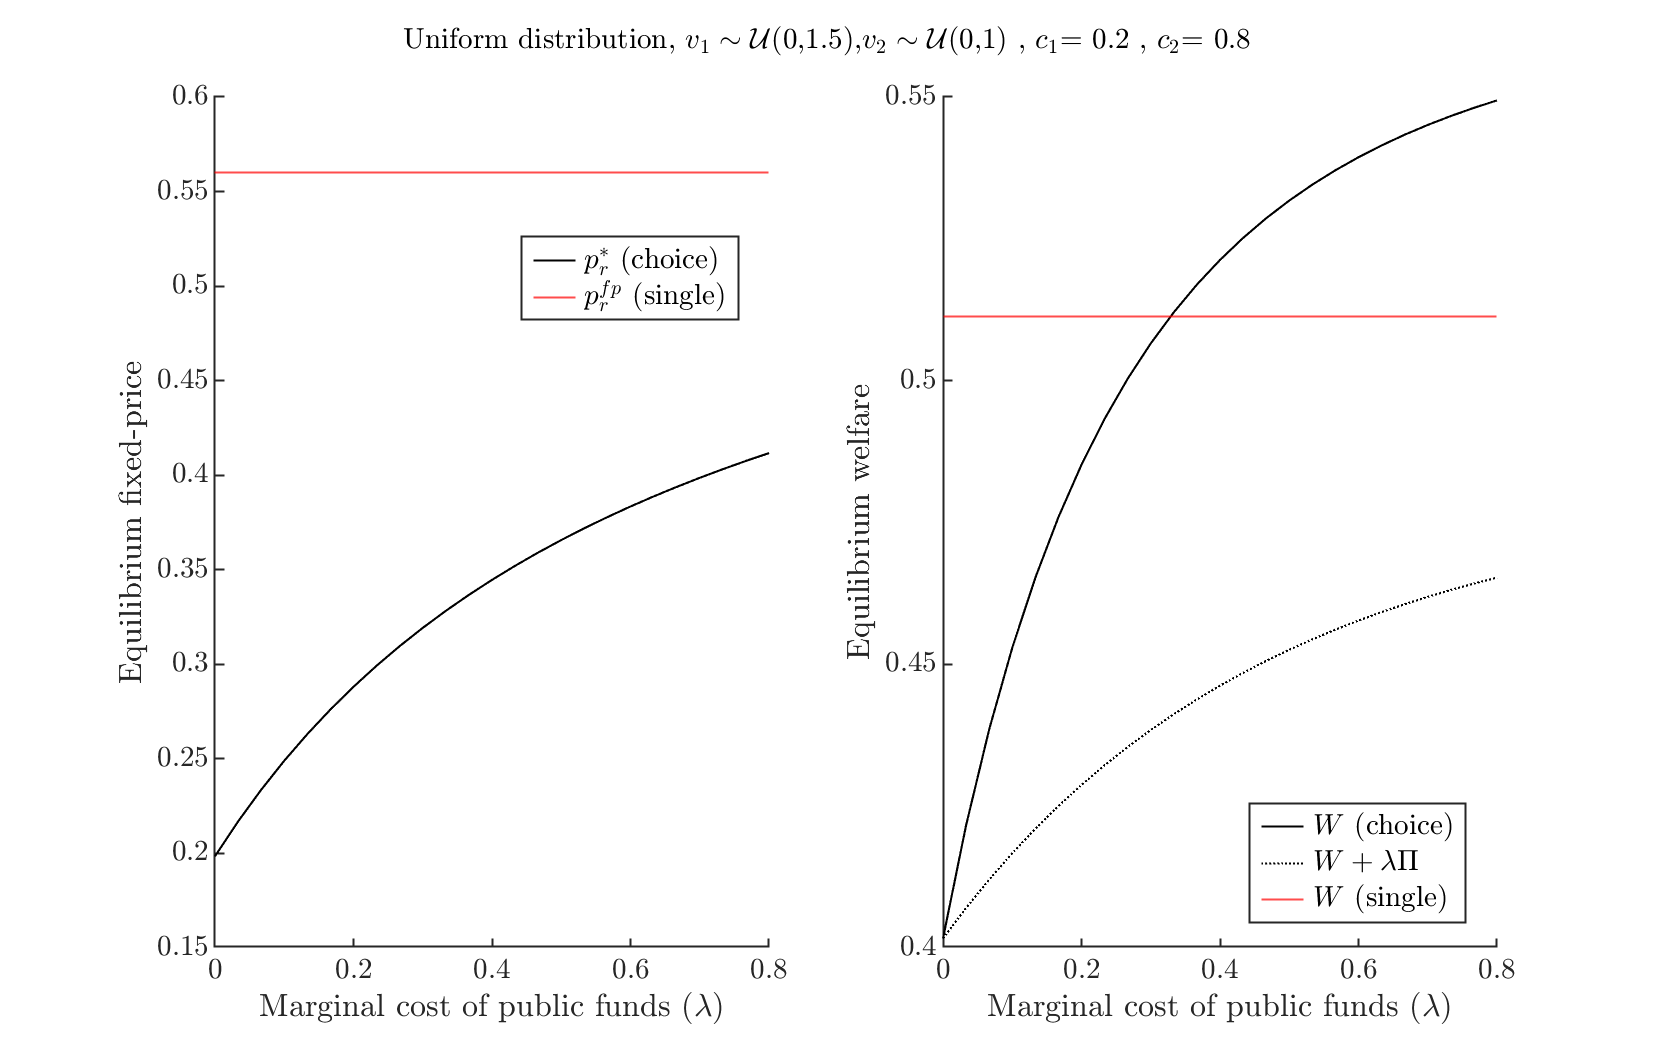
\includegraphics[width=1\linewidth]{figure/example_equ0_u.png}
\end{figure}
    
\end{frame}

%%%%%%%%%%%%%%%%%%%%%%%%%%%%%%%%%%%%%%%%%%%%%%%%%%%%%%%%%%%%%%%%%%%%%%%%%%%%%%%%%%%%%%%%%%%%%%%%%%%%%%%%%%%%%%%%%%%%%%%%%%%%%%%%%%%%%%%%%%%%%%%%%%%%%%

\begin{frame}{Application - Equilibrium}

\begin{figure}
    \centering
    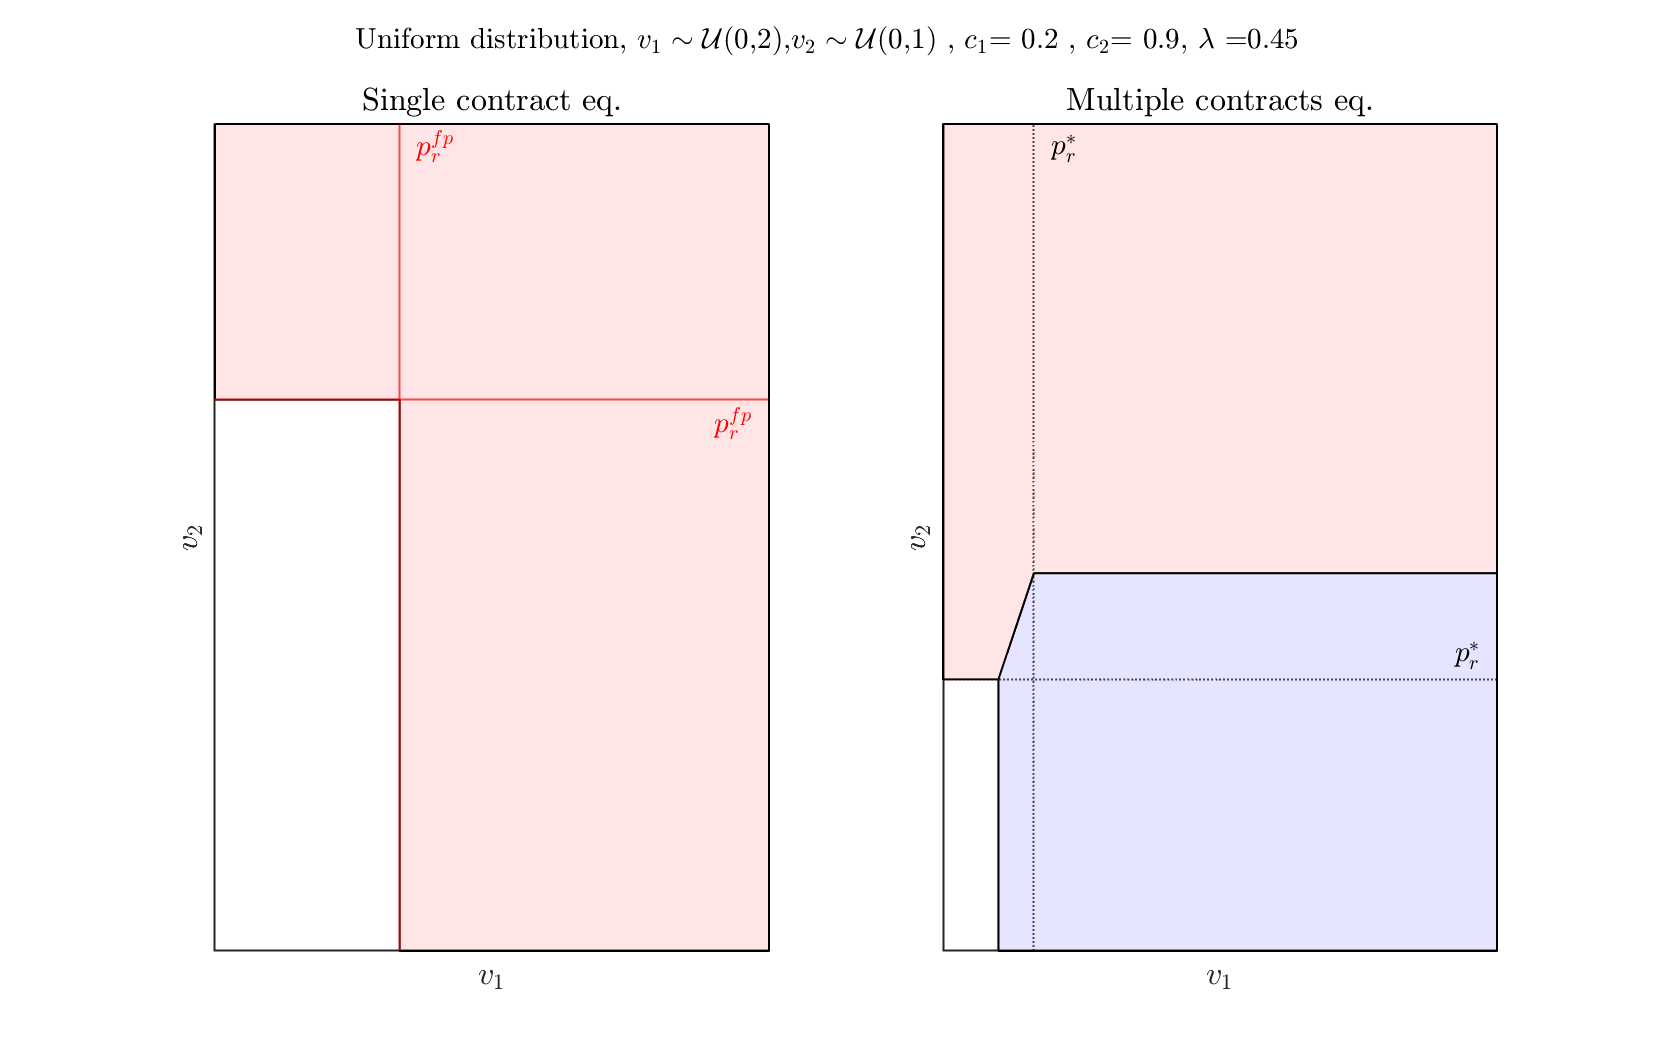
\includegraphics[width=0.95\linewidth]{figure/example_equ1_u.png}
\end{figure}
    
\end{frame}

%%%%%%%%%%%%%%%%%%%%%%%%%%%%%%%%%%%%%%%%%%%%%%%%%%%%%%%%%%%%%%%%%%%%%%%%%%%%%%%%%%%%%%%%%%%%%%%%%%%%%%%%%%%%%%%%%%%%%%%%%%%%%%%%%%%%%%%%%%%%%%%%%%%%%%

\begin{frame}{Application - Adverse selection at play}

\begin{figure}
    \centering
    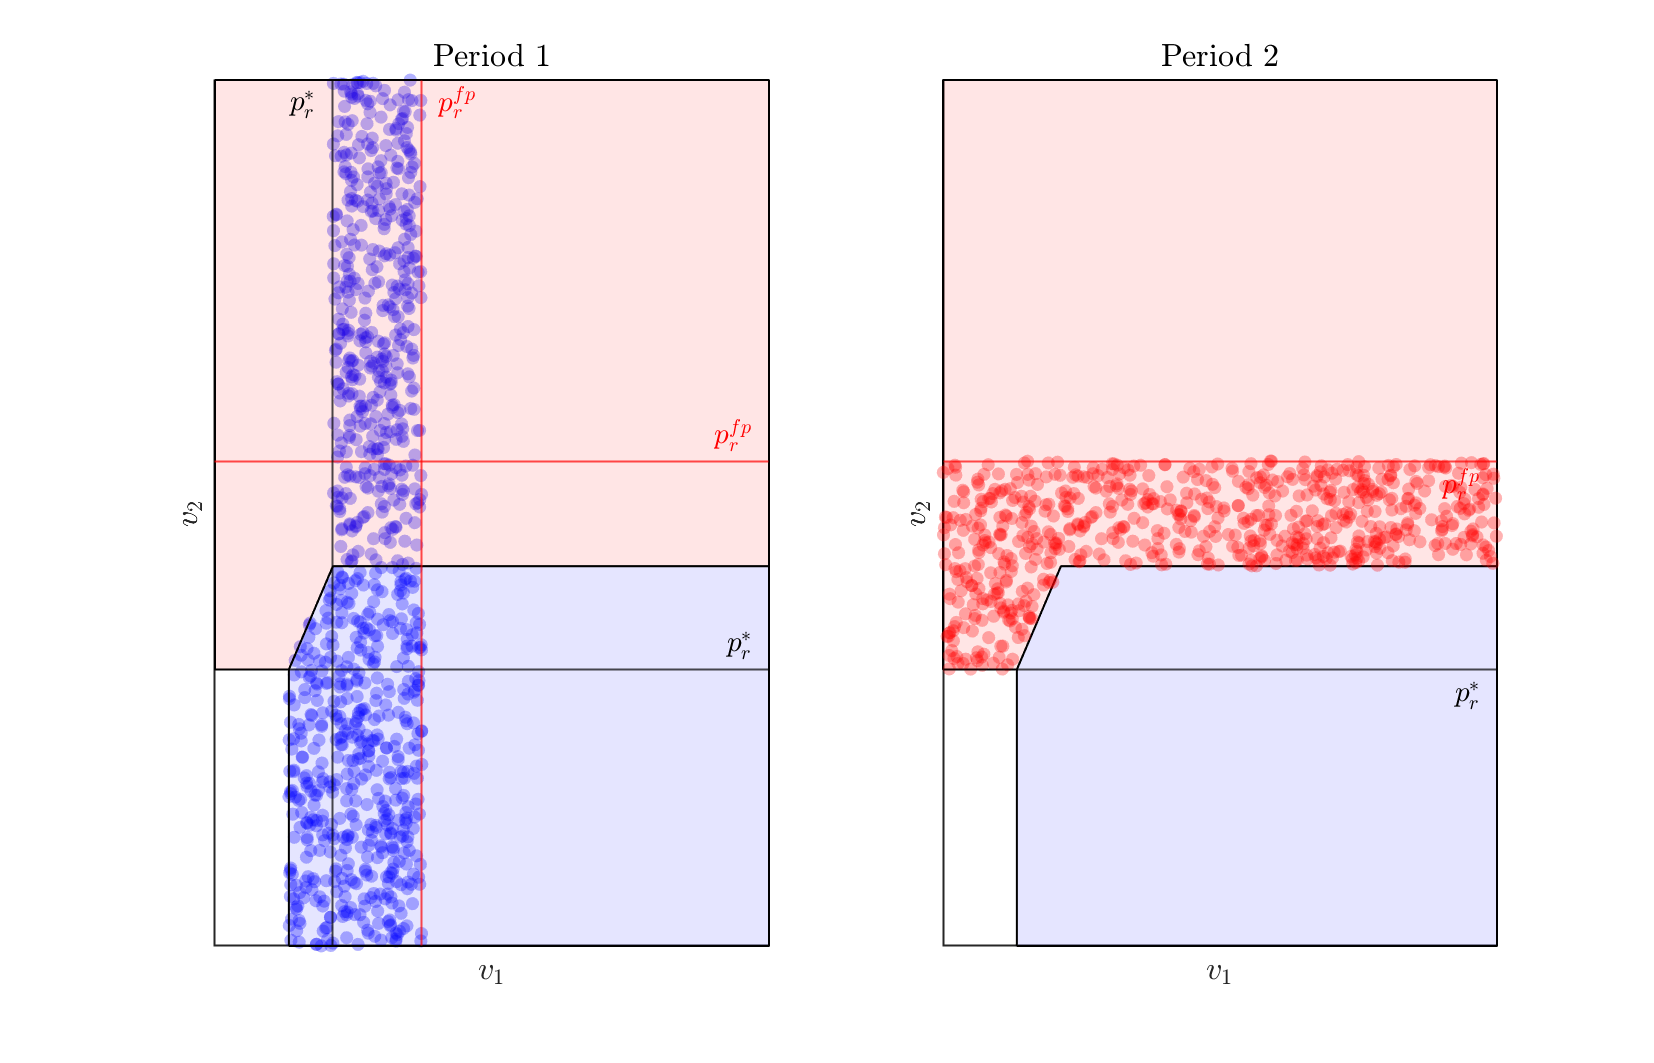
\includegraphics[width=0.95\linewidth]{figure/example_equ2_u.png}
\end{figure}
    
\end{frame}


%%%%%%%%%%%%%%%%%%%%%%%%%%%%%%%%%%%%%%%%%%%%%%%%%%%%%%%%%%%%%%%%%%%%%%%%%%%%%%%%%%%%%%%%%%%%%%%%%%%%%%%%%%%%%%%%%%%%%%%%%%%%%%%%%%%%%%%%%%%%%%%%%%%%%%

\section{Conclusion}

\begin{frame}{Literature}

\begin{itemize}
    \item No theory of self-selection in power retail market.
    \begin{itemize}
        \item Seminal paper: \cite{Borenstein2005b}, Technological cost \cite{Leautier2014},  Interactions with renewable technologies \cite{Ambec2021}, Risk aversion \cite{Boom2021}.
        \item \boldrblue{limits}: exogenous share - single period - homogeneous consumers. \vfill
    \end{itemize}

    \item Scarce papers on the supply side of retail contracts.
    \begin{itemize}
    \item  Seminal papers \cite{joskow2006retail} and \cite{Borenstein2003}.
    \item \boldrblue{limits}: homogeneous consumers - simplified market structure.\vfill
    \end{itemize}

    \item Two streams of theory
    \begin{itemize}
        \item \boldrblue{Adverse Selection}. price equilibrium \cite{1970Akerlof}, price theory \cite{Einav2012}, multidimensional setting \cite{Veiga2016}, competition \cite{Azevedo2017}.
        \item \boldrblue{Public option with incomplete information} regulated firm \cite{laffont1993theory}, electricity markets \cite{Martimort2020a} mechanism design \cite{Kang2023a}.
    \end{itemize}
    
\end{itemize}
    
\end{frame}


\begin{frame}{Conclusion}

\begin{itemize}
    \item The paper provides a novel framework describing the self-selection of electricity contracts by heterogeneous consumers.\vfill
    \item We characterize the contracts' price equilibrium in different retail market structures.\vfill
    \item We show that the coexistence of a public option with a private sector and self-selection from consumers can lead to low welfare due to adverse selection.\vfill
    \item The mode provides some foundations for multiple extensions, including public policy in incomplete information and long-term decisions in clean technology, both from consumers and producers.
\end{itemize}
    
\end{frame}



%%%%%%%%%%%%%%%%%%%%%%%%%%%%%%%%%%%%%%%%%%%%%%%%%%%%%%%%%%%%%%%%%%%%%%%%%%%%%%%%%%%%%%%%%%%%%%%%%%%%%%%%%%%%%%%%%%%%%%%%%%%%%%%%%%%%%%%%%%%%%%%%%%%%%%


\begin{frame}{}
  \centering {\Huge
  \emph{Thank you !}}
  
  \vspace{1cm}

  http://leopoldmonjoie.com/
\end{frame}


\newcounter{totalbeforeappendix}
\setcounter{totalbeforeappendix}{\value{framenumber}}
\addtocounter{totalbeforeappendix}{2} 
\addtocounter{framenumber}{-26}


\begin{frame}{Literature: Demand for contracts}\label{Lit_Conso}

\begin{itemize}
    \item \textbf{No theoretical foundation of self-selection in the power retail market}.

    \vfill
    
    \item Variation of a share of dynamic consumers.
    \begin{itemize}
        \item Seminal paper: \cite{Borenstein2005b}, Technological cost \cite{Leautier2014},  Interactions with renewable technologies \cite{Ambec2021}, Risk aversion \cite{Boom2021}.
        \item \boldrblue{limits}: exogenous share - single period - homogeneous consumers. 
    \end{itemize}

 \vfill

    \item \boldrblue{Empirical evidence} of self-selection with heterogeneous consumers
    \begin{itemize}
        \item Adverse selection \cite{Ito2023} Risk aversion \cite{Qiu2018} Behavioral bias \cite{Hortacsu2017,Fowlie2021}
        \item \boldrblue{limits}: focus on behavioral biais.
    \end{itemize}


\vfill
    \item Empirical evidence of RTP contracts.
    
    \begin{itemize}
        \item Effect of contract prices on consumption \cite{Fabra2021,Han2023,Enrich2024,Fu2024}, Redistributive effect \cite{Leslie2021, Levinson2022a, Cahana2023}
    \end{itemize}


     
    
\end{itemize}

\vfill

\hyperlink{FirstCont}{\beamergotobutton{Back}}

\end{frame}

%%%%%%%%%%%%%%%%%%%%%%%%%%%%%%%%%%%%%%%%%%%%%%%%%%%%%%%%%%%%%%%%%%%%%%%%%%%%%%%%%%%%%%%%%%%%%%%%%%%%%%%%%%%%%%%%%%%%%%%%%%%%%%%%%%%%%%%%%%%%%%%%%%%%%%

\begin{frame}{Literature: Retail competition}\label{Lit_Mkt1}
    
    
\begin{itemize}
    \item \textbf{Little attention on the competition in the retail market and contract equilibrium}.  
    
    \vfill

    \item Few empirical works on the benefit of retail competition \cite{Concettini2013}. Retailers acting as in Bertrand competition \cite{von2010electricity}
    
    \vfill

   \item Seminal papers \cite{joskow2006retail} and \cite{Borenstein2003}. \boldrblue{limits}: homogeneous consumers - simplified market structure.

\vfill

   \item  \boldrblue{Adverse selection} in retail electricity market
   
   \begin{itemize}
       \item Consumers deviation \cite{chao2013incentive}
       \item IC contracts and market equilibrium \cite{Astier2021}
   \end{itemize}

\vfill

    \item \boldrblue{Outside public option with incomplete information}
    \begin{itemize}
        \item In electricity markets with a regulated firm with redistributive preferences \cite{Martimort2020a} in a general setting \cite{Kang2023a}
    \end{itemize}


% \vfill

% \item Market power and price discrimination in retail electricity market \cite{byrne2022price}

\end{itemize}

\vfill



\hyperlink{SecondCont}{\beamergotobutton{Back}}

\end{frame}


%%%%%%%%%%%%%%%%%%%%%%%%%%%%%%%%%%%%%%%%%%%%%%%%%%%%%%%%%%%%%%%%%%%%%%%%%%%%%%%%%%%%%%%%%%%%%%%%%%%%%%%%%%%%%%%%%%%%%%%%%%%%%%%%%%%%%%%%%%%%%%%%%%%%%%

\begin{frame}{Literature: Other litterature }\label{Lit_Mkt2}
    
    
\begin{itemize}

   \item \textbf{Adverse Selection}
   \begin{itemize}
       \item Selection on the level and selection on the slope \cite{Einav2011,Einav2021}
       \item Empirical evidence for electricity contracts \cite{Ito2023}
   \end{itemize}


\vfill

   \item \textbf{Self-Selection}
    \begin{itemize}
        \item Roy Model \cite{Barro2013}
        \item Applied to Energy Efficiency \cite{Allcott2014}
    \end{itemize}

\vfill

   \item \textbf{Durable Goods}
   \begin{itemize}
       \item Household as production unit \cite{Becker1965}
       \item Applied to short-term/long-term decisions \cite{Feger2022} 
   \end{itemize}

\vfill

   \item \textbf{Competition for non-linear contracts}
   \begin{itemize}
       \item General setting \cite{Stole2007}
       \item Applied to insurance \cite{Rothschild1976,Dosis2022} 
   \end{itemize}
   
\vfill

   \item \textbf{Multidimensional Screening} \cite{Rochet1998}
   
\end{itemize}
\vfill

\hyperlink{SecondCont}{\beamergotobutton{Back}}

\end{frame}



\end{document}
